\part{初级句型——简单句}

\chapter{基本句型及补语}

\section{五种单句的基本句型}

\begin{longtable}[]{@{}llll@{}}
  1. & S+V & 主语 + 动词 & \\
  2. & S+V+O & 主语 + 动词 + 宾语 & S:主语 Subject \\
  3. & S+V+C & 主语 + 动词 + (主语)补语 & V:动词 Verb \\
  4. & S+V+O+O & 主语 + 动词 + (间接)宾语 + (直接)宾语 & O:宾语 Object \\
  5. & S+V+O+C & 主语 + 动词 + 宾语 + (宾语)补语 & C:补语 Complement
\end{longtable}

虽然从初中开始就教五种基本句型,可是其中有两种(句型 3 和 句型5)关
于\textbf{补语}的句型,许多人恐怕一直没有真正搞清楚是怎么回事。如果有五分之二的简单
句没有弄懂,接下来的复句可就没办法弄清楚了。所以补语是第一个需要加强的观念。

要了解补语,只需要研究那些解释为“是”的动词。基本句型分五种,是因为有五种特
性不同的动词而造成的。\textbf{在所有的英语动词中,只有解释为“是”的动词(系动词)
  是空的,完全没有意义,也只有这种动词必须接补语来补足句子的意思。}

先回到出发点来说。一个完整的句子,必须能够表达完整的意思。这需要以两个部分来
完成:主语和动词。\textbf{主语,是这个句子所叙述的对象。动词,构成叙述的主要内容。}例
如:

\begin{enumerate}
\item John Smith died in World War Two.

  约翰·史密斯死于第二次世界大战。
\item John Simth killed three enemy soldiers.

  约翰·史密斯杀了三名敌军士兵。
\end{enumerate}

在例 1 中,主语 John Smith是这个句子所叙述的对象。讲白一点就是:这个句子要告
诉你的是有关 John Smith 的事情。是什么事情呢?主要是:他“死了”(died)。动
词 died构成叙述的主要内容。至于说他死在第一次大战还是第二次大战,则是可有可无
的细节,以介词短语in World War Two 来表示,依附在动词上做修饰语使用。换句话说,
例 1如果只说 John Smith died,也可以构成意思完整、正确的句子。

像 die这种动作,可以独立发生,不牵涉到别的人或物,这种动词就叫“\textbf{不及物}”动词。
可是像例2 中 kill这种动作,就必须发生在另一个对象的身上。要做出“\textbf{杀}”的动作,
得有个东西“\textbf{被杀}”才行,“杀”这种动词就叫“及物”动词,它后面通常必须跟着一
个\textbf{宾语来“接受”这个动作}。例2 中,killed 就是及物动词,而 three enemy
soldiers 就是宾语。

接下来要进入重点所在了。在例 2 中,killed虽然需要宾语,可是句子最主要的内容还
是在主语、动词这两个部分。主语部分告诉我们这个句子要叙述有关John Smith 的事情;
动词部分叙述他做了个“杀”的动作。如果只说 John Smith killed,那么这个句子还
没有表达出完整的意思,是不好的句子。可是,它并非完全没有意义,至少我们可以看
出来,有一个叫John Smith 的人杀了个不晓得是什么的东西。

反之,如果句子\textbf{缺了补语,就会变得完全没有意义},因为叙述的部分完全缺乏。请注
意:在所有的英语动词中,只有解释为“是”的动词是空的,完全没有意义。一般的动
词,不论及物或不及物,都要担任叙述全句最主要内容的工作。只有解释为“是”的动
词,没有叙述能力,只能扮演引导叙述部分的角色。例如:

\begin{enumerate}
  \setcounter{enumi}{2}
\item John Smith was a soldier.

  约翰·史密斯是军人。
\item John Smith was courageous.

  约翰·史密斯很勇敢。
\end{enumerate}

在例 3 中主语 John Smith 不变,可是动词 was就和前面的例子都不一样。这个动词并
没有告诉我们有关 John Smith这个人的任何事情。叙述主要内容的工作落在后面的 a
soldier 之上。动词 was只是把 John Smith 和 a soldier 之间画上等号、串联起来而
已。

\section{不必翻译的动词: be 动词}

例 4:John Smith was courageous更明显,把它翻译成中文是“约翰·史密斯很勇敢”。
请注意:在中文翻译中,动词“是”完全不见了!请进一步观察下面的例子:

\begin{itemize}
\item 太鲁阁峡谷很美。 (Taroko Gorge is beautiful.)
\item 汤太烫了。 (The soup is too hot.)
\end{itemize}

在中文里,如果后面跟的是形容词,动词的“是”会被丢掉。好比上面这两个例子,如
果说成“太鲁阁峡谷是美丽的”以及“汤是太烫的”,就完全不像中文说话的口吻了。
这个现象充分显示“是”这个动词是空的,完全没有意义。在英语中is是动词,不能丢
掉,可是它不像一般动词能叙述主要内容,它是空的,没有任何意义。如果只说John
Smith was,或 Taroko Gorge is,或 The soup is,这些句子在一般的情况下都是错的,
而且都没有意义,因为动词“是”缺乏叙述能力。

解释为“是”的动词没有叙述能力,只能把主语和后面构成叙述的部分连接起来,所以
它又叫做\textbf{“连缀动词”或“系动词”(Linking Verb)}。跟在这种动词后面的部分,因为替代了动词
所扮演的叙述角色,补足句子使它获得完整的意思,称之为\textbf{“补语”(Complement)}。

\section{需要补语的动词有哪些?}

be动词直接翻译为“是”,是最有代表性的“连缀动词”。另外,在所有的英语动词中,
凡是接补语的动词(也就是所有的“连缀动词”),都可以解释为各种各样的“是”。
请观察\textbf{以下这些“连缀动词”}的翻译:

\begin{table}[htbp!]
  \centering
  \begin{talltblr}[ caption = {be, do, have以外其他系动词},
    label = {tab:linkverb},
    ]{
      width=\linewidth, colspec={ll},
      rowsep=2pt, colsep=4pt,
      row{1} = {c, font=\bfseries},
    }
  \toprule
  情态助动词 & 不定式\\\midrule
  look & 看起来是 \\
  seem & 似乎是 \\
  appear & 显得是 \\
  sound & 听起来是 \\
  feel & 摸起来是 \\
  taste & 尝起来是 \\
  turn & 转变为 \\
  prove & 证实为 \\
  become & 成为 \\
  make & 做为 \\
  \bottomrule
  \end{talltblr}%
\end{table}

当然,“为”只不过是文言的“是”。以上这些动词就是类似 be动词的最常见的“连缀
动词”。一个主语如果配合其中任何一个做动词,都还不能构成一个有意义的完整句子,
因为\textbf{这些动词都是空的字眼,需要补语来补足。}

再看看下面这些例子:

\begin{itemize}
\item  That dress \unbf{looks} pretty.

  那件裙子很好看。
\item  The dog \unbf{seems} friendly.

  那条狗好像很友善。
\item  His demands \unbf{appear} reasonable.

  他的要求显得很合理。
\item  His trip \unbf{sounds} exciting.

  他的旅行听起来很刺激。
\item  I \unbf{feel} sick.

  我感觉不舒服。
\item  The drug \unbf{tastes} bitter.

  药很苦。
\item  The story \unbf{proved} false.

  故事经证实是捏造的。
\item  He \unbf{became} a teacher.

  他当了老师。
\item  A nurse \unbf{makes} a good wife.

  娶护士做太太真不错。
\end{itemize}

现在请做个小实验。把以上句子里的动词全部换成 be动词,也就是,把各式各样
的“是”换成纯粹的是。有没有发觉,这些句子的意思和句型,都没有太大的改变?这
就是“主语+动词+补语(S+V+C)”的句型。凡是动词解释为各式各样的“是”的句子,
都属于这种句型。

\section{宾语补语的句型}

了解主语补语的句型后,宾语补语的句型就容易了解了。主语补语的句型,是用补语告
诉读者主语是什么,中间用“是”为动词串联起来。“主语 + 动词 + 宾语 + 补语
(S+V+O+C)”的句型,则是用补语告诉读者宾语是什么,中间暗示有一个“是”的关系
存在。

请看看下面这些\textbf{宾语接宾语补语}的例子:

\begin{itemize}
\item  I find \unbf{the dress pretty} .

  我觉得这衣服很漂亮。
\item  The meat made \unbf{the dog friendly} .

  肉让狗变得很友善。
\item  They consider \unbf{his demands reasonable} .

  他们认为他的要求是合理的。
\item  He found \unbf{the trip exciting} .

  他觉得这次旅行很刺激。
\item  The food made \unbf{me sick} .

  这种食物使我想吐。
\item  I don't find \unbf{the drug bitter} .

  我并不觉得药很苦。
\item  I consider \unbf{the story false} .

  我认为故事是捏造的。
\item  His college training made \unbf{him a teacher} .

  他的大学教育使他成为一名教师。
\item  Most people consider \unbf{a nurse a good wife} .

  大多数的人认为护士会是称职的太太。
\end{itemize}

就拿其中第一个例子 I find the dress pretty 来看,宾语 the dress 和补
语pretty之间虽然没有“是”字,可是带有这种\textbf{暗示}存在。如果加个 be动词进去,
就变成刚才介绍主语补语的例子 The dress is pretty。上面所有宾语补语的例子都可
以用同样的方法变成主语补语的句子。其实这也就是\textbf{检验S+V+O+C 句型最简便的方
  法:}把宾语和补语拿出来,\textbf{中间加 be动词,看看能不能改成 S+V+C。}

\section{补语的词类}

另外需要提一下补语的词类问题。这是在英语写作时常会出错的地方。\textbf{补语的词类,
  应该是名词和形容词比较合理。}因为主语或宾语都是名词,所以补语也可以是名词,
经由“是” 的连接来表达同等的关系。例 3 John Smith was a soldier中,主语补
语 a soldier 就是名词,经由动词“是”的连接来表达和主语 John Smith 同等的关系。
如果把例 3 改成 The military academy made John Smith a soldier(军校训练约
翰·史密斯成为军人),那么 John Smith 成为宾语,a soldier 也就成为宾语补语,
词类则完全不变。

补语合理的词类,除了名词外还有形容词。因为主语和宾语都是名词,而修饰名词的修
饰语就是形容词。在例4 John Smith was courageous 中,主语补语 courageous是形容
词,因而可以经由动词”是“的引导来修饰主语 John Smith是怎样的人。如果把例 4
改成 I consider John Smith courageous(我认为约翰·史密斯很勇敢),那
么 courageous就成了宾语补语,词类当然还是形容词。

\section{没有补语的 be 动词}

介绍完两种补语的句型,最后把 be 动词的用法做个补充。be 动词是最纯粹的linking
verb,解释为“是”,后面应该要有补语才算完整。\textbf{如果看到 be动词后面没有
  补语,表示这个 be 动词并不是当做连缀动词使用。}这时候 be动词并不解释
为“是”,而\textbf{要解释为“存在”,用在最单纯的“主语 +动词(S+V)“的句型
  中。}

例如,笛卡尔说的“我思故我在”这句话,被公认为现代哲学的开始。它的意思是:人
类因为能够思考,才能肯定自我的存在。原文是拉丁文Cogito ergo sum。翻译成英语
是 I think; therefore I am。再翻译成中文时,不能只看到 I am就翻译成“我是”。
光说“我是”是没有意义的,因为动词“是”是空的字眼,必须有补语来交代“是什
么”。在没有补语的情形下,I am 就得翻译成“我存在” 了。

再举一个例子。《哈姆雷特》中一段最有名的独白,是以 To be or not to be,that
is the question 开始的,相信读者都看过。可是 To be or not to be要怎么翻译
呢?“我是”?这样翻译是毫无意义的,因为“是”是空的,不能没有补语。在这里因
为没有补语,be 动词只能解释为“存在”。 To be or not to be就可以翻译为“要存
在还是不要存在”,也就是“要不要活下去”的意思。哈姆雷特是丹麦王子,因为叔父
与母亲私通,害死他的父王,使他产生轻生的念头。这段独白就是他对生死问题的辩证。
因为触及生命最核心的问题而成为千古绝唱。

\section{有两个宾语的句型}

最后再谈谈 S+V+O+O的句型,那么五种基本句型就全部清楚了。有一种动词,后面可以
接两个宾语。例如:
\begin{itemize}
\item John's \unct{father}{S} \unct{gave}{V} \unct{him}{O} \unct{a dog}{O}.

  约翰的父亲给他一只狗。
\end{itemize}

请想一想 gave这个动词。要做“给”的动作,首先要有个东西:在上例中就是那只狗。
然后,还得有人接受,才能给得出去:在上例中就是him。这两个宾语,一个是给的对象
(间接宾语),一个是给的东西(直接宾语,两个都是名词,可是并不相等。

可接双宾语的双及物动词还有wish, left, send等。
\begin{itemize}
\item We all wish \unct{you}{O} \unct{a happy birthday}{O}.

\item She send \unct{Jim}{O} \unct{a card}{O}.

  本句也可以改为 SVOA型。

\item She send \unct{a card}{O} \unct{to him}{A}.

\end{itemize}


这个句型要和另一种四个元素的句
型\textbf{S+V+O+C}区分清楚,后者的宾语与补语也可以都是名词,可是\textbf{宾语与补语间存在
  有“等于是”的关系}。例如:
\begin{itemize}
\item John's \unct{father}{S} \unct{called}{V} \unct{him}{O} \unct{a dog}{C}.

  约翰的父亲骂他是狗。
\end{itemize}

因为有“他是狗”的意思在,所以 a dog 是 him 的补语。如果是 John's father
gave him a dog 这一句,him 是给的对象,a dog是给的东西,两者并不相等,所以并
不是宾语与补语的关系,两个都是宾语。

\section{动词的类型}

\begin{description}
\item [不及物动词 (intransitive)] 后面不必跟有其他成分,出现在 SV 类型。

\item [及物动词 (transitive)] 后面跟有宾语 (object).
  \begin{description}
  \item[单及物动词] 出现在 SVO 类型中。
  \item[双及物动词] 出现在 SVOO 类型中。第一个宾语为间接宾语;第二个为直
    接宾语,更接近语言中心。

  \item[复合及物动词] 出现在 SVOC 和 SVOA 类型中。
  \end{description}

\item[系动词 (linkingverb)] 后面跟有主语补语或一个状语,出现在 SVC (例
  如:seem) 和 SVA (例如:be)类型中。
\end{description}

\section{状语}

暂不多讨论状语 Adverbial,其位置多在分句句末,但也可在句首及句中,比较灵活,
可看以下语句先行了解。

\begin{itemize}
\item \unct{My mother}{S} \unct{usually}{A} \unct{enjoys}{V} \unct{parties}{O}
  \unct{very much}{A}。
\item \unct{I}{S} \unct{have been}{V} \unct{in the garden}{A} \unct{all the
    time}{A} \unct{since lunch}{A}.
\end{itemize}

\section{感叹句}

先看看感叹句的句子成分吧:
\begin{itemize}
\item What \unct{beautiful clothes}{O} \unct{she}{S} \unct{wears}{V}!
\item How \unct{well}{A} \unct{Lucy}{S} \unct{Plays}{V} \unct{the piano}{O}!
\end{itemize}

感叹句一般保留正常的陈述句主语+谓语的语序。

\begin{figure}[ht]
  \centering
  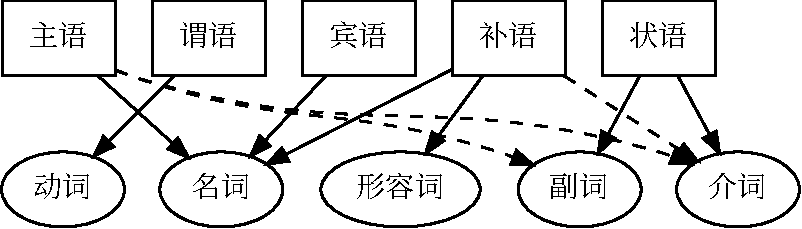
\includegraphics[width=0.7\linewidth]{svo.pdf}
  \caption{\label{fig:svo}句子成分与短语词类对应表}
  \capsource{注:虚线箭头表示在特殊情况下,主语可以是副词短语和介词短语,补语
    可以是介词短语。}
\end{figure}

本章谈的是比较根本的句型问题。虽然简单,却是了解英语语法必要的基础。读者在阅
读英语时不妨详加分析句型,触类旁通,相信会更有收获。

\section{Test}

\textbf{请判断以下各句属于五种基本句型中的哪一种?}

\begin{enumerate}
\item The magician moved his fingers quickly.
\item The police found the letter missing.
\item The police found the missing letter.
\item He ordered himself a steak and a bottle of red wine.
\item Don't you like dancing?
\item The President has gone abroad on a visit.
\item That sounds like a good idea.
\item The box feels heavy.
\item He told his guests a dirty joke at the party.
\item The people elected Bill Clinton President.
\item The child asks her mother a million questions a day.
\item Monkeys love bananas.
\item You can leave the door open.
\item The company has gone bankrupt.
\item Why don't you answer me.
\item I consider you a member of the family.
\item It never rains in California.
\item You 'll look better with these designer glasses on.
\item I can see better without these reading glasses.
\item Do you call me a liar.
\end{enumerate}

\chapter{名词短语与冠词}

名词短语是英语句子中不可或缺的元素。简单句的主语、宾语是它,补语也可以是名词
短语。\textbf{除了主语、宾语、补语这些主要元素外,介词后面所接的宾语也是名词短语},
所以名词短语使用的频率极高。不过名词短语很容易出错,尤其是\textbf{冠词}的部分,写作
时一不小心就会用错。一般语法书处理这个问题时,通常会列出一长串规则,再附注一
大堆例外,这种语法书,坦白说对于学英语的人并没有太大的帮助。本章就要和读者一
同来探讨名词短语,尤其是冠词的用法。本书中没有规则要背,自然也就不会有所谓的
例外。只要经由理性的探讨,便足以涵盖传统文法所有的规则,而且更深入、更灵活。

\section{名词短语}

首先,英语是一种拼音文字,和其他\textbf{拼音文字一样,用词尾的变化来表示单、复数}。
不仅如此,在名词短语的开头,还有一些符号来\textbf{配合标示该名词的范围},这种符号在语
言学上称为\textbf{“限定词”(Determiners)}。它与词尾的单复数符号互相呼应,共
同determine 名词的范围。冠词就是 Determiners 之中的一种。请看下面的例子:

\begin{table}[]
  \centering
  \begin{tabular}{ll}
    \textbf{a new book}         & 一本新书     \\
    \textbf{many good  students} & 许多好学生    \\
    \textbf{his beautiful wife} & 他美丽的妻子   \\
    \textbf{the best answer}    & 最好的答案    \\
    \textbf{those sweet roses}  & 那些芳香的玫瑰花
  \end{tabular}
\end{table}

这几个名词短语都是由三个部分所构成。第一个部分(a, many, his,the, those等)
就是\textbf{限定词},这个限定词决定第三个部分(book、students、wife等),亦即\textbf{名词}部分
的范围。中间的部分(new、good、beautiful等)则是\textbf{形容词},为依附在名词上的修饰
语,是可有可无的元素。

其实,\textbf{名词短语的这三个部分当中,每个部分都可以省略}。在 a new book中,即使拿掉
形容词,剩下 a book,这个名词短语还是正确的。同样地,在 the best answer 中如
果拿掉名词,剩下 the best 也一样是正确的。例如:
\begin{itemize}
\item Of these answers, this one is \unbf{the best}.

  在这些答案中,这个最好。
\end{itemize}

读者可以从此句中清楚了解 the best 就是 the best answer 的意思。甚至在those
sweet roses 中,可以把形容词和名词一起拿掉,只剩下those,仍是正确的名词短语。
比如说,你指着一些玫瑰花,对花店老板说:
\begin{itemize}
\item I want \unbf{those}.

  我要那种的。
\end{itemize}

老板就会知道你要的是什么。

\section{什么时候不需要用限定词?}

如果把 many good students 中的限定词 many 拿掉,剩下 good students,仍然是正
确的。但如果把 a new book 中的限定词 a 拿掉,只剩下new book,就变成一个错误的
名词短语,而这种错误在写作时偏偏常犯,所以我们有必要进一步加以讨论。

从语源学(etymology)的角度来看,冠词 a(n) 可以视为 one一字的弱化(reduction)
结果。也就是说,\textbf{a(n) 就代表 one的意思,只是语气比较弱。} a(n) 与 one同样都
是在交代\textbf{它后面所接的名词是“一个”的概念}。如果后面的名词不适合以“一个”来交
代,也就是不适合加a(n) 的话,就可把限定词这个位置空下来。例如:
\begin{itemize}
\item \unbf{Unmarried men} are a rare species these days.

  未婚男性目前是稀有品种了。
\end{itemize}

在名词短语 unmarried men中,只有形容词(unmarried)和名词(men)两个部分,而
没有限定词。这是因为men 一字已清楚表示名词是复数,自然不能再用 an来表示“一
个”,这时就可以把限定词省略。在 a new book 中,book是单数形态,因此要用限定
词来配合标示它。所以,如果只说 new book,就变成不完整的表示。

除了\textbf{复数}以外,\textbf{抽象名词}(如honesty、bribery)没有具体形状,不能以“一个”来
表示。物质名词(如water、food)虽然是具体的东西,可是\textbf{形状不固定},也不能以“一
个”来表示。\textbf{这些不能以a(n) 来引导的词就可以把限定词省略,即零冠词(the
  zero article)。}例如:

\begin{itemize}
\item  \unbf{Honesty} is not necessarily the best policy.

  诚实不一定是上策。

\item  \unbf{Fresh water} is a precious resource in Saudi Arabia.

  淡水是沙特阿拉伯的珍贵资源。
\end{itemize}

像 honesty 和 water 这些没有复数形态的词,都不适合加a(n)。我们可以这样说:如
果词尾加 ,则表示该名词为复数。如果前面加a(n),则表示“一个”,也就是单数如
果不能加 ,通常表示这个字没有办法数,自然也就不能说是“一个”了。这时候我们
就可以不用限定词。接着我们来处理一个比较复杂的问题:专有名词。

\section{专有名词与补语位置}

人名(如 Genghis Khan)、地名(如Taibei)等都是\textbf{专有名词。因为它所代表的对象
  只有一个,也不适合加a(n),所以可以不用限定词。}为什么只有一个的东西也不能
加 a(n)呢?因为如果用 a Genghis Khan 来代表成吉思汗,那么这里指的是 one
Genghis Khan(一个成吉思汗)的意思。亦即在此句中暗示有第二个成吉思汗存在,所
以才特别需要标示是“一个”。如果只有一个成吉思汗存在,就不必这样标示,只要
说Genghis Khan,大家也就知道在说谁了。加 a(n) 与加 是一体的两面,我们用这两
个符号分别来表示单、复数。\textbf{如果一个名词不能加 \emph{-s}(或者是作不规则复数变
  化),那么它也就不能加 a(n)。专有名词就是如此。}

要判断一个名词是否为专有名词,有时并不是那么容易。像 Sunday这种字,一个月中可
能会有四到五天,所以我们可以说:
\begin{itemize}
\item There are \unbf{five Sundays} this month.

  这个月有五个星期日。
\end{itemize}

这时候它就不算是专有名词。可是在一个星期中星期日只有一天,所以我们也可以说:
\begin{itemize}
\item I have an appointment on \unbf{Sunday}.

  我星期日有约。
\end{itemize}

这时它就是唯一的一天,也就算是专有名词。

实际上,可数与不可数只是根据“不同的\textbf{单位}来实现”(realized by different
lexical items),并无定然。并且是在世俗流变之中,如two cups of coffee在现实中
已可直说two coffees。




放在补语位置的专有名词最难以判断。补语和主语(或宾语)之间有同等的关系,\textbf{如
  果主语(或宾语)是专有名词(例如人名)的话,那么它的补语既然和它同等,便也
  会被当做是专有名词来使用,条件是在补语位置上的名词也必须具有“唯一” 的性
  质。}例如:

\begin{itemize}
\item Mr. Elson was \unbf{president} of the high school.

  埃尔森先生曾是这所高中的校长。
\end{itemize}

本句中 Mr.Elson 是人名,而且没有第二个存在,所以不能加 ,也不能加a,我们就
可以不用限定词。而在补语位置上的 president本来只是个普通名词,并不是只有这所
高中才有校长,而且这所高中的校长历来也不只埃尔森先生一人。因此,“校长”为普
通名词,而“埃尔森先生”为专有名词,两词性质本不相同。可是,因为在此句中“校
长”是埃尔森先生的补语,可以和埃尔森先生划上一个等号,所以可用专有名词来诠释
它。再者,当时这所高中校长一职确实只有埃尔森先生一人,因此也支持这个诠释。所
以president一词没有限定词。这就是把它当作专有名词的结果。再看下例:

\begin{itemize}
\item Some say he was \unbf{a better president} than Mr.Robert.

  有人说他当校长,比罗伯特先生干得更好。
\end{itemize}

在这个从属子句中,主语 he 就是埃尔森先生。president仍然是主语补语,可是这里就
要加 a了。为什么?因为在上下文中和罗伯特先生做比较,这么一来就有前后两任校长,
可以加 ,不是专有名词了。还有:

\begin{itemize}
\item  Mr.Elson is also \unbf{a member} of the Council of the city.

  埃尔森先生也是该城市政会委员。
\end{itemize}

本句中 a member of the Council 也是埃尔森先生的补语,类似 Council of the
city。可是高中校长同一时间只有一人,\textbf{市政会委员则有很多人},所以 a
member需要交代是“一名”,而非专有名词。

另外,当同位语是补语时,注意是否为专有名词,例如:

\begin{itemize}
\item Mattin Wales, \unbf{Head} of the football team, at the time, wore a
  mustache.

  马丁·韦尔斯,当时的足球队长,留有小胡子。
\end{itemize}

句中 Head of the football team 一般称为同位语,其实就是 who was Head of the
football team at the time 这个形容词从句的省略。其中 who代表马丁·韦尔斯,
而 Head则是主语补语,和马丁·韦尔斯是同等关系,所以仍然算是专有名词,不必用限
定词。

写主语补语时,要注意该补语是否为专有名词。写宾语补语时也是一样。例如:

\begin{itemize}
\item  Clinton made Gorle \unbf{campaign partner} of the Presidential election.

  克林顿选择戈尔为总统大选竞选搭档。
\end{itemize}

句中 campaign partner没有限定词,当专有名词使用。因为它是“戈尔”的宾语补语,
与其为同等关系。而副总统搭档只有一人,所以它便成为专有名词的用法。

\section{定冠词 the 的用法}

在语源学上,\textbf{the 可视为 that 或 those 的弱化形式。}而 that 或 those是指示限
定词,有明确的指示功能\footnote{此外,that, these或 those还可做指示代词。如 This is a
  question. }。所以定冠词 the也可以用同样的角度来了解:凡是上下文中有明指或暗
示时,也就是有“那个”的指示功能时,便要用定冠词the。请比较:

\begin{itemize}
\item  I need \unbf{a book} to read on my trip.

  我在旅途中需要带本书读。
\item  I have finished \unbf{the book} you lent me.

  我已把你借给我的书读完了。
\end{itemize}

在第一句中,a book 只是 one book 或 any book,并没有特别指定是哪一本。在第二
句中,the book 就是 that book,特别指出是“你借我的那本”。因为明指出来,所以
要用定冠词。请再比较:

\begin{itemize}
\item  \unbf{Modern history} is my favorite subject.

  现代史是我最喜欢的科目。
\item  \unbf{The history of recent China} is a sorry record.

  中国近代史是部伤心史。
\end{itemize}

第一句 modern history 一词中,history 是抽象名词,不可数,因而没有a。而在形容
词位置上的 modern 只是附在 history上的修饰语,并不算明确的指示,所以不必
加 the。第二句中 the history of recent China (中国近代史)则有 of recent
China附在后面,用来指出“那一段”历史。因为有这种指示性,所以必须在前面加上定
冠词the,但也不要死背前、后修饰语的差别。再看看下面这一组例子:

\begin{itemize}
\item  He should be home; I saw \unbf{a light in his house}.

他应该在家;我看见他家亮灯了。

\textbf{;} 用以连接两个以上独立句子,但各句子之间又有比句号紧密的关系;或者用以分隔
并列,但范畴略有差别的部分。如On our vacation, we visited London, England;
Paris, France; Berlin, Germany; and Rome, Italy.

\item  Turn off \unbf{the portal light}.

把门口的灯关掉。
\end{itemize}

第一句中虽然 a light 后面有 in his house来修饰,可是一栋房子中电灯可能有数十
个,如果看到有一个是亮的,仍然只能算是one light,而不是 that light 。所以 in
his house虽然放在后面,但并不算是明确的指示,仍然要用 a light。相反的,在第二
句中,叫人把大门口的灯关掉,在 the portal light一词中的portal,虽然是附在名词
前面的形容词,可是有明确的指示功能,因为门口的灯通常只有一盏,所以已经指明了
要关哪一盏灯,这时就要用the light。总之,不必死背,但要先了解 a(n) 是来自
于 one(一个),the则是来自于 that/those(那个),再逐一判断。

另外,如果上下文中没有明确指出来,但有\textbf{清楚的暗示},仍然要用定冠词the。例如,
先生对太太说:

\begin{itemize}
\item  I'm going to \unbf{the office} now.

  现在我要去办公室。
\end{itemize}

虽然 the office后并没有明指,可是太太知道,就是老公上班的办公室,这时还是要
用 the。再看下例:

\begin{itemize}
\item  Do you mind if I open \unbf{the window}?

  我可以把这扇窗户打开吗?
\end{itemize}

当有人在公共汽车上向你这么说时,虽然在 window前后没有指示性的字眼,可是对话的
情境清楚暗示“就是你旁边这扇窗户”,所以这时候还是要用the 。如果用 a,就变
成:

\begin{itemize}
\item  Do you mind if I open \unbf{a window}?

  我可以打开一扇窗户吗?
\end{itemize}

这时的意思便成为 any window,也就是对方要在整个公共汽车数十扇窗户中,随便挑一
扇来打开,却先来征求你的同意。虽然这不是不可能,却是很奇怪的讲法。

\section{定冠词与专有名词}

\textbf{专有名词的定义是:只有一个对象存在的名词},像 Genghis Khan 和 Taibei等。既然只
有一个对象存在,就没有“这个”、“那个”的分别,也就\textbf{不能加定冠词the}。如果你
说 this book,则暗示还有 that book 的存在,这时就需要指明是this book,也就
是 the book。像 Taibei这种字就不能这样使用。所以,专有名词和定冠词是有冲突、
且不能并存的。如果加了the,就表示这个东西有两个以上,也就不是专有名词了。例
如:

\begin{itemize}
\item  This is not \unbf{the John Smith} I know.

这不是我所认识的约翰·史密斯。
\item  This is a photography show of \unbf{the Taibei} 50 years ago.

这是表现 50 年前的台北的摄影展。
\end{itemize}

第一句暗示还有另一个约翰·史密斯存在,或是他有另外一面,是我所不认识的。这时
有两个约翰·史密斯存在,所以“约翰·史密斯”就不再是专有名词,可以
用this 或 that 来区分,这也就是为什么写 the John Smith的原因了。还有,“50年
前那个台北”这句话暗示和今日台北不同了,有两个台北。这时台北也就成了普通名词,
可以指来指去,所以要用the Taibei 50 years ago 来表示。

最后,在许多语法书上被列为例外,并要求学生背下来的东西,其实都非例外,反而都
是很容易了解的。比如,\textbf{一般语法书列出海洋、河流、群岛、群山、杂志名、船名等
  等,说这些是“要加定冠词的专有名词”,是例外。}但是,这种说法并非完全正确。
首先,这些清单并不周全。而且,大部分的人不是懒得背,就是背不下来。死背不但不
能变通,一碰到变化还是不会。现在我们就来看看这些所谓的例外:

\begin{longtable}[]{@{}ll@{}}
  \textbf{the Pacific (Ocean)} & 太平洋 \\
  \textbf{the Atlantic (Ocean)} & 大西洋 \\
  \textbf{the Indian Ocean} & 印度洋 \\
  \textbf{the Mediterranean (Sea)} & 地中海 \\
  \textbf{the Dead Sea} & 死海 \\
\end{longtable}

在“太平洋” the Pacific (Ocean) 一词中,Pacific是放在形容词的位
置,\textbf{字尾 \emph{-ic} 是明显的形容词字尾}。在名词位置上的 Ocean其实是\textbf{普通名词}(世
界上有三个洋。只要有两个以上就不算是专有名词),在此被省略掉。所以\textbf{定冠词the
  是配合后面的普通名词 Ocean},指出“叫做 Pacific的那个洋”。这是规规矩矩的用法,
完全没有例外。在三大洋中只有印度洋不适合省略,因为the Indian 可能会被误解
为“这名印第安人”。同理, the Mediterranean (Sea) 是普通名词 the sea 加上形
容词Mediterranean,也不是例外。“地中海”可以省略sea,因为省略之后仍然够清楚。
但“死海” the Dead Sea就不能省略,否则会被误会为“死人” the dead people。再
看下面的例子:

\begin{itemize}
\item  the Philippine Islands → \unbf{the Philippines}

菲律宾群岛
\item  the Alp Mountains → \unbf{the Alps}

阿尔卑斯山
\end{itemize}

这两个复数的“群岛” Islands、“群山” Mountains,也是普通名词。可是名词部分
被省略掉,以形容词位置取代之,并且把复数的  移到前面来。这也不是例外,只是
很合理的\textbf{省略方式}罢了。同样的:

\begin{longtable}[]{@{}ll@{}}
  \textbf{the Mississippi (River)} & 密西西比河 \\
  \textbf{the Titanic (Ship)} & 泰坦尼克号 \\
  \textbf{the Hilton (Hotel)} & 希尔顿饭店 \\
\end{longtable}

如果把这些名词短语的第三个部分还原,即可看出\textbf{它们的名词位置都是普通名词,所以
  都可以加冠词。}而所谓的专有名词都是放在形容词位置的修饰语,所以并不是什么例外,
请看下面的例子:

\begin{longtable}[]{@{}ll@{}}
  \textbf{the United States} of America& 美国 \\
  \textbf{the United Nations} & 联合国 \\
\end{longtable}

这两个例子中,在名词位置的其实都是普通名词(States,Nations),皆可加冠词。只有
America 这个名词短语是专有名词,所以前面没有加冠词。

以上的叙述中,重要观念有三:

\textbf{一、名词短语包括限定词、形容词、名词三个部分。任一部分都可能省略。}

\textbf{二、如果名词短语中不用限定词,是因为该名词不适合加 a(n)。}

\textbf{三、a(n) 是 one 的弱化结果,而 the 是 that/those 的弱化结果。}

这些观念都很容易理解,不必死背,而且可以充分诠释传统语法的规则与例外,如果多
加观察,以后在写作时,就可避免名词短语或冠词方面的错误。

冠词的问题基本上是写作时容易碰到的问题,阅读时要多加观察。在看文章的时候请留
心名词短语,尤其是冠词的用法,就是最好的练习。

\section{Test}


\textbf{请选出最适当的答案填入空格内,以使句子完整。}

\begin{enumerate}
\item The carpenter repaired \ttu.
  \begin{tasks}(2)
    \task the table's legs
    \task table's legs
    \task legs of the table
    \task the legs of the table
  \end{tasks}

\item Mr. Smith has three \ttu under his name.
  \begin{tasks}(2)
    \task shoe stores \task shoes stores \task shoe store \task shoestores
  \end{tasks}

\item The house sits on a \ttu road.
  \begin{tasks}(2)
    \task twelve feet in width
    \task of twelve feet
    \task twelve-foot-wide
    \task twelve-feet
  \end{tasks}

\item These men and women are all \ttu .
  \begin{tasks}(2)
    \task language's teachers \task languages teachers
    \task language teachers \task languages' teacher
  \end{tasks}

\item He ordered  \ttu for breakfast.
  \begin{tasks}(1)
    \task orange juice, bread and butter, coffee, and bacon, and eggs
    \task orange, juice, bread, and butter, coffee and bacon and eggs
    \task orange juice, bread and butter, coffee, and bacon and eggs
  \end{tasks}

\item The prime minister is the real ruler and the prince is merely \textbf{a} \ttu .
  \begin{tasks}(4)
    \task little
    \task small
    \task nobody
    \task none
  \end{tasks}

\item Living in the city, he was always being annoyed by noises of  \ttu .
  \begin{tasks}(2)
    \task one sort of other
    \task one sort of the other
    \task one sort or another
    \task one or others sorts
  \end{tasks}

\item Writing is one thing and talking is quite \ttu .
  \begin{tasks}(2)
    \task the other
    \task another
    \task others
    \task the others
  \end{tasks}

\item The majority of the Members of Parliament are men, but there are  \ttu  women, of course.
  \begin{tasks}(2)
    \task few
    \task little
    \task any
    \task quite a few
  \end{tasks}

\item  \ttu  is what he said: Don't go out!
  \begin{tasks}(4)
    \task This
    \task That
    \task The
    \task These
  \end{tasks}

\item Whether you serve coffee or tea doesn't matter;  \ttu  will do.
  \begin{tasks}(4)
    \task any \task either \task some \task all
  \end{tasks}


\item As we have finished the first chapter, now we will read  \ttu .
  \begin{tasks}(2)
    \task second \task the second \task second one \task the two
  \end{tasks}

\item \textbf{He has two daughters; one is a singer and \ttu  an actress.}
  \begin{tasks}(2)
    \task another \task other
    \task the other \task the others
  \end{tasks}

\item He asked if eighty dollars was enough, and I said that  \ttu twenty would
  do.
  \begin{tasks}(2)
    \task more \task another \task other \task the other
  \end{tasks}

\item Mary Kurt, \ttu  of the troupe, was strongly against smoking.
  \begin{tasks}(4)
    \task alto \task the alto \task an alto \task altos
  \end{tasks}

\item This kind of ball-pen holds  \ttu ink than that.
  \begin{tasks}(4)
    \task less \task fewer \task much \task little
  \end{tasks}

\item \textbf{John works harder than  \ttu boy in his class.}
  \begin{tasks}(2)
    \task all other \task any other \task all the other \task any
  \end{tasks}

\item I was told to take the pills  \ttu six hours.
  \begin{tasks}(2)
    \task each \task every \task other \task the other
  \end{tasks}


\item The man was badly wounded, but there could still be  \ttu  hope.
  \begin{tasks}(4)
    \task little \task few \task a little \task a few
  \end{tasks}

\item  \ttu  these people are going to the concert.
  \begin{tasks}(2)
    \task The most \task Most of \task Most \task Almost
  \end{tasks}

\end{enumerate}

\section{Answer}

\begin{enumerate}


\item (D) 所有格有两种表示方式:人与其他生物可用 's 的形式,无生物则用 of... 的
  介词短语形式来表示。本题的 table 是无生物,故只能从 C 和 D 之间选择。因为
  有 of the table 修饰前面的 legs,表示出来是“哪些”脚,所以要有定冠词 the。

\item (A) 复合名词,前面的 shoe 放在\textbf{形容词位置},只能用单数。后面的 store 要用
  复数,因为有限定词 three。D 的 shoestores 是错误拼法,两个词不能连起来。

\item (C) 冠词(a)与名词(road)之间是形容词位置,而且只能放单词,不能放短
  语\footnote{或许有人会写 a well paved road,但是严格的编辑会建议改为 a well-paved
    road,这样便于阅读。冠词和名词中间插入太多的词而不用hyphen/dash连接的话,
    会变得难读},故从 C 和 D 来选。既然是形容词,没有复数可言,故排除掉 D。

  另外名词+名词用于\textbf{测量},第一个名词前有一个数字。这个数字通常用连字符(-)
  连接到第一个名词上。请注意,在这些情况下,第一个名词通常是单数形式。

\item “语言教师”是复合名词,故由 B 和
  C 之间来选。前面 language 的位置是形容词位置,没有复数,故选 C。

\item bread and butter(奶油吐司)是一种食品,两个词都不可数,不需要限定词,构成
  一个名词短语,因而中间不能有逗号。bacon and eggs (火腿蛋)亦然。这里
  的 bacon 不可数,eggs 是复数,亦不需要限定词。

\item \textbf{(C)nobody 意为“无名小卒”时应作普通名词看待,可加冠词 a。A 和 B 都是形
    容词,不应置于冠词 a 后面当作名词用。}none 是 no one 的复合字,其中
  的 \textbf{no 就是限定词},所以前面不能再加冠词 a。

\item (C) one sort or another 表示 one sort or another sort,是一个常用的短语,
  意为“各种各样的”。

\item (B) 以 another(后面省略 thing)和 one thing 相对,可以表示“不同的两件
  事”,也是常用短语。

\item (D) C 的 any 只适用于否定句或疑问句。肯定句中的 any 要解释为“任何”,在此
  亦不适合。B 的 little 要配合不可数名词才能用。在 A 与 D 之间,few 是否定的
  意味,a few 才能表示肯定,而 quite a few 则是加上强调语气的副词 quite 来表
  示“还不少”。上下文要求肯定语气(由连接词 but 可看出),故选 D。

\item (A) 用来表示上文讲过的一句话,可以用 this 或 that 作代名词。例如:There's
  going to be a raise. Isn't this(或 that) great? 可是,如果代表下文要说的
  一句话,就只能用 this。

\item (B) 两者(coffee,tea)之间任选其一,应用 either,三者以上才用 any。

\item (B) the second 代表 the second chapter,与上文的 the first chapter 对称。

\item (C) 上文有交待一共是两个女儿,除去唱歌的那个,剩下的“那一个”是演员。句意
  中已指明哪一个,所以要用定冠词。the other 后面省略掉 is。

\item (B) 80 元当中已有四个 20(或四张 20 元钞票)了,所以说“再来一个 20(another 20)就够了。”意思是凑成 100。

\item (A) 空格位置是主语 Mary Kurt 的同位语,这个位置倾向于当专有名词看待。再加
  上这个乐团的女低音只有一人,符合专有名词的要求,因而不用冠词

\item (A) ink 不可数,故可排除 B。再从 than that 来看,应是比较级,故排除 C 和 D。

\item (B) 空格后面的 boy 是单数,所以排除复数的 A 和 C。英语的比较级要求较严格:
  只能说比班上“别的”同学用功,不然会造成“包括比自己用功”的语病,所以要
  有 other 一词来限定范围。

\item (B) 多久一次,像 every day,every week,every two months,every
  century(相当于 every hundred years)—样,要用 every 这个限定词来表
  示。six hours 固然是复数,可是像 hours,miles,pounds 这种代表“单位”的字
  眼也可以当单数使用,例如:Three miles is a long way to walk. 所以 every
  six hours 并无冲突。

\item (C) hope 不可数,所以从 A 和 C 来选。上下文要求用肯定语气:“还有希
  望”(从连接词 but 可以看出),所以用表示肯定的 a little。如果用 A,成
  为 little hope,只能表示否定语气:“希望渺茫”。


\item (B) 空格后面有完整的名词短语,已经有限定词 these,所以不能直接再加限定
  词 most 在前面(most 在此并非表示“最”的副词,而是表示“大部分”的限定词),
  只能用介词 of 隔开。而且 most 在此既非一般解释为“最”的最高级,前面也就
  不应用定冠词 the。

\end{enumerate}

\chapter{动词时态}

英语动词时态的变化,在学校里可能要花一个学期才学得完。语法书上也是洋洋洒洒一
大堆公式,好像非常复杂。其实,如果在句型诠释上稍微变通一下,时态问题是很容易
理解的,而且只需要了解两种状态:\textbf{简单式与完成式},就能充分掌握所有的时态变化。
本章我们就要在短短几页中,将所有的时态问题都解说完毕。

首先,在现代语法中,\textbf{时间(time)}和\textbf{状态(aspect)}是分开处理的。时间观念
(现在、过去、未来)非常简单,状态的观念就比较麻烦,如果再把\textbf{主动、被动语态
  (voice)}加进来,变化就更多了。以简驭繁的办法是:\textbf{把be动词(助动词)当做
  动词,其后的分词则视为形容词补语。}动词短语长的时候,里面一定会有be 动词,
如果把 be 动词抽离出来当做动词看待,那就只剩下\textbf{用 be动词写的简单式,以及
  用 have been写的完成式两种状态。}分词则可视为形容词补语,不放在动词短语里面,
如此一来整个时态的问题就会简单化,我们只要弄清楚什么是简单式,什么是完成式就
可以了。

\section{简单式}

简单式的动词可以清楚交代此动作是发生于哪个\textbf{时段}。而与它搭配的\textbf{时间副词}通常会明
确标示出一个时段。也就是说:简单式的时间是括弧的形状,我们可以用括弧把简单式
的时间括起来。在以下的叙述中,我们就以括弧来表示简单式中所描述的时间,这个括
弧大小不拘,可以小到一个点,也可以大到无限,可是必须标示得很明确。现在来看看
几个例子,请注意观察动词时态与时间副词之间的关系:

\subsection{过去时间}

\begin{itemize}
\item The U.S. \unbf{established} diplomatic relations with the P.R.C. \unbf{in 1979}.

  美国与中华人民共和国于 1979 年建交。
\end{itemize}

此句中,以 in 1979 来修饰动词establish(建立)的时间,表示美国与中华人民共和
国建交发生在这段时间内,所以我们可以用括弧将in 1979 括起来。而这个括弧在 now
的左边,属于过去时间,所以动词用established,是过去时间的简单式。

\begin{itemize}
\item  The movable print \unbf{was} introduced to England in \unbf{1485}.

  活版印刷于 1485 年被引进英国。
\end{itemize}

此句中,把 be 动词当动词看,他的时间副词 in 1485 也是一个括弧,在 now的左边,
同样是过去时间的简单式,所以\textbf{动词是was},意思是说:活版印刷引进英国这件事情
是发生在那个括出来的时段中。\textbf{过去分词introduced 当作形容词补语看待},过去分词
字尾 \emph{-ed}视为一个表达被动意味的形容词字尾。be动词是一个没有意义的连缀动词,
用来连接主语“活版印刷”和补语“被引进(到英国)”。be动词虽然没有意义,不需
要翻译,可是它是动词,必须以它来\textbf{决定时态},所以用was 的过去简单式出现。

\begin{itemize}
\item  I \unbf{was} visiting clients \unbf{the whole day yesterday} .

  昨天一整天我一直在拜访客户。
\end{itemize}

同样地,把 be 动词视为动词看待会比较简单。时间副词 the whole day yesterday 的
性质和 in 1979是相同的:都是一个过去时间的括弧。所以,动词时态也是一样的:都
是过去简单式:was。be动词后面 visiting clients这个部分可视为一个现在分词的短
语,做为形容词补语来形容主语。\textbf{现在分词表示一种持续性,相当于中文
  的“正在”、“一直”的口吻。}be动词不必翻译,因为它是一个没有意义的连缀动词,
连接主语“我”和补语“一直在拜访客户”。be动词只要负责交代时态就好。而“昨天
一整天”是一个过去的时间,所以用was,也就是过去简单式。

\begin{itemize}
\item I \unbf{was} watching TV \unbf{when I heard the doorbell} .

听到门钤响的时候,我正在看电视。
\end{itemize}

这个句子的时间副词“我听到门铃响的时候”,是指门铃响起来那一刹那,所以是很短
的\textbf{一瞬间}。上面说过简单式要括出动作发生的时段,而这个括弧可大可小。在when I
heard the doorbell中,这个括弧就是最小的一个点:听到门铃的那一刹那,所以动词
仍然要用简单式。将be 动词当做动词看待,要用过去简单式was。而那时候“我”“正
在看电视”。主语与补语 watching TV 之间用 be动词连起来,将 watching TV 视为形
容词短语。

\begin{itemize}
\item  The witness \unbf{was} being questioned in court \unbf{when he had a heart attack} .

证人心脏病突发时,他正在法庭上被质询。
\end{itemize}

此句中,时间副词 when he had a heart attack指的是他心脏病突发的瞬间,是一个最
小的括弧。而 had表示这个时间是过去的时间,所以 be 动词用 was来表示过去简单式。
主语是“证人”,be 动词后面的部分当形容词补语看待,有being 和 questioned 两个
分词,都视为形容词。be 动词是没有意义的,所以being 的存在主要意义不在 be,而
在字尾 \emph{-ing}。这个字尾表示“\textbf{正在}”,所以being 只要解释为“正在”就可以了。
过去分词 questioned也当形容词看,可是过去分词字尾 \emph{-ed} 表示\textbf{被动},配
合 question就解释为“被质询”,所以,being questioned解释为“正在被质询”,用
来做为主语“证人”的补语。动词 was还是过去简单式。

两种一般过去时形式之间通常存在的是\textbf{时间顺序}关系;过去进行时和一般过去时形式
之间存在的则是\textbf{时间内包关系 (TIME-INCLUSION)}:
\begin{itemize}
\item When we \unbf{arrived}, Jan \unbf{made} some fresh coffee.

  时间顺序,到达后煮咖啡。

\item When we \unbf{arrived}, Jan\unbf{ was making} some fresh coffee.

  时间内包,到达时正在煮咖啡,到达的一瞬内包在煮咖啡期间。
\end{itemize}

\subsection{现在时间}

如果时间副词是 now,或是以 now为中心的或大或小的括弧,就要用现在时间的简单式。
从前语法书中列出规则:真理以及事实要用现在简单式表示。其实这也没什么好背的。
因为,只有在以now为中心的括弧,可以大到涵盖过去未来,才可以用来表示不变的真理。
请看下面这些例子:

\begin{itemize}
\item Huang \unbf{pitches} a fast ball. Li \unbf{swings}. It \unbf{looks} like a hit. The shortstop
  \unbf{fails} to stop it. It'\unbf{s} a double!

  黄投出快速球,李挥棒,好像是安打,游击手没有拦到球,是二垒安打!
\end{itemize}

播报运动比赛时,常会用到一连串的现在简单式。像这些句子,虽然没有交代时间副词,
可是很明显每一句都是现在发生的,也就是now。播报员所播报的\textbf{一直是现在这一
  刻}所发生的事情,所以就是 now这一瞬间,也就是最小的括弧。只要是括弧就是简单
式,所以是现在简单式。

其实,\textbf{一系列瞬息动作使用现在简单式,为事件赋予了画面动感。}

\begin{itemize}
\item  Bush \unbf{is} the U.S. President.

  布什是美国总统。
\end{itemize}

布什是现任美国总统,可是几年前他不是,几年后他也可能不再是。这个句子的时间是
一个以now 为中心的括弧,所以用现在简单式。

\begin{itemize}
\item  All mothers \unbf{love} their children.

  天下的妈妈都爱自己的小孩。
\end{itemize}

天下的妈妈没有不爱小孩的。这是古今皆然,以后也不会改变,所以这是以 now为中心
的一个\textbf{极大的括弧}。不论大小,只要可以用括弧表示,就是简单式,所以动词用现在简
单式的love。

\begin{itemize}
\item  7-ELEVEN \unbf{is} selling big cokes at a discount \unbf{this month}.

  统一超市这个月大杯可乐打折。
\end{itemize}

把 be 动词当动词看,时间副词 this month 是以 now为核心的一个括弧,所以用现在
简单式is。可乐打折,是正在持续中的活动,所以用 selling big cokes,\textbf{以现在分
  词片词做补语来强调持续性}。

\begin{itemize}
\item According to the NASA survey, the ozone layer \unbf{is} being depleted.

  根据美国国家航空和航天局的研究,臭氧层正在被消耗中。
\end{itemize}

这是一个以 now 为中心的较大的括弧,所以动词用现在简单式 is,而 being
depleted 当做补语看待。being 只有词尾 \emph{-ing}有意义,解
释“正在……”。depleted中过去分词的词尾 \emph{-ed}有被动的意思,所以解释
为“被消耗”。两词合在一起,being depleted就是“正在被消耗”当形容词补语看待,
形容主语“臭氧层”。现在简单式的动词is 则不需要翻译。

\subsection{未来时间}

未来时间的简单式,只是把括弧放在 now的右边,其他的原理则完全相同。至于里面会
有一些牵涉到语气问题的变化,在本章会做初步的解说,详细的说明则留待第九章再作
讨论。

\begin{itemize}
\item  There \unbf{will be} a major election in \unbf{March}.

  三月将有一次大选。
\end{itemize}

时间副词 in March是一个未来时间的括弧。只要可以括出时间来就是简单式。未来的事
情还没发生,尚未确定,所以要加一个助动词will 在前面,意思是“到时候会”。

\begin{itemize}
\item  Don't call me at six tomorrow. I'\unbf{ll still be} sleeping
  \unbf{then}.

  不要在明天六点时打电话给我。我那时还在睡觉。
\end{itemize}

明天六点,是六点整那一刻,所以是一个最小的括弧,因为是在 now的右边,所以要用
未来简单式。把 be 动词当动词看,未来简单式 will be后面的 sleeping 就要当形容
词补语。而词尾 \emph{-ing} 表示持续性。所以 sleeping是“在睡觉”,用来形容主语“我”。
动词 will be 当中,连缀动词 be没有意义,只要解释 will 的部分“会”即可。

\begin{itemize}
\item  The building \unbf{will be} razed \unbf{next month}.

  这房子下个月拆除。
\end{itemize}

时间副词 next month 是一个未来时间的括弧,所以动词用未来简单式:will be。后面
的razed(被拆除)是过去分词,当形容词补语看待,形容主语“房子”。

\section{完成式}

另一种主要的状态是完成式。\textbf{相对于简单式用括弧形状来表达时间,完成式则是以箭
  头形状来表达时间,表示动作的截止时间。}从功能上来看,\textbf{简单式是交代动作发生
  的时段;而完成式并不对动作发生的时段作明确的交代,只表
  示“曾经”、“做过”的意思。}请看看下面的例句。

\subsection{现在时间}
\begin{itemize}
\item  I'm sure I \unbf{have seen} this face somewhere.

  我肯定曾经见过这张脸。
\end{itemize}

主要从句 I'm sure 的动词 am表示是现在时间,除此之外,没有时间副词交代是什么时
候“看到”这张脸的,只知道一定有见过。也就是说,“看到”的动作没有明确括出来
是哪一个时段发生的,只有一个箭头的形状,表示截止时间是现在。在这一刻以前看到
过都算数,以后才要去看则不算数。这就是现在时间完成式的条件,所以用have
seen(看过)。

\begin{itemize}
\item We \unbf{have been} working overtime \unbf{for a week} to fill your order.

我们
  连续加班一个星期赶出你订的货。
\end{itemize}

把 be动词当做动词看,那么再复杂的动词时态也只剩下两种变化,不是简单式就是完成
式。这里用完成式,因为时间副词for a week是“到现在,算算有一个星期之久了”,
这时候重点在于“算到现在已经有……了”,所以强调的是截止时间,是箭头形状的时
间,要用完成式“已经”来配合,所以动词用have been。后面的补语 working是现在分
词,表示\textbf{持续性},也就是“一直在加班”,用来形容主语“我们”。动词have
been 是 be动词,不必翻译,只要解释完成式的部分“已经”和时间副词“有一个星
期”就可以了。

\begin{itemize}
\item  The house \unbf{has been} redecorated twice \unbf{since they moved in}.

  打从他们搬来算起,这栋房子已经被装修过两次了。
\end{itemize}

这个句子的时间副词 since they moved in(打从他们搬来算起)虽然是表示开始计算
的时间,可是语气的重点是“算到现在是多久”,所以仍然用完成式has been。补语部
分 redecorated是过去分词,要加上被动的解释,成为“被装修”,来形容主语“房
子”。

\subsection{过去时间}

如果没有特别交代的话,一般说“有……过”就是“到现在有……过”,所以都是现在
完成式。用过去完成式时则要有一个过去的截止时间,也就是箭头指在一个过去时间,
在那之前就“有……过”。

\begin{itemize}
\item  Many soldiers \unbf{had died} from pneumonia \unbf{before the discovery of penicillin}.

  发现盘尼西林以前,已经有很多士兵死于肺炎。
\end{itemize}

盘尼西林在 1928 年发现,可是这个句子的时间副词不是 in 1928一个括弧,而
是 before the discovery of penicillin,也就是 \textbf{before 1928,是一个以 1928 年
  为截止时间的箭头形状,所以要用过去时间的完成式 had died。}换句话说,这个句
子说到的士兵从古罗马时代,一直到一次大战都可以算在里面,但1928 年之后的就不算
了,因为盘尼西林已经发现了。这就是过去完成式的条件。

\begin{itemize}
\item  I \unbf{had been} smoking three packs of cigarettes a day \unbf{before I decided to quit}.

  我决定戒烟之前,每天要抽三包烟。
\end{itemize}

decided 是过去时间,而时间副词 before I decided是“在我决定之前”,所以不是括
弧而是箭头,以 decided为截止时间。这就得用过去完成式 had been。补语 smoking
three packs是一个形容词短语,\textbf{-ing表示持续性,也就是每天都要抽三包烟,
  而且是“一直如此”,}用来形容主语“我”。


\begin{itemize}
\item  Japan \unbf{had not been} defeated yet \unbf{by the time Germany surrendered} unconditionally.

  到德国无条件投降为止,日本尚未被打败。
\end{itemize}

这个句子的时间副词是“算到德国投降为止”,所以是一个到过去时间截止的箭头。这
就是过去完成式。动词had not been 表示“尚未”,就是“已经”的相反。be动词仍不
必翻译。补语部分 defeated是过去分词,表示被动的形容词,“被打败”用来形容主
语“日本”。

\subsection{未来时间}

未来时间的完成式,只是把箭头所指的截止时间移到未来的一个点。观念上与现在、过
去时间的完成式完全一样。在写法上,因为是未来时间,所以动词前面加一个will 就可
以了。请看例句:

\begin{itemize}
\item  \unbf{Next April}, I \unbf{will have} worked here \unbf{for 20 years}.

  到四月,我在这里就工作 20 年了。
\end{itemize}

这个句子中有括出时间 next April,看起来好像要用简单式。可是另外还有一个时间副
词 for 20 years,是一个箭头。你不可能在四月这个月内替公司工作 20 年,所
以 next April 只是一个截止时间,表示“算到四月为止有 20年”来修饰动词,所以要
用完成式。动词前面加上will,表示到现在还没有,要到四月才“会”做满 20年,也就
是未来时间的完成式。

\begin{itemize}
\item  Come back \unbf{at 5:00}. Your car \unbf{will have been} fixed \unbf{by then}.

  五点再来吧!到时候你的车一定已经修好了。
\end{itemize}

你去修车厂拿车子,老板叫你五点再来。他的意思不是五点才要修你的车,而是说五点
以前就一定先修好了,等你来拿。真正修好的时间可能是四点,也可能是三点也说不一
定,反正不超过五点。这就是完成式的箭头形状时间;\textbf{截止时间在未来},所以用未来完
成式will have been。be动词没有意义,只要翻译时态“会已经”,来连接主语“车
子”和补语“被修好”(fixed)。

\begin{itemize}
\item \unbf{In two more minutes}, she \unbf{will have been} talking on the phone for
  three hours!

  再过两分钟,她就一直打了足足三小时的电话了!
\end{itemize}

这位小姐也真能讲话。动词是 be 动词,连接主语 she 和补语talking,“她一直
讲”,\emph{-ing}的字尾表示持续性,当形容词看。“再过两分钟”是未来的一个截止点,算
到那时候就有三小时了(for three hours),所以是完成式的箭头型时间,要用未来完
成式的动词 will have been,“会已经”(有三小时)。再和主语“她”与补语“一直
打”连在一起,意思就清楚了。

\section{结语}

英语的动词时态很复杂,可是也可以很简单,只要在句型上转个弯,换个角度来看,就
可豁然开朗。以上的探讨除了一些牵涉到语气的问题留待以后处理之外,已涵盖了传统
语法中所有的时态变化。

其中所牵涉的重要观念有以下几点:

{\bfseries 一、把 be 动词当动词看,句子就只剩两种状态:简单式与完成式。

  二、简单式是以括弧型的时间来表达。

  三、完成式是以箭头型的时间来表达。

  四、be动词后面的分词当作形容词补语。现在分词有正在进行的意思,过去分词有被动的意思。}


\section{Test}

\subsection{练习一}

\textbf{请选出最适当的答案填入空格内,以使句子完整。}

\begin{enumerate}
\item So far we \ttu nothing from him.
  \begin{tasks}(2)
    \task have been heard
    \task did not hear
    \task have heard
    \task have not heard
  \end{tasks}


\item At present a new road \ttu in that part of the city.
  \begin{tasks}(2)
    \task is building
    \task will be built
    \task will have built
    \task is being built
  \end{tasks}

\item Our city \ttu a great deal. It doesn't resemble the one of three years ago.
  \begin{tasks}(2)
    \task changes
    \task has changed
    \task is changing
    \task will change
  \end{tasks}

\item When Anna phoned me I had just finished my work and \ttu to take a bath.
  \begin{tasks}(2)
    \task was starting
    \task have started
    \task starting
    \task will start
  \end{tasks}

\item There \ttu some very bad storms recently.
  \begin{tasks}(4)
    \task is
    \task are
    \task have been
    \task have
  \end{tasks}

\item  The future price of this stock \ttu by several factors.
  \begin{tasks}
    \task is going to determine
    \task will determine
    \task will be determining
    \task will be determined
  \end{tasks}

\item The camera was invented in the 19th century. At that time, most photographers \ttu professionals.
  \begin{tasks}(2)
    \task are
    \task were
    \task have been
    \task had been
  \end{tasks}

\item The whole area was flooded because it \ttu for weeks.
  \begin{tasks}(2)
    \task rains
    \task has rained
    \task had been raining
    \task was raining
  \end{tasks}

\item By next Sunday you \ttu with us for three months.
  \begin{tasks}(2)
    \task will have stayed
    \task will stay
    \task shall stay
    \task have stayed
  \end{tasks}


\item \textbf{We could smell that someone \ttu a cigar.}
  \begin{tasks}(2)
    \task would be smoking
    \task was smoked
    \task had been smoking
    \task would be smoked
  \end{tasks}

\end{enumerate}

\subsection{练习二}

\textbf{请把括弧中的动词以适当的时态填入空格内,以使对话内容完整。}

item Boy: Do you want to go and see \textit{Gone with the Wind} with me tonight?

Girl: No! I \ttu (1. see) it.

Boy: Oh, really? When did you see it?

Girl: I \ttu (2. go) to see it the first day it was on-last Monday.

Boy: To tell you the truth, I have seen it too. In fact, I \ttu (3. see)it before you did.

Girl: That's impossible. I told you I saw it the first day it was on.

Boy: But it's the truth! I \ttu (4. see) it seven or eight years ago, the
last time that old picture \ttu (5. come) in town.


Girl: In that case, why did you ask me to go in the first place? Boy: Well,
I just \ttu (6. want) to go out with you tonight. Since you have seen the
picture, will you go to the baseball game with me instead?

Girl: I \ttu (7. guess) I will, if Father says Okay. But you will have to
pick me up at my place.

Boy: Great! I \ttu (8. see) you at 5:30 then. I'll bring my car.

Girl: But why 5:30? Why not seven o'clock?

Boy: Because the game \ttu (9. start) by then. These evening games \ttu (10.
begin) at 6:30, you know. Don't forget now, 5:30 at your place!

\section{Answer}

\subsection{练习一答案}

\begin{enumerate}
\item (C) so far(到目前为止)应用现在完成式,故排除过去式的 B。主语是 we,表示“我们听到”时应用主动态,故排除被动的 A。因空格后已有否定的 nothing,所以不选表示重复否定的 D。

\item (D) at present 表“现在”,应用现在式,故排除未来式的 B 和 C。主语 road 与
  动词 build 配合,应用被动态表示“被建造”,故排除主动的 A。答案 D 表示“现
  在正在被建造中”。

\item (B) “现在它和三年前已大不相同”,可以看出,空格那个 change 要表示的是从三
  年前到现在的改变,因此选择现在完成式 B。A 和 C 其实也没错,表示它“经常在
  变”,不过这两个答案与题目第二句的呼应不及 B 密切。D 的未来式则和题目第二句
  有较大的冲突。

\item (A) 从 when Anna phoned me 以及 I had just finished 可看出时间在过去,因此
  表示现在时间的 B 和未来时间的 D 都可排除。又,空格前面有对等连接词 and,要
  求对称。在 A 和 C 之中只有 A 是动词短语,可以和前面的动词短语 had just
  finished 对称。

\item (C) recently 表示“不久前到现在”,应用现在完成式。表示“有”的观念应用 There is/are 的句型,其现在完成式即是 have been(主语 storms 是复数)。

\item (D) 从 future price(未来价格)可看出时间在未来。主语 price 与动词 determine 配合应用被动态,这点从空格后面的 by several factors 亦可看出。唯一正确的被动态是 D。

\item (B) 从 at that time 可看出时间在过去(19 世纪)。因明确表示出那一段时间,
  应用过去简单式,故选 B。

\item (C) 从主要从句 was flooded 可看出,淹水是过去时间,而造成淹水的原因“下雨”,只能在淹水之前发生,所以该用过去完成式。

\item (A) next Sunday 表示未来时间,故排除现在时间的 D。然后介词 by 表示“到……为止”,应用完成式,因而排除简单式的 B 和 C。

\item (C) 主语 someone 和动词 smoke(有人抽雪茄)配合应用主动态,故可排除被动
  的 B 和 D。而 A 的 would be smoking 表示“将抽未抽”,如此则和 we could
  smell(已闻得到)有冲突,故选过去完成式的 C,表示在那之前已有人在抽,才会留
  下味道。Hide Answer

\end{enumerate}

\subsection{练习二答案}

\begin{enumerate}
\item have seen 看过,而不说何时看的,应用现在完成式。

\item went 既说出看的时间(last Monday),应用简单式。

\item had seen 时间是 before you did,只知在过去时间 you did 之前,未明言在何时,
  应用过去完成式。如果用 saw 也不算错,因为在 I saw 和 you did 之间有 before
  相连,清楚交待两个动作的先后,不必倚赖过去完成式来交待。

\item saw 因交待了“七八年前”,应用简单式。用 had seen 也不算错,这样的语气
  是“我看得比你早”,至于“七八年前看的”这点则在语气上不予强调。

\item came 因有 the last time 标出时间,应用简单式。

\item wanted 因为是回应 Why did you \ldots{} ?

\item guess 这是这位小姐说话时的猜想,时间就是 now,应用现在式。

\item will see 因为说出 at 5:30 的未来时间。

\item will have started 因为时间是 by then,也就是“到了那个时候”,老早开打了。
  没说几点开打,总之在那之前,这就是完成式。也可用 would have
  started,用 would 不是表示过去时间,而是表示非事实的假设,成为:“如果真的
  拖到七点才去的话,那就看不成了,非早点去不可!”这样的口吻。

\item begin 因为 \textbf{these} evening games 不只说今晚这场,而是“所有的晚场比赛都是”,
  也就是说包括今天的这一阵子都是如此,就得用现在简单式。
\end{enumerate}

\chapter{不定式}

\section{带to与不带to的不定式}

不带to的不定式中第一个动词用动词原形,因此很多人不知道不带to的不定式,只知道
动词原形。我觉得,为方便理解,最好还是将动词原形与不带to的不定式区分开为好。

\begin{description}
\item[动词原形] 动词的基本形式,可以通俗认为只用在\textbf{祈使句}。\textbf{既没有时态
  的标记,也没有体的变化。}
  \begin{itemize}
  \item \unbf{Come} here.

  \item Let us party.
  \end{itemize}

\item[不带to的不定式] 用在\textbf{情态助动词}(can, may, could等
  ),\textbf{感官动词}(see, hear, feel等),\textbf{使役动词}(let, make,
  have等)后面,采用动词原形形式。

\item[带to的不定式] to + 动词原形。可以\textbf{将其中的to理解为情态助动词功
    能},并常表示\textbf{有不确定性}。
\end{description}

不同于原形,两种不定式都\textbf{没有时态的标记,但有体的变化。} 如should/to write,
should/to be writing, should/to have written, should/to have been writing.

按这种方式理解,就可将带to与不带to的不定式融会贯通起来,不需背诵过多规则。

\section{to与助动词的共同点}

要了解不定式与助动词之间的关系,不妨先看一个例子:

\begin{itemize}
\item  I am glad \unbf{to know you}.

  很高兴能认识你。
\end{itemize}

这是一句简单的会话用语,读者应该都能脱口而出。可是如果追问下去:“为什么用不
定词to know you?”“为什么不能用动名词 knowing you?”恐怕许多读者就答不上来
了。(请不要回答“我背过”,或者“这是惯用法”、“这是短语”;语法要求理解,
不能打迷糊仗。)其实,只要了解不定式与助动词之间的关系,就可以了解这个不定式
是来自助动词的变化。怎么说呢?我们来看看这个例句还原成原状的样子:

\begin{itemize}
\item  I am glad \unbf{because/that I can know you}.
\end{itemize}

这句话可以进一步改写为下面这个类似的句子:

\begin{itemize}
\item  I am glad \unbf{because/that I am able to know you}.
\end{itemize}

由连接词 because 所引导的副词从句中,主语 I和前面主要从句的主语相同,是重复的
元素。动词 am 是个空的 be动词,没有意义。因此这两个元素(I am)都可以省略。可
是,副词从句中省略主语与动词之后,已经不成一个完整的从句结构了。如此一来,连
接词because 也就没有必要存在。剩下的不定式 to know 本身就带有 able to的暗示,
所以就变成:

\begin{itemize}
\item  I am glad \unbf{to know you}.
\end{itemize}

翻译成“很高兴能认识你”,是因为这个 to know 就是 able to know,也就是can
know 的变化。

从这个例子可以看出,不定式与助动词的关系极为密切,我们可以利用这层关系来练习
判断不定式的用法。首先,我们来观察一下不定式与助动词之间有什么共同点。

\subsection{后面都要用动词原形}

\begin{itemize}
\item I \unbf{will go}.

  我要走了。
\item I \unbf{want to go}.

  我想去。
\end{itemize}

\subsection{都有“不确定”的语气}

\begin{itemize}
\item He \unbf{is} right.

  他是对的。
\item He \unbf{may be} right.

  他可能是对的。
\item He seems \unbf{to be} right.

  他好像是对的。
\end{itemize}

第一句 He is right是确定的语气,把“他是对的”当作事实来叙述。一旦加上助动
词 may之后,就成了不确定的语气。所以第二句 He may be right只是一个推测,不是
事实叙述。第三句He seems to be right也是推测,不是事实叙述。这种不确定语气是
to与助动词之间一个很重要的共同点,可以用来判断何时该用带to不定式。

\subsection{都要用完成式来表达相对的过去时间}

助动词与不定式中的to本身都无法完整表达过去时间。如果你听到“哗啦哗啦”的声音从外面传来,可以说:
\begin{itemize}
\item It \unbf{must be} raining now.

  一定下雨了。
\end{itemize}

如果看到天上乌云密布,一副山雨欲来的样子,也可以说:
\begin{itemize}
\item It \unbf{may} rain \unbf{any minute}.

  随时都可能下雨。
\item It \unbf{might} even snow.

  说不定还会下雪。
\end{itemize}

这几个例子中,第一句的助动词 must 没有过去式的拼法。至于第二句、第三句的may
和might,咋看之下好像有现在式和过去式的区别。可是用在猜测语气中并不是如
此。It may rain any minute 是未来时态,It might even snow同样也是未来时态,这
时的 might 并不是 may的过去式,只表示比较保留、比较没有把握的猜测语气。所以,
不论像 must这类只有一种拼法的助动词还是像 may,might这类有两种拼法的助动词,
都只能用来猜测现在或未来时间的事情,\textbf{助动词本身缺乏表达过去时间的能力}。

如果你早上起来看到地上湿湿的,于是说:

\begin{itemize}
\item  It \unbf{must have rained} last night.

  昨晚一定下过雨。
\end{itemize}

\textbf{在猜测过去的事情时,助动词不论是 must、may 还是might,都只能表示语气强弱的
  差别,无法表达过去。}助动词后面要接动词原形,也不能用过去式,所以别无选择,
只好用\textbf{完成式}来表示过去,也就是must have rained 这种形态。就这点来看,不定
词仍然与助动词相同。

\begin{itemize}
\item  It \unbf{seems to have rained} last night.

  昨晚好像下过雨。
\end{itemize}

这个句子的动词 seems是现在式,表示“现在看起来”、“现在的推测”。可是推测的
事情是昨天晚上的事,是过去的时间,所以“下雨”应该是过去式,但是\textbf{to与助动
  词一样,本身缺乏表达过去的能力},后面都要接动词原形,也不能用过去式,所以
只能用\textbf{完成式}来表示过去,变成to have rained。这又是不定式和助动词的一个共同
点。

\subsection{所有重要的情态助动词,都可以改写为不定式}

请观察以下的对照:
\begin{table}[htbp!]
  \centering
  \begin{talltblr}[ caption = {情态助动词可改写为不定式(半助动词)},
    label = {tab:modalinf},
    ]{
      width=\linewidth, colspec={ccc},
      rowsep=2pt, colsep=4pt,
      row{1} = {c, font=\bfseries},
    }
  \toprule
  情态助动词 & 不定式\\\midrule
  must & have to \\
  should & ought to \\
  will/would & be going to \\
  can/could & be able to \\
  may/might & be likely/allowed  to \\
  \ul{be (just) going to} & be about to \\
  \bottomrule
  \end{talltblr}%
\end{table}

从以上四点来看,\textbf{不定式中的to与助动词其实是同一种东西的相互变化},凡是
不定式出现的地方,都可以看成是另外一个从句的省略:把主语省略,助动词改为to。

\section{不定式与动名词的区分}

传统语法所称的\textbf{动状词(Verbals)},包括现在分词(Ving)、过去分词(Ven)、动
名词(Ving)与不定式(to V)等等。其中\textbf{现在分词、过去分词是形容词类},不定式则
是“不一定什么词类”:它可以当名词、形容词、副词使用。这就产生了一些混淆点。
比如说,动词后面的宾语位置,必须用名词类。可是动名词和不定式都可以当做名词使
用(分词只能当形容词,可以不必考虑),到底应如何区分?这就要借助我们刚才的观察
了。现在来看看几个具有代表性的动词:

\subsection{plan}

\begin{itemize}
\item  \unct{They}{S} \unct{plan}{V} \unct{to marry next month}{O}.

  他们计划下个月结婚。
\end{itemize}

这个句子的 to marry next month 是 plan的\textbf{宾语},必须用名词类。那么为什么用不定
词 to marry,而不用动名词 marrying呢?因为 to marry next month 就是 (that)
they will marry next month的变化。marry 是计划中的事情,下个月才要发生,是\textbf{未
  来式}。再把 they will marry 改成 they are to marry。这时候,如果把重复的主
语 they 和空的 be动词 are 省略掉,就成了不定式 to marry。

\subsection{avoid}

\begin{itemize}
\item  \unct{I}{S} \unct{avoid}{V} \unct{making the same mistake twice}{O}.

  我避免犯同样的错误。
\end{itemize}

这里用 making 比用 to make 恰当,因为 to make 是 will make的省略,既然
是“\textbf{避免}”,后面又用 will make(将要做),意思就变得不清楚了:

\begin{itemize}
\item  \unct{I}{S} \unct{avoid}{V} \unct{something}{O}.
\item  I will make the same mistake twice.
\end{itemize}

一般语法书中规定 avoid后面要用动名词,这是因为\textbf{四种动状词中,只有动名词和不
  定词可以做名词类使用},也就是说:只有这两个可以当avoid 的宾语。如果用不定
词 to make,则带有 I will make这种\textbf{未来式}的涵意,与 avoid这种具有\textbf{否定}意思的动
词并不适合并列,所以只剩下动名词 making是唯一的选择了。

\subsection{hate}

\begin{itemize}
\item  \unct{I}{S} \unct{hate}{V} \unct{to say this}{O}, but I think you're
  mistaken.

  对不起,你错了。
\end{itemize}

在这个句子中,hate 固然也是否定的意思,可是后面却要接 to say,这是因为to say
是 I have to say,也就是 I must say的变化,表示“虽然很不愿意说,可是我\textbf{不能
  不}说。”

\subsection{like/dislike}

\begin{itemize}
\item \unct{I}{S} \unct{like}{V} \unct{to be the first}{O}.

  我喜欢排第一。
\item \unct{I}{S} \unct{don't like}{V} \unct{to wait too long}{O}.

  我不喜欢等太久。
\item \unct{I}{S} \unct{dislike}{V} \unct{standing in long lines}{O}.

  我讨厌排队。
\end{itemize}

第一句中的 to be,可以视为 I can be 的变化。第二句中的 to wait 可以视为I
will wait 的变化,它可以做为 like 的宾语,成为 like to wait(愿意等),或变成
否定句 don't like to wait(不喜欢等),这些都可以使用不定式。只有第三句,动
词\textbf{dislike(不喜欢)本身是否定的,后面就不适合接 I will stand in long
  lines(愿意排队)}。而且 dislike 不像 hate,它\textbf{没有“必须”(have to)的暗示}。
所以 dislike 的后面接 to stand就不适合了。既然不能用不定式,就只剩下动名词可
以用了,所以要说 I dislike standing \ldots。

\subsection{try}

\begin{itemize}
\item  \unct{I}{S} always \unct{try}{V} \unct{to be on time}{O}.

  我总是力求准时。
\end{itemize}

在这个句子中,to be on time 可视为 I can be on time 的变化。主要从句动词
try 有“尝试”的不确定意味,所以后面用不定式 to be on
time,代表“希望能够准时”。可是,如果你每次约会都很准时,结果对方都迟到很久,别人就会指点你:下次故意迟到看看。

\begin{itemize}
\item  Why don't \unct{you}{S} \unct{try}{V} \unct{being late for a change}{O}?

  你何不故意迟到一次呢?
\end{itemize}

准时不是每次都能做到的,不可控制的因素太多了。所以只能说 I try to be on time,
也就是 I try if I can be on time(希望能够,但没把握)。但是在上面那个句子中,
试的事情是“迟到”,是任何人都有把握做到的,就不适合用to be 了。比如说:

\begin{itemize}
\item \unct{I}{S} \unct{try}{V} \unct{to be late}{O}.
\end{itemize}

这个句子很奇怪吧!I try if I can be late,说话的人努力要迟到,但不知能否成功。
所以,回到刚才那个句子:Why don't you try being late for a change? 用 being
late,而不用 to be late,是表示“迟到”是\textbf{一定做得到}的,至于动词 try所暗示的不
确定性,现在不在“迟到”一事的本身,而是在“试试看迟到一下的后果如何”。

\subsection{remember}

\begin{itemize}
\item Please \unct{remember}{V} \unct{to give me a wake-up call at 6:00
    tomorrow}{O}.

  请记住,明早六点打电话叫我起床。
\item \unct{I}{S} \unct{remember}{V} \unct{calling her at 6:00 last night}{O}.

  我记得昨晚六点打电话给她。
\end{itemize}

在前那句中,你交代服务生隔天六点打电话叫你起床,也就是交待他:
\begin{itemize}
\item  Please \unct{remember}{V} \unct{you must give me a call}{O}.
\end{itemize}
这个电话还没打,时间是未来式。因为有这种不确定性,所以要用 must give 或
will give,也就演变成 to give。

在第二个句子中,“我确实记得昨晚曾打电话”,也就是:
\begin{itemize}
\item  I remember that I called her last night.
\end{itemize}
这时是\textbf{确定}的事实语气,\textbf{没有助动词存在,也就不能变成不定式,所以只好用动名
  词calling}。

\subsection{stop}

\begin{itemize}
\item \unct{The speaker}{S} \unct{stopped}{V} \unct{talking}{O} at the second bell.

  按第二次铃演讲人才停止发言。
\end{itemize}
在这里,talking 可以视为 he was talking的变化,演讲是一直在持续进行的,然后才
停止下来。所以用 talking来表示\textbf{动作的持续性},可是:

\begin{itemize}
\item \unct{The speaker}{S} \unct{stopped}{V} a second to drink some water.

演讲人停顿一下,喝了些水。
\end{itemize}
在这个句子中,to drink 是 he could drink 的变化,整个句子可还原如下:
\begin{itemize}
\item \unct{The speaker}{S} \unct{stopped}{V} a second so that he could
  drink some water.
\end{itemize}
句子中 so that 引导的是状语从句“为了要喝口水”,它是修饰动词 stopped的原因。
改成不定式就成了 to drink some water,这个不定式仍然是副词类,修饰动
词 stopped。

\section{使役动词与不带to的不定式}

了解不定式是什么,就能了解\textbf{使役动词的后面为什么要接不带to的不定式}。我们先来比较一下
使役动词和一般动词有什么差别。

\begin{itemize}
\item \unct{The little girl}{S} \unct{asked}{V} \unct{her mother}{O} \unct{to
    come to the PTA meeting}{C}.

  小女孩邀请妈妈来开母姊会。
\end{itemize}

这个句子可以改写为:

\begin{itemize}
\item  \unct{The little girl}{S} \unct{asked}{V} \unct{if her mother would come to the PTA meeting}{O}.
\end{itemize}

ask是普通动词,邀请人参加,但别人愿不愿意是不确定的,所以会牵涉到语气助动
词would come,这就会变成不定式 to come。

使役动词与普通动词的差别就在于它有\textbf{强制性},它的结果是确定的、无从选择的。因为
这种确定性的语气,\textbf{排除了助动词、to存在的空间},因而也就不能用带to的不定式。

\begin{itemize}
\item  \unct{The teacher}{S} \unct{made}{V} \unct{the little girl}{O} \unct{stay behind}{C}.

  老师叫小女孩留下来。
\end{itemize}

如果老师客客气气地问:Will you stay behind? 就会成为下面这句叙述:
\begin{itemize}
\item \unct{The teacher}{S} \unct{asked}{V} \unct{the little girl}{O} \unct{to stay behind}{C}.
\end{itemize}
这个小女孩有选择的自由,她愿不愿意留下来这点还不确定,所以会有助动词,也就会
变成不定式。可是如果老师是命令她留下来,没有选择的余地,那么老师说的就
是:Stay behind! 请注意:\textbf{命令句的动词原形},表示的就是强迫的语气。它
要求结果是确定的,已经没有助动词或to存在的空间,这时候就不会变成不定式,而是
动词原形。像let、have、make等\textbf{使役动词},后面是接\textbf{不带to的不定
  式},就是因为这种强迫性的命令语气,使它的结果不具有不确定性,因而不能用to。
当然\textbf{这并不表示使役动词的后面只能用不带to的不定式},例如:
\begin{itemize}
\item \unct{John}{S} \unct{had}{V} \unct{his car}{O} \unct{painted over}{C}.

  约翰把车子让人重新漆过了。
\end{itemize}
这个句子用过去分词也是正确的,至于为什么?我们留待\textbf{第六章}提到分词时再详细说明。

\section{感官动词与不带to的不定式}

感官动词的后面接不带to的不定式的道理,与使役动词是相同的:因为to的不确定性不
适合这个上下文。

\begin{itemize}
\item \unct{I}{S} \unct{heard}{V} \unct{her}{O} \unct{playing the violin}{C}.

  我听见她在拉小提琴。
\end{itemize}

所谓\textbf{感官动词},就是 see、hear、watch等等。它们后面\textbf{不适合
  用to},是因为to是助动词的变化,有不确定的语气。如果说to play the violin,那
就表示 she would play the violin(她想要或将要去拉小提琴),那么你听得到吗?
所以感官动词这种“听到、看到”的字眼,只能\textbf{配合确实发生的事使用},而不
能和带有“不确定、未发生”涵意的不定式连用。

那么,感官动词可否与\textbf{现在分词}一起使用呢?当然,如果她正在拉琴被我听到,
那么用现在分词playing 来表示持续性是最好的。可是:
\begin{itemize}
\item  I heard her cry out in pain.

  我听到她痛得大叫一声。
\end{itemize}

如果像这个例子,只是大叫一声,叫声并不持续,那么用现在分词 crying并不好,因为
这样会变成:
\begin{itemize}
\item She was crying in pain.

  她很痛苦,一直哭。
\end{itemize}
这个意思就不一样了,所以不能用现在分词。既不能用不确定的to,也不是被动语态,
不能用过去分词,就只好用不带to的不定式了。

\section{结语}

本章介绍的是不定式,重点在于:带to不定式中的to是助动词的变化,带有不确定语气。
了解这个观念,就可以触类旁通,分析不定式的各种变化,以及它与动名词的区别。

接下来请做做下面这篇练习。

\section{Test}

\paragraph{请选出最适当的答案填入空格内,以使句子完整。}

\begin{enumerate}
\item Not wishing to attend the dance, Marie \ttu that she had a fever.
  \begin{tasks}(2)
    \task made believed
    \task make believe
    \task makes believe
    \task made believe
  \end{tasks}

\item He is said by his friends \ttu.
  \begin{tasks}(1)
    \task to be gentle and gracious
    \task to have graciousness and gentle
    \task gentle and a gracious man
    \task that is a gentle and gracious man
  \end{tasks}

\item \ttu any aspect of animal behavior, the biologist must first determine the laws influencing animal behavior.
  \begin{tasks}(2)
    \task Explain
    \task To explain
    \task One explains
    \task The explanation of
  \end{tasks}

\item "I'll help you whenever you need me." "good. I'd like \ttu me tomorrow."
  \begin{tasks}(2)
    \task you helping
    \task that will help
    \task you to help
    \task that you help
  \end{tasks}

\item "Where did he go?" "He went to another store \ttu ."
  \begin{tasks}(2)
    \task to buy slacks
    \task for buy slacks
    \task buy slacks
    \task buying slacks
  \end{tasks}

\item \ttu the silkworm makes a liquid in its body and then squeezes it out through special holes.
  \begin{tasks}(2)
    \task It makes silk
    \task Making silk
    \task To make silk,
    \task Silk is made by
  \end{tasks}

\item I am a peaceful person. Don't make me \ttu violence.
  \begin{tasks}(2)
    \task use
    \task using
    \task to use
    \task used by
  \end{tasks}

\item Americans \ttu bacon and eggs for breakfast every day.
  \begin{tasks}(2)
    \task used to having
    \task are used to have
    \task are used to having
    \task used to
  \end{tasks}

\item The bus driver told the man \ttu his naughty son to hang out the window.
  \begin{tasks}(2)
    \task to don't allow
    \task not to allow
    \task not allowing
    \task don't allowing
  \end{tasks}

\item To get an education, \ttu.
  \begin{tasks}(2)
    \task one must work hard
    \task working hard is necessary
    \task there is need to work hard
    \task hard work is needed
  \end{tasks}

\item The purpose of the investigation is \ttu the suspect's degree of involvement in the crime.
  \begin{tasks}(2)
    \task to ascertaining
    \task ascertaining
    \task to ascertain
    \task ascertained
  \end{tasks}

\item The witness went on the witness stand \ttu by the prosecution.
  \begin{tasks}(2)
    \task being questioned
    \task to question
    \task to be questioned
    \task questioning
  \end{tasks}

\item You can playback the answering machine. She \ttu.
  \begin{tasks}(2)
    \task will call
    \task could call
    \task could have called
    \task is calling
  \end{tasks}

\item You should avoid \ttu vague words in your composition.
  \begin{tasks}(2)
    \task to use
    \task using
    \task the use
    \task to using
  \end{tasks}

\item He is waiting at the restaurant for a free table because he forgot \ttu a reservation in advance.
  \begin{tasks}(2)
    \task making
    \task to make
    \task made
    \task have to make
  \end{tasks}

\item We can go out now. It stopped \ttu quite a while ago.
  \begin{tasks}(2)
    \task rain
    \task raining
    \task to rain
    \task rained
  \end{tasks}

\item \ttu able to write an academic paper, you must do a lot of library research.
  \begin{tasks}(2)
    \task Be
    \task Being
    \task To be
    \task Before
  \end{tasks}

\item He always has his shoes \ttu at the railway station.
  \begin{tasks}(2)
    \task shone
    \task to shine
    \task shining
    \task shined
  \end{tasks}

\item Don't sit up too late, for night is a time \ttu.
  \begin{tasks}(2)
    \task resting
    \task to rest
    \task that rests
    \task when rest
  \end{tasks}

\item He was made \ttu the Bible every night before going to bed.
  \begin{tasks}(2)
    \task read
    \task to read
    \task reading
    \task reads
  \end{tasks}

\end{enumerate}

\section{Answer}

\begin{enumerate}
\item (D) 从 she had a fever 可看出时间在过去,因而排除现在时间
  的 B 和 C。made 是“使役动词”,所以后面用不带to的不定式 believe。若 make
  believe 二字连用时即表示“假装”,已成为常用的短语。

\item (A) 动词 is said(据说)暗示“并不确定”,所以要配合不定式使用,可先删去非
  不定式的 C 和 D。在 A 和 B 中有对等连接词 and,其左右要对
  称。B 中的 graciousness 是名词,和 gentle 这个形容词不对称,故选 A(gentle
  和 gracious 都是形容词)。

\item (B) 主语 the biologist 和动词 must first determine 配合构成一个独立从句,
  它的前面若加上一个动词(如 A),一个没有连接词的从句(如 C),或是一个名词
  短语(如 D),都会造成句型的错误,只有 B 的不定式是修饰语的性质,可以附
  在独立从句上而不影响它的句型。

\item (C) 根据上下文,回答句应是“希望你明天能来帮忙”的意思。因为牵涉到“会
  来”、“能来”的语气,应有表示不确定的助动词(如 B)或不定式(如 C),其他
  可排除。又,B 的构造(that will help)是形容词从句,不能放在 like 后面作宾
  语,所以选 C,以 you 为宾语,to help 为宾语补语。

\item (A) 以“他到另一家店去买裤子”来回答“他到哪儿去了?”。这时“去买裤
  子”是说明动机或目的,最恰当的选择是用 in order to 或直接 to 来表示,故
  选 A 优于 Ving 形态的 D。B 中以动词 buy 置于介词之后,C 中直接在独立从句后
  加上动词,是明显的语法错误。


\item (C) 空格后的部分是个独立从句,前面加上从句而无连接词(如 A),或加上介
  词(如 D),都不合语法。B 和 C 分别用分词和不定式,在词类上都符合句型的要求。
  然而这些修饰语置于句首时要有逗点隔开,只有 C 符合这项要求。

\item (A) 动词 make 是“使役动词”,后面直接用不带to的不定式(只有 A)作补语。

\item (C) are used 表示“习惯了”,后面的 to 是\textbf{介词},意为“对”某事
  习惯了。既是介词,就要有\textbf{名词}作宾语,故选 C。如果用 used
  to表示“\textbf{从前常常}”,后面得用\textbf{动词原形},而 A 和 D 都没有。

\item (B) told the man 在此是“叫别人去做……”之意,含有要求的味道,也就是 The
  driver said to the man that he should...之意,因此后面应用不定式,故
  从 A 和 B 来选。而不定式不是限定动词,不能加助动词 don’t 来作否定句,只能
  用 not,故选 B。

\item (A) to get an education 是 so that(或 in order that)one can get an
  education 的意思,所以后面的主要从句应用 one 作主语。


\item (C) 主语 the purpose 是“目的”,而 be 动词后面的空格是主语补语位置,也
  就表示目的,所以要用不定式 to(代表 in order to)ascertain(想确定一下)。

\item (C) 下文的 by the prosecution(被检方),表示要用被动态,也就是 A 和 C。
  而 being questioned 意为“正在被质询”,和前面的 went on the witness
  stand(走上证人台)有冲突,应用不定式,表示“走上台后才要”被质询。

\item (C) playback 是“播放”,带子上有声音才能播,所以下文应是“她可能来过电
  话了”,表示对过去的猜测,要用助动词加完成式。

\item (B) avoid 有\textbf{强烈}否定意味,与暗示 be going to 的不定式冲突,故用动名词。
  如果用 C 的 the use,它就是 avoid 的宾语,所以要再加上个介词才能连上下文,
  例如 avoid the use of vague words。

  \textbf{后面通常接动名词的还有 avoid, consider, delay, deny, enjoy, escape,
    finish, give, up, imagine, involve, mention, mind, miss, postpone,
    practise, resist, risk, suggest等。}

\item (B) 从上下文看得出来他事先该订位却忘了,所以要用不定式 forgot to make,
  意既 He forgot that he should make...


  \todo[inline]{ forget, remember, regret, go on, try, mean等的不定时和进行时}

\item (B) raining 有持续的暗示,stopped raining 表示先前一直在下雨,后来停了。

\item (C) 从下文的 you must... 这个条件来看,前面表示的应是一个“目的”,也就
  是 in order to,所以用不定式。

\item (D) 后面一半可还原为 His shoes are shined...

  他的鞋在……给人擦。把主语 shoes 改成宾语,补语 shined 改成宾语补语,即是答
  案。

  原句结构是 \unct{He}{S} always \unct{has}{V} \unct{his shoes}{O}
  \unct{shined}{C}. 他总让他的鞋子闪亮。

\item (B) to rest 是 when you should rest 的变化。C 用形容词从句表示是“夜晚本身
  在休息”,D 的 when rest 则缺了主语。

\item (B) make 虽是使役动词,要用\textbf{不带to的不定式}作补语,可是
  在\textbf{被动态中就得把 to 放回去,成为不定式}。

\end{enumerate}


\chapter{动名词}

传统语法中有四种动状词(Verbals),动名词是其中的一种。另外三种是现在分词
(Ving)、过去分词(Ven),以及上一章讨论过的不定式(to V)。在这四种动状词之
中,动名词与现在分词拼法相同,都是Ving,需要注意区分。不过,动名词属于名词类,
现在分词则是当形容词使用,两者词类不同,还不至于混淆。倒是动名词与不定式这两
者,都可以当名词使用(现在分词与过去分词只能当形容词),所以在使用上要特别注
意,否则很容易出错。上一章我们探讨了不定式的特性,现在换个角度,来看看动名词
的特性。

(蛋蛋注:其实旋元佑和一些国内语法书对此表述均有错误。\textbf{动名词属于现在分
  词——只是表示现在分词的名词格})

\section{动名词的特性}

\subsection{动名词与普通名词的比较}

\begin{itemize}
\item Let me buy you \unbf{a drink}.

  我请你喝一杯。
\item \unbf{Drinking} is his only vice.

  喝酒是他唯一的坏习惯。
\end{itemize}

第一句中的 a drink 是普通名词:“一杯酒”。第二句则要用动名词drinking,才能代
表“喝酒”的动作与习惯。从这儿可以看出,动名词相对于普通名词而言,仍然保留有
若干程度的“\textbf{动作}”意味,而且可以有“\textbf{持续性}”的暗示。如果只喝一杯,那就是have
a drink。如果是习惯性、经常性的喝,才用动名词drinking。此外,许多\textbf{运动}都用动名
词表示,像是swimming、skiing、skating、mountain-climbing、dancing、jogging等。
这些动名词也一样,保留了一些动作的味道,同时也有持续性的暗示。例如游泳,跳下
水总要划几下才叫做游泳(swimming)。登山更是长时间持续的攀登(climbing)。这
种持续性与动作性,就是动名词常有的特色。

\begin{itemize}
\item I am not afraid of \unbf{death}, but I am scared of \unbf{dying}.

  死亡我倒不怕,只是怕死的过程。
\end{itemize}

普通名词 death代表“死亡”的抽象概念。相信灵魂不朽的人,像苏格拉底,大概都不
会畏惧死亡本身。可是只要是人,就会有求生、避免痛苦的本能,在面临死亡的过程时
仍然难免会恐惧。所以,若要区分“抽象概念”与“动作过程”,只要一个用普通名词,
一个用暗示“动作、持续”的动名词就可以了。

\begin{itemize}
\item  There are \unbf{two weddings} at the restaurant tonight.

这家餐厅今晚有两场婚礼。
\end{itemize}

大部分的动名词是不可数名词,可是也有一些是可数的,像例句中的 two weddings。动
名词的前面有限定词 two,后面加 表示复数。这种用法跟普通名词没有两样,不定式却
不能这样使用,这是动名词与不定式的差别之一。\textbf{动名词的结构很像普通名词},
可以有冠词(例如:the burning);有所有格(例如:his running);有复数(例
如:two weddings)。而带to不定式以短语形态出现(例如:to run,to leave),不
能加限定词或复数。

\subsection{动名词短语与名词从句的比较}

\begin{itemize}
\item  \unct{I}{S} really \unct{enjoyed}{S} \unct{teaching English to school children at night}{O}.

  那时我晚上教儿童英语教得很愉快。
\end{itemize}

在传统语法中,句中宾语的部分被视为一个动名词短语。如果深入分析,将会发现这个
短语中有动词(teach)、宾语(English)、介词短语(to school children)、时
间副词(at night),只差没有主语。可是,teach的主语很明显:与主要从句中的 I是
同一个人。所以,这个动名词短语可以还原成一个名词从句:

\begin{itemize}
\item \unct{I}{S} really \unct{enjoyed}{V} \unct{I taught English to school
    children at night}{O}.
\end{itemize}

\textbf{这个宾语从句是如何变成动名词短语的?}我们可以从\textbf{简化(reduction)}的角度来
了解这个问题。从句中的主语I 和主要从句的主语 I相同,所以可以省略,如果再把动
词去掉,就可以成功地拆除这个从句,不需要\textbf{连接词(that)}了。从句的动
词taught是有意义的动词,不能直接丢掉,但是可以改变成动状词(Verbal)来做词类
变化。但是该选择哪一种动状词呢?四种动状词中,只有不定式(to V)与动名词
(Ving)可以当做名词使用,来取代名词从句。所以:

\begin{itemize}
\item  that I taught English to school children at night
\end{itemize}

这个宾语从句,只能够变成为 to teach English \ldots{} 或者是 teaching
English \ldots{}。在这两种选择之中,该用哪一个?我们在上一章提过,不定式是由助动
词变化而来,带有不确定的语气。但在上面这个例句中,想表达的并不是这种语气,而
是接近动名词的持续性语气:晚上教英语,是一种持续进行的活动。我们可以先这样处
理:

\begin{itemize}
\item  that I was teaching English to school children at night
\end{itemize}

然后省略掉重复的主语 I 与无意义的 be 动词
was。没有了主语、动词,就不需要连接词 that,于是整个句子成为:

\begin{itemize}
\item \unct{I}{S} really \unct{enjoyed}{S} \unct{teaching English to school
    children at night}{O}.

那时我晚上教儿童英语教得很愉快。
\end{itemize}

所以,动名词短语可以视为名词从句的变化。只要把主语和 be动词放回去,就会出现完
整的名词从句。

\section{动名词的一些变化}

\subsection{复合字}

\begin{enumerate}
\item  \unct{Picking strawberries}{S} \unct{can be}{V} \unct{fun}{C}.

采草莓很好玩。
\item  \unct{The picking}{S} of strawberries \unct{requires}{V} \unct{patience}{O}.

采草莓要有耐心。
\item  \unct{Strawberry-picking}{S} \unct{is}{V} \unct{a strenuous job}{O}.

采草莓是很费力的工作。
\end{enumerate}

第一句中,picking strawberries 可以看出有动词 pick 和宾语strawberries。主语被
省略了,看不出来是谁,只是笼统的anybody。所以,这句可以还原为:

\begin{itemize}
\item  \unct{That anybody picks strawberries}{S} \unct{can}{V be} \unct{fun}{C}.
\end{itemize}

主语部分本来是名词从句,现在简化为动名词短语 picking strawberries,其
中strawberries 是 pick 的宾语。

第二个例句中,picking 前面加上了定冠词 the,这样是把 the picking当做一个名词
短语来使用。所以 picking后面不能再有宾语,而要改成介词短语 of strawberries
做为修饰语,形容the picking。

在第三句中,主语 strawberry-picking 是个复合名词。把 strawberries拿到动名
词 picking的前面,也就是把它放在\textbf{形容词位置}使用,这也是为什么要改
成\textbf{单数}的原因:英语形容词是没有复数的。中间再加上hyphen,就串连成复合名
词 strawberry-picking。这个构造和mountain-climbing 是相同的。

\subsection{主词不能省略时的处理方式}

\begin{itemize}
\item \unct{I}{S} \unct{don't like}{V} \unct{that John calls my girlfriend day
    after day}{O}.

约翰每天打电话给我女朋友,让我很不舒服。
\end{itemize}

这个例句中,主要从句的主语是 I,宾语从句的主语是John,主语并不相同。宾语从句
的动词 calls没有助动词,而且是日复一日持续的,所以不能改成不定式,而要用动名
词calling。可是,如果写成:

\begin{itemize}
\item \unct{I}{S} \unct{don't like}{V} \unct{calling my girlfriend day after
    day}{O}.
\end{itemize}

就变成是自己不爱打电话给女朋友了。问题就出在两个从句的主语不相同。所以在宾
语calling 之前,要设法表示打电话的是 John,不是 I。怎样才能把名词 John变成形
容词类来形容动名词的calling?前面说过,动名词结构接近普通名词,可以有冠词、所
有格等等。所以,如果John 变成所有格,就可以附在 calling 的前面了:

\begin{itemize}
\item  \unct{I}{S} \unct{don't like}{V} \unct{John's calling my girlfriend day after day}{O}.
\end{itemize}

动名词的主语与主要从句的主语不同时,处理方式就是用所有格的形式保留下来。

\subsection{动名词的被动式:being Ven}

\begin{itemize}
\item \unct{That I was invited here}{S} \unct{is}{V} \unct{a great
    honor}{O}.

受邀来到此地,是莫大的荣誉。
\end{itemize}

这个句子中,当做主语的名词从句有简化的空间。因为是被动态,省略主语 I之后,意
思也不会表达不清楚。如果再把无意义的 be动词省略,固然完成了简化的动作,可是剩
下的部分:

\begin{itemize}
\item \unct{invited here}{S} (?)
\end{itemize}
是过去分词短语,只能当形容词使用,不能做主语。所以这时候应该做词类变化(比如
改成the invitation),或者就要动用到 being 了。

许多人不太清楚 being 怎么用。其实,being 这个词中,be 是没有意义的 be动词,所
有的意义在于词尾的 \emph{-ing} 部分。而词尾 \emph{-ing}可能是现在分词,表示\textbf{进行的暗示,或
  者是动名词,有词类变化的功能。}如上述例句中,invited here 不能当主语,因为
词类不对。这时除了把 invite 本身改成名词的invitation 之外,还有一个办法,就是
借用前面的 was 来做词类变化,变成being invited here,一方面保留了过去分
词 invited的\textbf{被动态},另一方面则符合了\textbf{名词}的词类要求,于是这句变成:
\begin{itemize}
\item \unct{Being invited here}{S} \unct{is}{V} \unct{a great honor}{O}.
\end{itemize}

这就是动名词被动态的处理方式。

\section{动名词与现在分词的分辨}

这两种动状词写起来一样,有时又出现在同样的位置,不习惯的话不太容易有所区分。
还好因为写来完全相同,所以你不会分辨也没关系!不过,为求充分理解,我们还是来
仔细分析一下。

\begin{itemize}
\item \unct{That flying bird}{S} is a black-faced spoonbill.

  那只在飞的鸟是黑面琵鹭。
\end{itemize}

这个 flying 出现在名词短语 that bird中间的形容词位置,是现在分词。现在分词有
形容词功效,强烈暗示“进行”的动作。为了要验证它的确是现在分词,可以把它移到
形容词的另一个位置:补语位置来看看。

\begin{itemize}
\item  \unct{That bird}{S} \unct{is}{V} \unct{flying}{C}.
\end{itemize}

当然,传统语法是这样分析句型的:

\begin{itemize}
\item  \unct{That bird}{S} \unct{is flying}{V}.
\end{itemize}

为求时态简单化起见,现在分词可视为形容词补语,而以 be动词为动词。不论怎样分析,
都可以看出 flying 是现在分词。

\begin{itemize}
\item  \unbf{That flying jacket} looks smart on you.

  那件飞行装你穿起来很帅。
\end{itemize}
这里的 flying也是放在名词短语中的形容词位置,可是它不是现在分词,而是动名词,
只是借放在这个位置做复合名词。何以得知?我们把flying 拿到补语位置验证一下:

\begin{itemize}
\item  That jacket is flying. (?)
\end{itemize}
就可看出来 flying不能当作现在分词解释,只能当动名词。如果要检验动名词的话,可
以把它拿到一个典型的动名词位置:介词后面。
\begin{itemize}
\item  That's a jacket for flying .
\end{itemize}
这样就可以看出来,flying 是动名词。因为 a flying jacket 的意思和 a
jacket for flying 相同。

\section{结语}

这一章我们看完了动名词的用法,处理完第二种动状词。关于不定式与动名词之间的区分,应该更有心得了。区分的重点在于:

\paragraph{不定式是助动词的变化,带有不确定语气。}
\paragraph{动名词的结构接近普通名词,可是往往带有“动作、持续”的意味。}

\section{Test}

\subsection{练习一}

\paragraph{请练习以下句子,试试看该用(A)不定式 to V,还是(B)动名词 Ving。如果
  两者都可以,答案就是(C)。}

\begin{enumerate}
\item The barber's apprentice practiced \ttu (shave) on a watermelon.

\item I love \ttu (watch) horror movies alone.

\item \ttu (Listen) to music can be very relaxing.

\item You must not forget \ttu (pay) the phone bill.

\item The workers finished \ttu (paint) and left.

\item Seeing is \ttu (believe).

\item To see is \ttu (believe).

\item Thank you for \ttu (call).

\item John's \ttu (leave) the party so early was rather impolite.

\item I really enjoyed \ttu (be) at your party.
\end{enumerate}


\subsection{练习二}

\paragraph{请选出最适当的答案填入空格内,以使句子完整。}

\begin{enumerate}
\item I just took \ttu and don't feel like swimming now.
  \begin{tasks}(2)
    \task swimming
    \task to swim
    \task a swim
    \task swim
  \end{tasks}

\item I resent \ttu a hypocrite, especially when I'm telling the truth.
  \begin{tasks}(2)
    \task calling
    \task called
    \task being calling
    \task being called
  \end{tasks}

\item \ttu outside my window every night is getting on my nerves.
  \begin{tasks}(2)
    \task The cats screaming
    \task The cats to scream
    \task Screaming cats
    \task The cats' screaming
  \end{tasks}

\item Learning a language is \ttu all about the culture.
  \begin{tasks}(2)
    \task to learn
    \task learning
    \task learn
    \task learned
  \end{tasks}

\item \ttu is a very exacting sport.
  \begin{tasks}(2)
    \task Mountain-climbing
    \task Climb mountains
    \task To climb mountains
    \task Mountains-climbing
  \end{tasks}

\item In doing magic, the trick lies in \ttu your audience.
  \begin{tasks}(2)
    \task divert
    \task diversion
    \task to divert
    \task diverting
  \end{tasks}

\item The workers objected to \ttu like slaves.
  \begin{tasks}(2)
    \task be treated
    \task treating
    \task treat
    \task being treated
  \end{tasks}

\item Everyone marveled at \ttu the French Open.
  \begin{tasks}(2)
    \task Michael Chang's winning
    \task Michael Chang's win
    \task Michael Chang to win
    \task Michael Chang win
  \end{tasks}

\item If you don't mind \ttu so, I think you are in the wrong.
  \begin{tasks}(2)
    \task saying
    \task to say
    \task I say
    \task my saying
  \end{tasks}

\item He is used to \ttu lectures—he's a teacher.
  \begin{tasks}(2)
    \task give
    \task gift
    \task given
    \task giving
  \end{tasks}

\end{enumerate}

\section{Answer}
\subsection{练习一答案}
\begin{enumerate}
\item shave(刮脸)是持续的动作,而且动词 practice 暗示要持续做一段时间,故用shaving。
\item 若用 watching,表示“看电影”这件持续进行的事情。若用 to watch,则带有一丝想要“去看”的味道。
\item “听音乐”和 dancing、mountain-climbing等要持续的活动一样,多用动名词表示。
\item 动词 must not forget 暗示电话费“尚未付,应该去付”,故用表示不确定的 to pay。
\item 动词 finish 表示油漆的工作已经结束,不适合用不确定意味的不定式,故用painting。
\item 补语使用 believing 是为了和主语 seeing 对称。
\item 用 to believe 也是为了和 to see 对称。
\item 在介词后面不能用不定式,只能用 calling。
\item 在所有格后面也不能用不定式,只能用 leaving。
\item 动词 enjoy 表示“乐在其中”,如果用不定式 to be,意味著“不确定”,也就是“还乐不起来”,所以只能用being,表示“已经在进行中”,因而有乐趣出来。
\end{enumerate}

\subsection{练习二答案}

\begin{enumerate}
\item (C) take a swim 是“游一趟”,swimming 则是“游泳运动”。
\item (D) 下文“特别是我明明说了实话”,因而前面应该是被动的,“我讨厌被叫作伪君子”。只有 D 是被动态。
\item (D) 本句的动词 is 是单数,而 A、B、C 都以 cats 为主语,是复数,只有 D 用 screaming 作主语,是单数。
\item (B) 空格在 be 动词后面,是\textbf{主语补语的位置,要求和主语对称},而主语是动名词,因此也选动名词。
\item (A) 登山这种运动得持续一段时间,应用动名词,故由 A 和 D 来选。这种复合名词,前面的 mountain 置于形容词位置,不能有复数,故选 A。
\item (D) 介词后面应用名词,故由 B 和 D 来选。而空格后面又有名词 your audience,故只能选 diverting,让 your audience 作它的宾语。
\item (D) object to 的这个 to 解释为“\textbf{对}”某事表示反对,所以是\textbf{介词},后应接名词,故由 B 或 D 来选。再从意思上看应是\textbf{被动},“被当奴隶看待”,故选 D。
\item (A) 让人啧啧称奇的应是“\textbf{事}”,C 和 D 则是指人,故可排除。而“张德培赢得法国公开赛”中的 win 是\textbf{动词}(因为后面有 the French Open 作宾语),所以在\textbf{所有格} Chang's 之后要改成动名词 winning,词类才正确。
\item (D) 意思上应是“不介意我这样说的话”,所以要从 C 和 D 来选。再从词类上看,应用名词类的 my saying so 做 mind 的\textbf{宾语},故选 D。
\item (D) be used to 是“对”某事习惯了,to 是介词,故选 D 作宾语。
\end{enumerate}


\chapter{分词}

传统语法所谓的动状词(Verbals)包含前两章处理过的不定式、动名词。另外是两种分
词(现在分词与过去分词),可视为形容词。甚至在出现于被动态、进行式的时候,仍然
可以把过去分词、现在分词视为形容词。当然严格说来,这种看法在语言学的区分上并
不十分严谨。可是,就一般语言学习者而言,把分词一律视为形容词可收驾简驭繁的效
果,仍不失为值得推广的观念。尤其是进入复杂的简化从句化(Reduction)时,这种观
念可以使句型诠释较统一、句型变化较灵活,所以笔者大力主张\textbf{把分词一律视为形容
  词}。

\section{分词与形容词的比较}

形容词是用来形容名词的,在句中有两种位置:

\begin{enumerate}
\item  \textbf{名词短语中}
\item  \textbf{补语位置}
\end{enumerate}

这两个位置都可以放分词来取代形容词,同样达到修饰名词的目的。

\subsection{现在分词与形容词的关系}
\begin{itemize}
\item \unbf{That black dog} doesn't bite.

  那只黑狗不咬人。
\item \unbf{A barking dog} doesn't bite.

爱叫的狗不咬人。
\end{itemize}

在这两个名词短语中,现在分词 barking 与普通形容词 black一样放在名词短语中间,
一样用来修饰名词dog,所以都可以当做形容词看待。只不过 barking这个现在分词要加
上进行的暗示,解释为“正在叫的,一直叫的”,这个\textbf{进行的暗示}(“正在”、“一
直”)就可以视为现在分词 \emph{-ing} 字尾的弦外之音。许多形容词字尾都有它的弦外之音,
像是\emph{-ful}(“很”,full of),例如 useful;再如 \emph{-ish}( 一点),例
如grayish;以及 \emph{-less}(没、不),例如 valueless。同样的,\emph{-ing}也可以视为
形容词字尾,弦外之音是“正在”、“一直”。

\begin{itemize}
\item The dog is \unbf{black}.

那是只黑狗。
\item The dog is \unbf{barking}.

那只狗在叫。
\end{itemize}

现在分词 barking 和普通形容词 black 都出现于 be动词后面,都可以视为\textbf{补语},
形容主语 dog,只不过现在分词 \emph{-ing} 字尾要加上进行的暗示。当然,一般语法
说 be + Ving是进行式的动词短语。可是,并不是 is barking才能解释为进行意义的“正
在叫”。a barking dog不也一样是“正在叫”的狗吗?所以,还是把 barking一律解释
为形容词比较有一致性。

\subsection{过去分词与形容词的关系}

过去分词与现在分词一样,可以出现在两种形容词位置来形容名词,不过它的弦外之音是被动或完成的暗示,要加上“被”、“已经”来解释。

\begin{itemize}
\item \unbf{Clean water} is safe to drink.

干净水可以安全饮用。
\item \unbf{Boiled water} is safe to drink.

开水可以安全饮用。
\end{itemize}

过去分词 boiled 和形容词 clean 同样放在名词短语中的位置,同样形容water,只不
过多了“被煮过了”的暗示。这种“被动”、“完成”的意思也就是过去分词的弦外之
音。除此之外,它与一般的形容词并无不同。

\begin{itemize}
\item The water is \unbf{clean}.

水很干净。
\item The water is \unbf{boiled}.

水是煮开过的。
\end{itemize}

过去分词 boiled 可以视为和 clean 一样,是形容词补语,放在 be动词后面来形容主
语 water。一般语法说 be + Ven 是被动态。可是,离开了 be动词,boiled water 还是
要解释为“被煮过的水”。所以,“被动”的意味和 be动词之间没有必然的关联性,不
如直接把过去分词本身视为形容词。况且,放在be动词后面的过去分词,往往也不是当
作被动来解释,而要解释为“完成”的暗示。所以:

be + Ven = 被动态

这个公式有\textbf{误导}之嫌。不如\textbf{把过去分词释放开来,单独看作形容词},解释为“被”或“已经 \ldots{} \ldots{} 了”的暗示。

\subsection{带有“完成”暗示而非“被动态”的过去分词}

\begin{itemize}
\item  I can't find my wallet. It's gone.

  我找不到皮夹。它不见了。
\end{itemize}

这个例子中,is gone 符合 \emph{be + Ven}的结构,但\textbf{不能解释为被动态,因为 go是不
  及物动词,本身没有被动态可言。}所以句型应作如此分析:

\begin{itemize}
\item  \unct{It}{S} \unct{is}{V} \unct{gone}{C}.
\end{itemize}

过去分词 gone是形容词补语,有“\textbf{完成}”的暗示,解释为“跑掉了,不见了”,来形容
主语it。

\begin{itemize}
\item  The leaves \unbf{are} all \unbf{fallen}, now that winter is here.

  冬天一到,叶子全掉光了。
\end{itemize}

同样的,\textbf{fall 是不及物动词,没有被动态},所以 are fallen虽然是“be+Ven”的构
造,也不是被动态,而应解释为\textbf{完成},“落下来了”。句型是:

\begin{itemize}
\item \unct{The leaves}{S} \unct{are}{V} \unct{fallen}{C}.

叶子全掉下来了。
\end{itemize}

过去分词仍然做形容词解释。
\begin{itemize}
\item  I\unbf{'m done}. It's all yours.

我已经好了,该你用了。
\end{itemize}

如果在学校用完了电脑,让给在你后面排队的人,就可以说这句话。这里的 do固然是及
物动词,可是不能解释为“我被做了”,只能说“我做完了”。因此 am done 仍然不是
被动态,应该把 done视为\textbf{形容词},解释为\textbf{完成意义}的“做完了”。

\section{现在分词与过去分词的区分}

\textbf{两种分词都是形容词,差别在于现在分词有“进行”的暗示,过去分词
  有“被动”、“完成”的暗示},大致依此区分就不会错。以下检讨两种比较需要注意的
情况。

\subsection{表示“感觉”的分词}

\begin{itemize}
\item He is \unbf{disappointed} at his scores.

  他对分数很失望。
\item His scores are \unbf{disappointing}.

  他的分数令人失望。
\end{itemize}

有一些表示“使(让)人产生某种感觉”的字,
像disappoint、satisfy、surprise、amaze、astonish、scare、terrify、please、
tire、exhaust \ldots{}等,该用现在分词还是过去分词,有时用中文
的“主动”、“被动”一时会想不清楚。像上面的两个例子,可以先还原为这种形状:

\begin{itemize}
\item \unct{His scores}{S} \unct{disappoint}{V} \unct{him}{O}.

他的分数令他失望。
\end{itemize}
这样就比较容易看出来,如果用 He 做主语,应该是被动态,因为 he
原来是宾语的 him。改成被动态为:
\begin{itemize}
\item  He is disappointed at his scores.

  他对分数很失望。
\end{itemize}

虽然是被动态的形状,可是这些表示“感觉”的字眼被动的意味不明显,都是\textbf{形容词意
  味大过动作的意味,所以后面不用被动态的介词by,而用其他介词}(上例中就是
接 at his scores)。

另外,如果用 His scores 做主语,就可以看出来要用主动态,因为 His scores
原来就是主语,于是变成:
\begin{itemize}
\item His scores are \unbf{disappointing}.

  他的分数令人失望。
\end{itemize}

许多表示“感觉”的字眼,都可以依此类推来决定该用现在分词还是过去分词。

\subsection{词根词首分析}

现在分词与过去分词之间的选择,牵涉到主动被动的判断,所以和动词的及物不及物有
关。这是一个相当麻烦的问题:怎么看动词是及物还是不及物?如果每个动词还要去背
它是及物或不及物,那太辛苦了。英语动词很多,背不胜背,可是使用到的词根有限。
所以做一下\textbf{词根词首的分析}往往可以决定及物不及物的问题。

\begin{itemize}
\item Water \unbf{consists} of hydrogen and oxygen.
\item Water is \unbf{composed} of hydrogen and oxygen.
\item 水由氢分子和氧分子组成。
\end{itemize}

consist 的词根 \emph{sist} 是 stand 或 be 的意思,都是\textbf{不及物},配合词
首\emph{con(together)},可以解释为 stand together 或 be together。既然它是不及物
动词,自然没有被动态,也没有宾语。可是 compose就不同了。词根 \emph{pos} 解释
为place(放),是\textbf{及物动词},所以可以有\textbf{被动态},才可以用到过去分词 composed。

\section{现在分词与过去分词混合的形态}

如果把分词认定为形容词,那么看到现在分词与过去分词一同出现,就不必去死背冗长
的动词变化,只把它当作\textbf{两个以上的形容词,分别解释}就可以了。而动词诠释与句型分
析也就自然随之简化。

\begin{itemize}
\item I have no comment to make while \unct{the case}{S} \unct{is}{V} \unct{being investigated}{C} by police.

  本案正由警方调查中,我暂时不予置评。
\end{itemize}
本句只要把 be 动词视为动词,being investigated视为两个形容词,就十分简
单。being 是现在分词的形容词,去掉不必翻译的 be部分,只须解释
为“正在”。investigated是过去分词,再加上被动的暗示,解释为“被调查”。合在
一起,这两个分词就是“正在被调查”,作为补语来形容主语“本案”。

\section{形容词从句简化的结果}

形容词从句简化之后往往剩下分词。在此先初步介绍,完整的简化从句概念留待复句探讨完毕之后再详加整理。

\subsection{Ven}

\begin{itemize}
\item  Toys \unbf{made in Taiwan} are much better now.

  现在台湾制造的玩具好多了。
\end{itemize}
这个过去分词短语 made in Taiwan 就是形容词从句的简化。原句是:
\begin{itemize}
\item  Toys \unbf{which are made in Taiwan} are much better now.
\end{itemize}
这个形容词从句中主语 which 与 Toys 重复,动词是空的 be动词。去掉这两个部分后
剩下的分词 made in Taiwan还是形容词类,因而可以简化。

\subsection{Ving}

\begin{itemize}
\item  Children \unbf{living in orphanages} make a lot of friends.

  在孤儿院生活的小朋友可以交很多朋友。
\end{itemize}
同样的,分词部分是 who are living in orphanages这个形容词从句的简化,原因也相
同,省掉主语 who 和 be动词,剩下形容词短语 living \ldots{} 来取代形容词从句。

\subsection{being Ven}

\begin{itemize}
\item  The vase \unbf{being auctioned} now is a Ming china.

  正在拍卖的花瓶是明朝的瓷器。
\end{itemize}
这里的 being auctioned 是 which is being auctioned 的简化。其中 being表示“正
在”,auctioned 表示“被拍卖”,如果没有 being,只剩下过去分词auctioned,就
有“完成”的暗示,读者可能会以为“已经卖掉了”。加上 being是为了去除这种误会,
增加表达的清楚性。

\section{副词从句简化的结果}

副词从句如果简化为分词,传统语法就叫做“分词构句”。之所以取这个名称,是因为
在传统语法的观察中分词是形容词,而副词从句是副词类,简化之后词类不一致,所以
取一个名称来称呼它。其实这里的变化和上一节的变化差不多,只是原来的从句词类不
同。

\subsection{Ven}

\begin{itemize}
\item  \unbf{Wounded in war}, the soldier was sent home.

在战场上受了伤,士兵就被遣送回家了。
\end{itemize}
这个分词短语是 After/Because he was wounded in war这个副词从句的简化。简化的
原因仍然一样:主语 he 就是 the soldier,所以可以省略,动词是 be 动词was,故可
以省略。一旦主语动词没有了,语法上也不需要连接词了。所以 After或 Because 也就
可以省掉,而只剩下补语部分的分词短语 wounded in war。这就是分词构句。

\subsection{Ving}

\begin{itemize}
\item The pigeon, \unbf{after flying 200 miles}, was caught up in a net.

  这只鸽子在飞了 200英里之后被网子网住了。
\end{itemize}

本句中底线部分原来是副词从句 after it flew 200 miles。因为主语 it 就是the
pigeon,因而可以省略。再下来\textbf{没有 be动词可省,就要先改成进行式(after
  it was flying \ldots)使它有 be动词,才可成功地省掉动词,剩下补语部分。}去
掉主语、动词后,连接词 after也可以省掉。可是副词从句的连接词有意义,Before,
When 和 After的意义都不一样,所以可以选择留下来,就成了 after flying 200
miles。这也是分词构句。

\subsection{having Ven}

\begin{itemize}
\item \unbf{Having finished the day's work}, the secretary went home.

  做完一天的工作后,秘书回家去了。
\end{itemize}

加底线部分原本是副词从句 She had finished the day's work。简化的原因还是因为
主语相同。而由于\textbf{动词部分没有 be动词}就不能进一步简化下去,因此改成 having
finished \ldots{}的现在分词形态,等于前面省去 be 动词,而留下补语部分。

\section{结语}

这是动状词的最后一讲。若要深入探讨分词,就得接触到简化从句,而简化从句又得建
立在复句结构上。所以,进一步的探讨要等复句结构介绍完毕后才能进行。而在进入复
句之前,还有一些小细节要先处理。下一章我们就来谈谈形容词的用法。

\section{Test}

下面有篇文章,是改写自一篇阅读测验题目,把每个句子中都放进去一个以上的现在分
词(pp)或过去分词(Ven),偶尔也有几个动名词(Gr)或不定式(Inf),请读者看
看这些动状词的用法,与所学过的观念印证一下。

A decade ago, nearly a million and a half elephants were \unbf{living} in
Africa. During the past ten years, the number of elephants has dwindled to
about one half. These elephants are still \unbf{being} \unbf{killed} for
their tusks, which are worth a lot of money, in spite of an
\unbf{increasing} outcry against elephant \unbf{hunting}. Most elephants
\unbf{killed} today die in the hand of illegal hunters.

A \unbf{grass-consuming} animal, the elephant eats as much as 300 pounds a
day when fully \unbf{grown}. \unbf{Wandering} far and wide in their search
for food, elephants can move dozens of miles a day. \unbf{Failing} \unbf{to
  find the} grasses they like best, they may turn to the trees and eat them.

Today, the \unbf{remaining} grasslands for the elephant are seriously
\unbf{reduced}. Many places along their migration routes have \unbf{been}
\unbf{turned} into farms. Some elephants are \unbf{killed} by farmers while
\unbf{feeding} on the farms.

What can the people do here in Taiwan about a \unbf{threatened} animal
\unbf{living} so far away? First, we should know that there is a law
\unbf{protecting} elephants, even here. People cannot buy or smuggle items
\unbf{made} from ivory or any part of the elephant's body. Some
\unbf{handicapped} persons \unbf{living} on \unbf{making} name chops have
\unbf{been} \unbf{protesting} that the law impairs their livelihood, \unbf{making}
it impossible for them \unbf{to earn} money. There are, of course, many
substitute materials for elephant tusks, water buffalo horns \unbf{being} an
important one.

Most countries are now no longer \unbf{importing} ivory. It is \unbf{hoped}
that the ban on \unbf{buying} or \unbf{selling} ivory will save the
\unbf{remaining} African elephants. Wildlife conservation organizations like
the WWF are not \unbf{facing} the problem \unbf{lying} down. \unbf{Claiming}
that the \unbf{ivory-producing} countries are unable \unbf{to protect} the
elephants there, they are \unbf{proposing} some \unbf{market-oriented}
approaches to \unbf{solving} the problem.

\paragraph{译文:}


10 年前,几近 150 万头大象还在非洲存活。而这 10年来,大象数目已减少了一半。尽
管对偷猎大象的谴责日渐高涨,但为了获得贵重的象牙,这些大象仍一直遭到猎杀如今
遇害的大象大都死于非法盗猎者之手。

大象是草食动物,成年象一天可吃掉 300磅的草。长途跋涉、到处寻找食物时,大象一
天可移动数十英里的距离。若找不到最喜欢的草,大象会转而吃树。

今日仅存、可供大象活动的草原已严重减少。大象迁移路线上有多处已开辟成农场。有
些大象在农场觅食时被农人打死。

在台湾的人,对遥远地方这种饱受威胁的动物能出什么力?首先,我们要了解大象受法
律保护,在台湾亦然。象牙或大象身体任何部分的制品都禁止走私、买卖。有些以刻印
维生的残障人士抗议这条法律侵害他们的生计,让他们不赚钱。当然象牙有许多替代材
料,很主要的一种就是水牛角。

大部分国家已不再进口象牙。希望买卖象牙的禁令能挽救现存的非洲象。野生动物保护
组织,如世界自然基金会,面对这个问题也不是纯然束手无策。他们表示象牙生产国无
法保护国内的大象,所以提出了一些市场导向的方法来解决这一问题。

\section{Answer}

A decade ago, nearly a million and a half elephants were \unct{living}{pp} in
Africa. During the past ten years, the number of elephants has dwindled to
about one half. These elephants are still \unct{being}{pp} \unct{killed}{Ven} for
their tusks, which are worth a lot of money, in spite of an
\unct{increasing}{pp} outcry against elephant \unct{hunting}{Gr}. Most elephants
\unct{killed}{Ven} today die in the hand of illegal hunters.

A \unct{grass-consuming}{pp} animal, the elephant eats as much as 300 pounds a
day when fully \unct{grown}{Ven}. \unct{Wandering}{pp} far and wide in their search
for food, elephants can move dozens of miles a day. \unct{Failing}{pp} \unct{to find
  the}{inf} grasses they like best, they may turn to the trees and eat them.

Today, the \unct{remaining}{pp} grasslands for the elephant are seriously
\unct{reduced}{Ven}. Many places along their migration routes have \unct{been}{Ven}
\unct{turned}{Ven} into farms. Some elephants are \unct{killed}{Ven} by farmers while
\unct{feeding}{pp} on the farms.

What can the people do here in Taiwan about a \unct{threatened}{Ven} animal
\unct{living}{pp} so far away? First, we should know that there is a law
\unct{protecting}{pp} elephants, even here. People cannot buy or smuggle items
\unct{made}{Ven} from ivory or any part of the elephant's body. Some
\unct{handicapped}{Ven} persons \unct{living}{pp} on \unct{making}{Gr} name chops have
\unct{been}{Ven} \unct{protesting}{pp} that the law impairs their livelihood, \unct{making}{pp}
it impossible for them \unct{to earn}{inf} money. There are, of course, many
substitute materials for elephant tusks, water buffalo horns \unct{being}{pp} an
important one.

Most countries are now no longer \unct{importing}{pp} ivory. It is \unct{hoped}{Ven}
that the ban on \unct{buying}{Gr} or \unct{selling}{Gr} ivory will save the
\unct{remaining}{pp} African elephants. Wildlife conservation organizations like
the WWF are not \unct{facing}{pp} the problem \unct{lying} down{pp}. \unct{Claiming}{pp}
that the \unct{ivory-producing}{pp} countries are unable \unct{to protect}{inf} the
elephants there, they are \unct{proposing}{pp} some \unct{market-oriented}{Ven}
approaches to \unct{solving}{Gr} the problem.

\chapter{形容词}

英语的修饰语有两种词类:形容词和副词。形容词是修饰名词用的。\textbf{副词则用来修饰
  名词以外的词类},包括动词、形容词与其他副词。当然,也有些特别的副词可以用来
修饰名词,这一点留待以后谈到副词部分时再来讨论。大致说来,形容词是可以定义为
修饰名词的修饰语。

广义的形容词包括形容词从句、简化形容词从句(包含分词短语、同位语、不定式)、
介词、复合词及单词等等。本章的内容以单词形状的形容词为主,其余的留待将来在
相关章节中分别叙述。单词形状的形容词,通常在句子中只有两种位置可能出现:名词
短语中以及补语位置。

\section{名词短语中的形容词}

这一类的形容词一般是出现在限定词(像 a、the、this、some、five、John's
等词)与名词中间。请观察以下的名词短语以及其中的形容词:

\begin{longtable}[]{@{}llll@{}}
  \toprule\noalign{}
  限定词 & 形容词 & 名词 & 翻译 \\
  \midrule\noalign{}
  \endhead
  \bottomrule\noalign{}
  \endlastfoot
  three & yellow & roses & 三朵黄玫瑰 \\
  a & new & camera & 一架新相机 \\
  my & best & friend & 我最好的朋友 \\
         & dirty & water & 脏水 \\
         & pretty & women & 漂亮女人 \\
\end{longtable}

这种形容词英语称为 attributive adjectives,是用来表示该名词属性(attribute)
的形容词,这一点稍后再详述。

\subsection{放在名词后面的形容词}

有几个特别的形容词出现在名词短语中时,不放在中间,却要放在名词后面。例如:

\begin{itemize}
\item  \unbf{Someone else} will have to do it.

  另外要有人去做这事。
\item  I don't know \unbf{anybody else}.

  我不认识别的人。
\end{itemize}

else 这个形容词的用法是配合像 someone、anybody等的复合名词来使用。\textbf{因为限定
  词的 some、any 已经和名词的 one、body写在一起,所以中间的形容词位置被挤掉
  了,else这个形容词就只能放到名词后面去了。}

另外,有些 \emph{a-} 开头的古英语形容词,除了可以放在补语位置外,如要用在名词短语
中,也只能放在名词后面。这是因为古英语\emph{a-} 的词首代表一种暂时性的状态,类似拉丁
文 \emph{-ing}词尾的味道。因而这一类的形容词不适合放在名词语中间代表属性
(attribute)的位置。例如:

\begin{itemize}
\item  \unbf{John and his brother alike} are unreliable.

  约翰和他弟弟都不可靠。
\item  \unbf{Money alone} can not solve our problem.

  光靠钱解决不了我们的问题。
\end{itemize}

alike 和 alone 这两个 \emph{a-} 开头的古英语都不适合放入名词短语中,只能放在后
面。alone 一字在 money alone这个例子中的这种用法,也有些语言学家主张把它当作
\textbf{副词}来解释。这个问题我们在谈到副词时会处理到。

\subsection{名词转用为形容词}

这可以视为复合名词来看待。例如:

\begin{longtable}[]{@{}llll@{}}
  \toprule\noalign{}
  限定词 & 形容词 & 名词 & 翻译\\
  \midrule\noalign{}
  \endhead
  \bottomrule\noalign{}
  \endlastfoot
  a & government & store & 一家公营商店 \\
  my & pencil & sharpener & 我的削铅笔机 \\
  a & cigarette & box & 一个香烟盒 \\
         & movie & theaters & 电影院 \\
\end{longtable}

放在中间的 government、pencil等字虽然都是名词的形状,可是一旦放入形容词位置,
就是转借为形容词来使用。例如a cigarette box(一个香烟盒)这个名词短语代表的是
一个盒子,不是香烟(空盒子还是可以叫香烟盒)。中间的cigarette 一旦转为形容词
使用,就要遵循形容词的用法,也就是:没有复数。my pencil sharpener(削铅笔机)
当然不只削一支铅笔,可是 pencil放在这个位置要解释为“削铅笔的”,是形容词,所
以不能有复数。

\subsection{复合词形容词}

\textbf{单词形状的形容词才能够放入名词短语中间的位置。如果是短语形状而要放到名词短
  语中,就必须先加上hyphen 制造成复合词。}如果原先的短语中有复数的名词存在,
还得先把 \emph{-s} 去掉,因为要当形容词单词使用,不能有复数。例如:

\begin{itemize}
\item  a turn-of-the-century publication

  一册在世纪转换之际出版的作品
\item  an eye-opening experience

  令人大开眼界的经验
\item  a five-year-old child

  一个五岁小孩
\item  a 100-watt light bulb

  一支 100 瓦的灯泡
\end{itemize}

请注意例句中的 \textbf{eye,year,watt} 等字都是因为转作形容词使用而把 \emph{-s} 去掉。

\section{名词短语中形容词的顺序}

在名词短语中,若有两个以上的形容词单词出现,就会产生顺序的问题。这是英语写作
要先克服的问题。例如:

\begin{longtable}[]{@{}llll@{}}
  \toprule\noalign{}
  限定词 & 形容词 & 名词 & 翻译 \\
  \midrule\noalign{}
  \endhead
  \bottomrule\noalign{}
  \endlastfoot
  three & big red & apples & 三个又大又红的苹果 \\
\end{longtable}

首先来理清一个观念: big 和 red是\textbf{两个形容词单词,不是一个形容词语},因为这
两个词分别独立来形容apples。然后来谈谈顺序的问题。一般的语法书上在此只是列出
一些大小、形状、颜色等等的顺序要求学生背下来。其实形容词的顺序不必背,而有一
定的道理可循。\textbf{在attributive adjectives之间,越是表达名词属性的形容词越要靠
  近名词。亦即,越是不可变的、客观的特质越要靠近名词。反之,越是可变的、临时
  的、主观的因素则越要放得远离名词。}研究下面这个例子:

\begin{itemize}
\item The murderer left behind \unbf{a bloody old black Italian leather glove}.

  凶手丢下一只沾血、老旧、黑色、意大利制的皮手套。
\end{itemize}

leather 放得最近 glove,因为 leather 是内容,glove是形式。内容与形式是不可分
的。就算手套剪碎了,皮革材料还在里面。表示产地的Italian 也是属于不可变的因素。
而且,an Italian glove(意大利手套)有相当强的表示属性的功能——告诉别人这是
哪一种手套。至于说颜色black,在皮革染上黑色之后就不会变了。old这个字则是手套
制成之后由新慢慢变旧。至于bloody,原先没有沾血,行凶时沾上。只要拿去洗,随时
可以变干净,旧则不能再变新了。所以,bloody这个形容词和“手套”的属性最无关,
也是最可变的修饰语,就要放在这一堆attributive adjectives 的最前面。再看一个例
子:
\begin{itemize}
\item He's wearing \unbf{a handsome old brown U.S. Air Force leather flying
    jacket}.

  他穿一件帅气、陈旧、褐色、美国空军的皮质飞行夹克。
\end{itemize}

这个例子提供读者依据上述原则去揣摩一下。提示:handsome是主观的字眼。夹克帅不
帅,见仁见智,所以 handsome 是和 jacket的属性最无关的字眼。而 flying jacket一
定要放在一起才能表示“飞行夹克”,所以 flying是表示这种夹克属性最强的字眼,要
放得最接近。

\section{形容词在名词短语位置与补语位置的比较}

名词短语中的形容词叫做 attributive adjectives,用来表达该名词的属性
(attribute)。补语位置的形容词叫做predicative adjectives,用来补述
(predicate)关于名词的事项。补语位置的形容词距离名词最远,惯常用来对名词做一
些临时性、补充性的叙述,与表示属性的attributive adjectives 在语气上颇不相同。
请比较下例:

\begin{enumerate}
\item  \unbf{John} is \unbf{sick} today and couldn't come to work. (predicative)


  今天约翰生病,不能来上班。
\item  John is \unbf{a sick man}. (attributive)

  约翰是个病人。
\end{enumerate}

例 1 中 sick 放在补语位置来形容 John,是用来对 John做一个叙述(predication),
其内容可以是很暂时性的。也就是说,过了今天John 很可能就好了,能上班了。在
例 2 中 sick放在名词短语中,来交代属于这个 man的一个属性(attribute),语气是
比较永久性的。换句话说,这个“有病的人”可能病得不轻,短时间还好不了。

\section{补语位置的形容词}

这个位置的形容词比较自由,单词、短语皆可使用。例如:

\begin{itemize}
\item \unct{This lake}{S} is \unct{deep}{C}.

  这个湖很深。
\item She makes \unct{everyone}{O} \unct{happy}{C}.

她让所有人都感到快乐。
\item \unct{Chinese culture}{S} is \unct{5,000 years old}{C}.

  中国文化已有 5000 年的历史。
\item I heard \unct{her}{O} \unct{playing the violin}{C}.

  我听到她在拉小提琴。
\end{itemize}

另外,上面提到的一批 \emph{a-} 开头的古英语形容词,因为它所暗示的“暂时性”语气,使它
不适合放在名词短语中的位置,而最常出现在补语位置。例如:
\begin{itemize}
\item  \unct{The fish}{S} is still \unct{alive}{C}.

  鱼还活着。
\item  \unct{The balloon}{S} stays \unct{afloat}{C}.

  气球还飘在空中。
\item  They found \unct{the professor}{O} \unct{alone}{C}.

  他们见到教授独自一人。
\item  Coffee keeps \unct{him}{O} \unct{awake}{C}.

  咖啡使他头脑清醒。
\end{itemize}

\section{形容词的比较级}

\textbf{修饰语包括形容词与副词,都有比较级与最高级。}形容词的比较级,可以视为“大于、
小于、等于”这三种逻辑关系的表现方式。例如:

\begin{itemize}
\item  Unit 3 is \unbf{shorter than} Unit 4.

  第三单元比第四单元短。
\item  Unit 3 is \unbf{less difficult than} Unit 4.

  第三单元没第四单元难。
\item  Unit 3 is \unbf{as boring as} Unit 4.

  第三单元和第四单元一样无聊。
\end{itemize}

\subsection{比较级的拼法}

一般语法书中都已处理过这个基本问题,本书在此不谈。但有一个基本问题是一般语法
书没有解释清楚的,即两个音节的形容词,其比较级、最高级在拼法上要怎么处理?当
然,\textbf{单音节}的形容词,因为很短,适合\textbf{在词尾变化}(如:tall、taller、tallest)。

而\textbf{三个音节以上的形容词}已经很长,不适合再加词尾变化,因而\unbf{分成两个词}来处理(
如:expensive、more expensive、most expensive)。但是,两个音节的形容词很尴尬:
它不长不短,要如何判断?以下的原则可供参考:\textbf{两个音节的形容词,如果词尾是典型
  的形容词词尾,有明显的标示词类的功能,应保留词尾不变,分成两个词处理。此外则
  随意。}例如:
\begin{longtable}[]{@{}lll@{}}
  crow\unbf{ed} & more crowded & most crowded \\
  lov\unbf{ing} & more loving & most loving \\
  help\unbf{ful} & more helpful & most helpful \\
  use\unbf{less} & more useless & most useless \\
  fam\unbf{ous} & more famous & most famous \\
  act\unbf{ive} & more active & most active \\
\end{longtable}
这些两个音节的词都是典型的形容词词尾,应分成两个词处理。其他的双音节形容词,
如果不是典型的形容词字尾,变化则无限制。例如:
\begin{longtable}[]{@{}lll@{}}
  often & oftener (more often) & oftenest (most often) \\
  shallow & shallower (more shallow) & shallowest (most shallow) \\
\end{longtable}

如果是 \emph{-y} 结尾,这个长母音因为发音上的要求,要先变成短母音的 i
,再加字尾变化,如:
\begin{longtable}[]{@{}lll@{}}
  happy & happier & happiest \\
  lucky & luckier & luckiest \\
\end{longtable}

\subsection{定冠词的判断}

一般语法书都列出一条规则:\textbf{最高级}要加定冠词。其实,冠词是跟着名词走的。\textbf{出
  现在名词短语中的形容词,它前面才有可能会有冠词出现。如果是补语位置的形容词,
  不存在于名词短语中,自然也没有冠词的问题。}

例如:
\begin{enumerate}
\item  \unct{Yangmingshan}{S} is \unct{crowded}{C}.

  阳明山人潮汹涌。
\item  \unct{Yangmingshan}{S} is \unct{most crowded}{C} in March.

  三月的阳明山人最多。
\end{enumerate}
crowded 在这两个句子中都位于补语位置,用来形容主语Yangmingshan。因为不出现在
名词短语中,自然不可能有冠词。再看下例:
\begin{enumerate}
\item  Yangmingshan is \unbf{a crowded scenic spot}.

  阳明山是个游人如织的风景区。
\item  Yangmingshan is \unbf{the most crowded of Taibei's scenic spots}.

  阳明山是台北游人最多的风景区。
\end{enumerate}
在例 1 中的补语是名词短语 a crowded scenic spot,形容词 crowded位于名词短语中。
在例 2 中 the most crowded之后虽没有名词,可是有介词短语 of Taibei's
scenic spots(在台北各风景区之中),因而可以看出来是 the most crowded one 的
省略,形容词 most crowded 出现于名词短语 the one的中间。“在台北各风景区之中
最拥挤的`那个'(风景区)”。在一个特定的范围中指出“最 \ldots{} \ldots”的一个,
有明确的指示功能,因而需要定冠词the。这种“\textbf{指示性}”才是要加定冠词的真正原因,
光是死背“最高级要加定冠词”,不去了解为什么,也不去分辨是名词短语还是形容词
补语,是很容易出错的。又如:

\begin{itemize}
\item  John is \unbf{the shorter} of the twins.

  约翰是双胞胎中较矮的那个。
\end{itemize}
这个句子中虽然是比较级,可是 shorter在双胞胎之中充分指出说的是哪一位,所以仍
然要有定冠词。

\subsection{that 和 those 的使用}

\textbf{比较级的句子要求对称工整,包括比较的对象在内。}例如:
\begin{itemize}
\item  \unbf{My car} is bigger than \unbf{you}. (误)
\end{itemize}
这句话就讲不通。我的车怎么能拿来和你的人相比呢?应该这样说才对称:
\begin{itemize}
\item  \unbf{My car} is bigger than \unbf{yours}.

  我的车比你的大。
\end{itemize}
这里用 yours 是用来取代 your car,以避免重复。然而,如果有标示差别的字眼在后
面,就不能把 car省掉。例如:
\begin{itemize}
\item  \unbf{Cars} made in Taiwan are better than \unbf{those} made in Korea.

  台湾车比韩国车好。
\end{itemize}
台湾车和韩国车比,势必要重复一个“车”字。这是对称的要求。可是从修辞的角度来
看,\textbf{重复要尽量避免}。在不宜重复,又不能省略的状况之下,就要用代名词来取代。
读者可能会问:用代名词为什么不用\emph{it/they},而得用 \emph{that/those} 呢?因
为,\textbf{人称代名词的 it/they代表的是先行词cars made in Taiwan},而不能代
表 cars made in Korea。这时只能用限定词those,表示后面省掉了重复的名词 cars。
而 those made in Korea 就是 those cars made in Korea,不同于 cars made in
Taiwan,这样才算把两种车子分清楚。

\subsection{比较级的倒装}

比较级一定会有重复的部分,因而会有省略,也因此可以有\textbf{倒装}句法。例如:
\begin{itemize}
\item  A chimp \unbf{has as much I.Q.} as \unct{a child}{S} of five or six \unct{does}{V}.

  黑猩猩的智商相当于五六岁小孩的智商。
\end{itemize}
这个例子中是用助动词 does 来取代上文中的 has I.Q. 以避免重复。然而,does放在
句尾,和它所代表的部分隔有一段距离。而且 does 和它的主语 a child之间也隔了一
个介词短语 of five or six。这些距离都会妨碍句子的清楚流畅性。如果倒装就能避
免这些毛病,例如:
\begin{itemize}
\item  A chimp has as much I.Q. as does a child of five or six.
\end{itemize}

这个倒装句中,助动词 does 与它所代表的 has as much I.Q. 之间的距离消失了,与
它的主语 a child也放在一起了,如此一来句子的清楚性就增加了。

\section{结语}

形容词的用法比较简单。容易出问题的地方是在比较级,尤其是对称的要求与省略的变
化。在世界最难的语法考试——GMAT语法修辞考题中,比较级的题目是每回必考。本章
讲的只是基础,复杂的变化留待以后谈到简化从句时再来处理。

\section{Test}

\paragraph{请选出最适当的答案填入空格内,以使句子完整。}

\begin{enumerate}
\item Stamp-collecting can be enjoyed by the rich and the poor \ttu.
  \begin{tasks}(2)
    \task like
    \task similar
    \task same
    \task alike
  \end{tasks}

\item We were quite excited to catch the bird \ttu.
  \begin{tasks}(2)
    \task live
    \task living
    \task alive
    \task lively
  \end{tasks}

\item They have improved their financial status. Now they are \ttu off than before.
  \begin{tasks}(2)
    \task well
    \task good
    \task better
    \task richer
  \end{tasks}

\item To be heard over the noise of the construction work outside, he tried to talk \ttu.
  \begin{tasks}(2)
    \task in the loudest voice possible
    \task in the loudest voice possibly
    \task in the possible voice loudest
    \task in the possibly voice loudest
  \end{tasks}

\item Miss Smith makes \ttu her own clothes by hand.
  \begin{tasks}(2)
    \task the most of
    \task most of
    \task the most
    \task most
  \end{tasks}

\item John is not quite \ttu as his sister.
  \begin{tasks}(2)
    \task good as a student
    \task as good a student
    \task as a good student
    \task an as good student
  \end{tasks}

\item The most \ttu time of life is \ttu.
  \begin{tasks}(2)
    \task joyful/young
    \task joy/young
    \task enjoyable/youth
    \task joyfully/youth
  \end{tasks}

\item His intelligence is \ttu.
  \begin{tasks}(2)
    \task superior than mine
    \task more superior than hers
    \task superior to yours
    \task more superior to me
  \end{tasks}

\item We all found it \ttu to understand Lesson Three.
  \begin{tasks}(2)
    \task difficult
    \task difficulty
    \task difficultly
  \end{tasks}

\item All four ways were open and Mark was \ttu to travel in any direction.
  \begin{tasks}(2)
    \task free
    \task freely
    \task freedom
    \task freeing
  \end{tasks}

\item It was the first \ttu rainfall within half a year in this city.
  \begin{tasks}(2)
    \task noteworth
    \task noteworthy
    \task noteworthly
    \task noteworthing
  \end{tasks}

\item New Yorkers accept the city's noise as natural and \ttu.
  \begin{tasks}(2)
    \task inevitably
    \task inevitable
    \task inevitability
    \task neutrality
  \end{tasks}

\item Americans are becoming \ttu of the dangers of cigarettes.
  \begin{tasks}(2)
    \task aware
    \task awareness
    \task awake
    \task awoke
  \end{tasks}

\item A farmer needs to know \ttu words than a lawyer does.
  \begin{tasks}(2)
    \task less
    \task fewer
    \task more
    \task better
  \end{tasks}

\item We found it of \ttu importance to rebuild the wooden bridge.
  \begin{tasks}(2)
    \task very
    \task too
    \task extremely
    \task utmost
  \end{tasks}

\item He took down \ttu of the two maps and began to look for the obscure city.
  \begin{tasks}(2)
    \task larger
    \task the larger
    \task largest
    \task the largest
  \end{tasks}

\item You never feel bored while on a camping trip because no two days are \ttu.
  \begin{tasks}(2)
    \task like
    \task likely
    \task likewise
    \task alike
  \end{tasks}

\item This action of yours was \ttu than wise.
  \begin{tasks}(2)
    \task kinder
    \task most kind
    \task kindest
    \task more kind
  \end{tasks}

\item The lake is \ttu at this point.
  \begin{tasks}(2)
    \task deepest
    \task the deepest
    \task deeper
    \task the deeper
  \end{tasks}

\item Chopsticks are \ttu to use as a knife and fork.
  \begin{tasks}(2)
    \task easier
    \task by far as easy
    \task quite as easy
    \task much easier
  \end{tasks}

\end{enumerate}

\section{Answer}

\begin{enumerate}
\item (D) 四个答案中只有 alike 这个形容词的位置能放在它所修饰的名词后面。另有一
  些 \emph{a-} 开头的形容词如 alive 等也是放在名词后面。
\item  (C) 与上题相同,只有 alive 可放在名词后面。
\item (C) 因为下文有 than before,所以要用比较级(C 或 D)。空格后面有 off,表示
  原来是短语 well off(富有),变成比较级 better off,故选 C。
\item (A) 这里用到最高级,要有一个表示范围的修饰语。to talk in the loudest
  voice that was possible,以形容词从句 that was possible(有可能的范围中)来
  修饰 the loudest voice(最大的声音)。然后再把形容词从句简化,省略掉其中
  的 that was,即得到 A 的答案。\footnote{蛋蛋注:因为“可能”是修饰voice,而不是loudest,
    所以要用形容词possible。}
\item (B) 答案后面有名词短语 her own clothes,所以前面应有介词(A 或 B)。在此
  的意思是她“大部分”的衣服,并非一般的最高级,故用 most of,不要冠词(加上
  冠词后要解释为“最……的”)。
\item (B) 空格后面的连接词 as 表示这是一组 as…as 的比较级。强调语气时可用 quite as…as,表示“完全一样”,其否定即是 not quite as…as。not quite as good 放在一起,成为形容词短语后,不再能放在 a student 之间的位置,所以只好移到前面,成为 B 的答案。

\item (C) 这是词类的判断。前空格在名词 time 前面,应为形容词(A 或 C)。后空格应
  用名词“青春”作为主语 time of life 的补语,故选 C。

\item (C) 表示优于(superior to),劣于(inferior to)这两个短语不用 than。另
  外,his intelligence 可以和 your intelligence 或 yours 比较(如 C),但不能
  和 me 比较(如 D),因为智力要与智力比,不能和人比,这是比较级对称的要求。

\item (A) it 是虚字,暂代 found 之后的宾语位置,代表后面的不定式 to understand Lesson Three。it 后面的位置是宾语补语的位置,应用形容词(只有 A)。
\item (A) 空格是 was 后面的主语补语位置,应用形容词,故选 A。

\item  (B) 这是字形的问题。the first 和 rainfall 之间是形容词的位置,四个答案中只有 B 是形容词,另外三个在英语中根本查无此词。

\item  (B) 连接词 and 前面有形容词 natural,后面只能用对称的形容词,故选 B。

\item (A) become 后面是补语位置,应用形容词(只有 A 和 C;D 的 awoke 是动词)。而 C 的 awake 后面应接 to,只有 A 的 aware 是接 of,所以选 A。
\item (B) words 可数,故不能用不可数的 less(A)。再从意思上来看, 农夫该认得的字自然比律师要少,故选 B。

\item  (D) 空格是形容词位置,而只有 utmost(最高的)是形容词。

\item  (B) 只有两张地图,所以要用比较级,不能用最高级,故排除 C 和 D。而两张中较大“那张”已充分指出是哪一张,所以要用定冠词。

\item  (D) like 是介词,likewise 是副词,都不能作补语。likely 是形容词,不过意思是“可能性不小”,在此意思不通,故用另一个形容词 alike(—样的、很像的)。

\item (D) 这是 This action was very kind 和 This action was not very wise 这两句的比较。比较点在 kind 与 wise 上面的程度副词, Which is more? 所以并不是 kind 或 wise 的比较级问题,而是程度副词(如 much)的比较级问题——much 的比较级是 more。

\item (A) 空格是补语位置,而且是单纯的形容词 deep,不是 a deep lake 的省略,因为 a deep lake at this point(这地方有个深湖)讲不通。单纯的形容词 deep 就不会有冠词的问题,就算最高级也是一样,因为冠词只跟名词走。

\item (C) 下文有连接词 as,故上文应有 as 来完成比较级,而在 B 和 C 中,by far 只能表示“差得远”,不适合表达“一样”,所以选 C。
\end{enumerate}

\chapter{副词}

八大词类当中,属于修饰语性质的有形容词和副词两种。这两种词类之间的分工,在语
法书中都是说\textbf{形容词用来修饰名词,而副词用来修饰名词以外的词类(包括动词、形容
  词与副词)}。这个区分大致说来成立。可是,如果要求比较周延一点,就知道有若干种
\textbf{副词其实也可以用来修饰名词类}。例如:

\begin{itemize}
\item  Vegetables, \unbf{especially spinach}, are good for you.

  蔬菜,尤其是菠菜,有益健康。
\end{itemize}

这个例子当中就是用副词类的 especially 来修饰名词类的spinach。要了解这些变化,
就得很清楚认识副词的分类。

副词另一个要注意的问题是它在句子中的位置。一般说来,副词的位置很有弹性,但也
不是没有章法。不同种类的副词在句子当中会有不同的位置。所以,要了解副词的位置,
避免在写作时出错,仍然得对副词的分类有清楚的认识。以下就来看看副词有哪几种,
以及各种副词之间位置的变化。

\section{方法、状态的副词(Adverbs of Manner)}

这一类的副词是修饰动词专用的,典型的拼法是形容词加上 \emph{-ly}字尾。既然它是修饰
动词的,那么原则上它的位置应该尽量和动词接近,通常是放在\textbf{动词后面}的位置。可
是,副词是修饰语,属于比较不重要的元素,\textbf{如果在句中有宾语、补语等主要元素存
  在时,方法、状态的副词就要向后挪,让宾语、补语等元素先出来。假如后移的结果
  造成副词与它所修饰的动词之间距离太远,那么也可以另辟蹊径,把方法、状态的副
  词调到动词前面的位置去,以维持修饰语必须和它所修饰的对象接近的原则。}以下分
别就五种基本句型举例说明。

\subsection{S+V}

\begin{itemize}
\item  \unct{The child}{S} \unct{giggled}{V} \unct{happily}{(adv.)} under the caress of its mother.

  小孩在母亲抚摸下笑得很开心。
\end{itemize}

介词短语 under the caress 在此先不讨论,留待后面章节来解说。本句中动
词giggled 之后已无主要元素存在,所以修饰动词的 happily可以直接放在动词后面。
当然,如果 happily 放在动词前面, 成为:
\begin{itemize}
\item  The child happily giggled \ldots.
\end{itemize}
仍然是正确的句子。在动词前面,也是紧邻动词的位置,所以符合修饰语要与修饰对象
接近的原则。但方法、状态的副词,除非有特殊原因,还是放在动词后面为佳,因为动
词是主要元素,先出来会比较清楚。

\subsection{S+V+C}

\begin{itemize}
\item \unct{He}{S} \unct{kept}{V} \unct{quiet}{C} \unct{resolutely}{(adv.)}.

  他坚定地保持沉默。
\end{itemize}
补语 quiet 是主要元素,要先出来,所以修饰动词的副词 resolutely就被挤到后面去
了。请注意,如果不这样处理,而把 resolutely放在前面,成为:

\begin{itemize}
\item He kept resolutely quiet.
\end{itemize}
这就会造成语意不清。因为副词也可以修饰形容词,读者会以为 resolutely是修
饰 quiet的修饰语,“坚定的沉默”。而同一句话有两种可能的解释,在修辞上就犯了
模棱两可(ambiguous)的毛病。这种错误在写作时要避免。有一种可以接受的位置是:
\begin{itemize}
\item  He resolutely kept quiet.
\end{itemize}
副词如果放在句尾,与动词之间会受到补语 quiet的阻隔,这时就可以把副词挪到动词
前面以维持它和动词的接近。而且resolutely 放在 kept的前面,并不会产生模棱两可
的毛病,所以是正确的位置。

\subsection{S+V+O}

\begin{itemize}
\item  \unct{He}{S} \unct{kissed}{V} \unct{the girl}{O} \unct{tenderly}{(adv.)}.

  他温柔地吻了那个女孩。
\end{itemize}
有宾语的句型,道理和有补语的句型一样,方法、状态的副词都会被挤到后面的位置。因而
tenderly 要放在 the girl 的后面。请注意下面的变化:
\begin{itemize}
\item  \unct{He}{S} \unct{passionately}{(adv.)} \unct{kissed}{V} \unct{the girl}{O} living next door.

  他热情地吻了那个住隔壁的女孩。
\end{itemize}
这个例子中,因为有一个简化的形容词从句(以后会加以说明)living next door跟在
宾语后面,假如副词 passionately 再往后挪,不但与它所修饰的动词kissed 距离太远,
而且会有模棱两可的情形出现:
\begin{itemize}
\item  He kissed the girl living next door passionately.
\end{itemize}
这样处理的话,读者可能会认为 passionately 是修饰living,“热情地生活在隔壁”。
因为现在分词 living 原本是动词live,而且副词 passionately 又和 living比较接近。
这就必然会引起误解。如果把 passionately 放在宾语 the girl后面呢?
\begin{itemize}
\item  He kissed the girl passionately living next door.
\end{itemize}
还是不通!因为 passionately 紧临living,仍然会产生误解。这时,唯一的选择就是
把 passionately 放在动词kissed 的前面,才可以免除任何误解。

\subsection{S+V+O+O}

\begin{itemize}
\item  \unct{He}{S} \unct{showed}{V} \unct{us}{O} \unct{the document}{O} \unct{reluctantly}{(adv.)}.

  他很不情愿地把文件拿给我们看。
\end{itemize}

同样的,因为两个宾语都是主要元素,修饰语类的 reluctantly就被挤到后面去了。当
然,挪到动词前面也是一个办法,如:
\begin{itemize}
\item  \unct{I}{S} \unct{willingly}{(adv.)} \unct{offer}{V} \unct{you}{O} \unct{my help}{O}.

  我自愿对你提供帮助。
\end{itemize}
副词 willingly 放到句尾时会受到两个宾语 you 与 my help的阻隔,就有足够的理由
可以向前挪到动词 offer前面的位置,使它与动词没有距离。

\subsection{S+V+O+C}

\begin{itemize}
\item  \unct{They}{S} \unct{elected}{V} \unct{him}{O} \unct{chairman}{C} \unct{unanimously}{(adv.)}.

  他们全体一致推选他出任主席。
\end{itemize}
因为有宾语和补语这两个重要元素存在,副词 unanimously就要退让到后面。当然这会
使它和动词 elected之间产生距离,所以也有另外一个选择:
\begin{itemize}
\item  \unct{I}{S} \unct{happily}{(adv.)} \unct{pronounce}{V} \unct{you}{O} \unct{man and wife}{C}.

  我很高兴宣布你们结为夫妇。
\end{itemize}
这是牧师、神父证婚时必说的一句话。此言一出,男女双方的婚姻于焉生效。读者大概不曾听过把这句话的
happily 放在后面的吧?
\begin{itemize}
\item  I pronounce you man and wife happily.
\end{itemize}
这句话这样讲就感觉十分不对劲,原因何在?不是语法的问题。副词 happily被宾语与
补语挤到句尾去,这是语法正确的句型,可是修辞不佳。第
一,happily要和 pronounce相连,才足以表达那种欣喜的口吻。距离太远,语气就太冷
淡了。第二,全场宾客都在听的是man and wife这几个字,新郎新娘也在听这几个代表
终身大事底定的字眼,好进行拥吻。所以,man and wife 一定要放在句尾压轴的位置,
那么 happily 就只好往前挪了。

以上谈的是修饰动词专用的“方法、状态副词”,以及它在句中位置的变化原则。接下来看看其他种类的副词。

\section{强调语气的副词(Intensifiers)}

这一类副词有一个特色:它在使用上很有弹性,四种主要词类,包括名词、动词、形容
词与副词都可以用它来修饰。认识这一点,才算真正弄清楚形容词与副词间的分工。这
一类的副词又可以细分为以下三种:

\subsection{强调范围的副词(Focusing Adverbs)}

这一类的副词不多,典型的
像only、merely、also、especially、particularly、even等字就是这一类。它的功能
在于清楚界定出所谈事物的范围,好比照相机对焦(focusing)的动作一般。它的\textbf{位置
  要求很严格,有些要放在所修饰对象的前面,有些则要放在后面,但都不能和修饰的对
  象有任何距离。}因为它可以修饰任何词类,只要位置一变动,意思也就跟着发生变化。
以下举only 为例说明:
\begin{itemize}
\item I heard about the accident yesterday.

  我昨天听说了这件意外。
\item \unbf{Only I} heard about the accident yesterday. (No one else did.)

  只有我是昨天听说这件意外的。
\item \unbf{I only} heard about the accident yesterday. (I didn't it.)

  我昨天只是听说了这件意外。
\item I heard about \unbf{only the accident} yesterday. (I didn't hear anything
  else.)

  昨天全听人在讲这件意外。
\item I heard about the accident \unbf{only yesterday}. (I didn't hear about it
  earlier.)

  我直到昨天才听说这件意外。
\end{itemize}
这几个例子中,only 分别修饰代名词 I、动词 heard、名词 the accident与副
词 yesterday,可是都一样是当副词使用。

\subsection{加强语气的副词(Intensifiers)}

这是最典型的\textbf{Intensifiers}。它同样也是可种主要词类,包括名它的位置通常要放在\textbf{修
  饰对象的前面}下的例子:
\begin{itemize}
\item He is \unct{very much}{(adv.)} \unct{his father's son}{(n.)}.

  他和他爸一个调调
\item You're \unct{utterly}{(adv.)} \unct{insane}{(a.)}!

  你是完完全全疯了。
\item  I \unct{badly}{(adv.)} \unct{need}{(v.)} a drink.

  我亟需喝一杯。
\end{itemize}

\subsection{程度副词(Adverbs of Degree)}

这一类副词和加强语气的副词很像,但是程度副词是用来做“有几成”的表示,而非加
强语气。所以,如果把加强语气的副词去掉,只是语气变弱,意思不会变。但是如果拿
掉程度副词,意思则可能会发生改变,如:
\begin{itemize}
\item  The project is \unbf{almost} finished.

  计划已经差不多完成了。
\end{itemize}
这个句子中的 almost
就是程度副词,表示“八九成,还不到十足”的程度,并非加强语气。如果把它拿掉,就变成:
\begin{itemize}
\item  The project is finished.

  计划已经完成。
\end{itemize}
这个意思就和原文不同了。程度副词和另外两类的 Intensifiers一样,也是四大词类都可以修饰,
它的位置通常也是要放在修饰面。例如:
\begin{itemize}
\item You can buy \unct{practically}{(adv.)} \unct{anything}{(n.)} at a mall.

  在购物中心几乎什么都买得到。
\item I \unct{can}{(aux.)} \unct{hardly}{(adv.)} \unct{hear}{(v.)} you.

  我快听不到你在说什么了。
\item The promotion was \unct{moderately}{(adv.)}  \unct{successful}{(a.)}.

  促销活动还算成功。
\item I know your father \unct{rather}{(adv.)} \unct{well}{(adv.)}.

  我跟你父亲还算蛮熟的。
\end{itemize}

\section{修饰句子的副词(Sentence Modifiers)}

这又可以分成两类:\textbf{连接副词}和\textbf{分离副词}。这两类副词的位置,通常是放在句首,可是
也可以挪到主语、动词中间,甚至放到句尾位置。不论放在何种位置,都需要有\textbf{逗号}把
它和句子隔开来。这其中的原因我们分别来探讨一下。

\subsection{连接副词(Conjuncts)}

这一类的副词很像连接词(Conjunctions),有类似对等连接词 and 的(
如besides、furthermore),以及类似 but 的(如however、nevertheless)等等。它可
以连接两句话间的逻辑关系,可是缺乏连接词的语法功能,所以要用\textbf{标点}来帮忙。它的
变化很简单,请大家从例句中自行观察:

\begin{itemize}
\item Vivien Leigh is brilliant.

  费雯丽光芒四射。
\item C Gable, \unct{however}{(adv.)}, is lousy.

  克拉克·盖博却很糟。
\item \unct{Therefore}{(adv.)}, the film is less than perfect.

  影片因而并非十全十美。
\item  It is still a good movie; \unct{besides}{(adv.)}, good romances are rare these days.
  (这部片子还是不错,况且近来好的文艺片不多了。
\end{itemize}

\subsection{分离副词(Disjuncts)}

把它归于修副词类是方便的分法。严格说起该是属于修饰另一句话的方法、状态副词。
请看例句:
\begin{itemize}
\item  \unct{Scientifically}{(adv.)}, the experiment was a success.

  从科学的角度来说,这个实验成功了。
\end{itemize}
固然 scientifically 可以说是修饰全句,可是深入一点来看,这个句子是下面这句的省略:
\begin{itemize}
\item  \unct{Scientifically}{(adv.)} speaking, the experiment was a success.
\end{itemize}
这个副词其实是修饰动词 spe方法状态副词。更进一步把简化成下面的原貌:
\begin{itemize}
\item  If we are speaking \unct{Scientifically}{(adv.)}, the experiment was a success.
\end{itemize}
这个例子可以看出来,原来有两句话。第一句被简化成只剩一个方法、状态副
词scientifically,修饰“怎么说”,再附在第二句上。看到这个地步,就不难了解为
什么这个副词要有逗点隔开了——原来那是两个从句之间的逗号!分离副词也可以调到
中间的位置以及句尾可是仍然要有逗号隔开。请比较下面的例子:
\begin{itemize}
\item  You're not \unbf{answing} my questions \unbf{honestly}.

  你并没有老实回答我。
\item  \unbf{Honestly}, what are you going to do about it?

  老实说,你打算如何处置呢?
\end{itemize}
第一句的 honestly 是单纯的方法、状态副词,修饰动词 answer。第二句的honestly
则是分离副词,原本是 honestly speaking(老实说)。它是简化从句的残余,可以为
方便起见归于修饰全句的副词类。

\section{结语}

副词还包括时间副词、地方副词、频率副词等类别,各类语法书中所述甚详,也十分简
单,毋庸赘述。另外副词也有比较级、最高级的变化,但是原则和形容词比较级完全一
样,也无需再重复。只有一点:副词的典型字尾是 \emph{-ly}。在判断两个音节的副词的比
较级拼法时,要保留 \emph{-ly} 字尾不去动它,在前面加 more,most 来变化,像 more
sweetly,most sweetly。除此之外,副词比较级拼法的变化也是一如形容词。

另外,后面所附的练习中有一些无关于观念、纯属辨字的问题,请仔细作答!

\section{Test}

\paragraph{请选出最适当的答案填入空格内,以使句子完整。}

\begin{enumerate}
\item \ttu, he would leave his wife at home and go fishing himself.
  \begin{tasks}(2)
    \task More often than not
    \task Oftener than can't
    \task More often than doesn't
    \task Oftener than doesn't
  \end{tasks}

\item Separated for years, father and son found \ttu.
  \begin{tasks}(2)
    \task each other greatly changed
    \task one another greatly changed
    \task one another great changed
    \task one greatly changed another
  \end{tasks}

\item He speaks English \ttu as he does Chinese.
  \begin{tasks}(2)
    \task as fluently
    \task as fluent
    \task more fluently
    \task so fluent
  \end{tasks}

\item I don't like detective stories, but science fiction makes \ttu impression on me.
  \begin{tasks}(2)
    \task quite a different
    \task a quitely different
    \task a quite differently
    \task quitely a differently
  \end{tasks}

\item I am sorry. I \ttu forgot it.
  \begin{tasks}(2)
    \task clean
    \task cleanly
    \task cleanness
    \task cleanfully
  \end{tasks}

\item After walking so long a distance, I am \ttu tired.
  \begin{tasks}(2)
    \task dead
    \task deadly
    \task death
    \task died
  \end{tasks}

\item We are told to keep \ttu of the puddle of water.
  \begin{tasks}(2)
    \task clear
    \task clean
    \task clearly
    \task cleanly
  \end{tasks}

\item Dick went \ttu.
  \begin{tasks}(2)
    \task late yesterday there
    \task there late yesterday
    \task yesterday late there
    \task yesterday there late
  \end{tasks}

\item \ttu I like to be alone.
  \begin{tasks}(2)
    \task Some time
    \task Some times
    \task Sometime
    \task Sometimes
  \end{tasks}

\item \ttu spring, early one Saturday morning, I drove to Taiwan.
  \begin{tasks}(2)
    \task Latest
    \task Later
    \task Latter
    \task Last
  \end{tasks}

\item Both writing and rewriting \ttu are essential, if you want to make a hit.
  \begin{tasks}(2)
    \task careful
    \task carefulness
    \task carefully
    \task carelessly
  \end{tasks}

\item The computer plays an \ttu important role in modern life.
  \begin{tasks}(2)
    \task increasing
    \task increasely
    \task increased
    \task increasingly
  \end{tasks}

\item He exclaimed, "\ttu kind man before!"
  \begin{tasks}(2)
    \task Never I met with such
    \task I never meet with such
    \task Never I've met with a such
    \task Never have I met with such a
  \end{tasks}

\item "The workers in that factory are treated very badly." "Yes, they are \ttu than slaves."
  \begin{tasks}(2)
    \task the little better
    \task little better
    \task less better
    \task a small better
  \end{tasks}

\item "Is John very intelligent?" "Yes, \ttu than his brother,"
  \begin{tasks}(2)
    \task so much
    \task so more
    \task much so
    \task much more so
  \end{tasks}

\item The more we looked at the abstract painting, \ttu.
  \begin{tasks}(2)
    \task the more we liked it
    \task we liked it more
    \task better we liked it
    \task it looked better
  \end{tasks}

\item The man was \ttu disappointed at how small the bag of flour was.
  \begin{tasks}(2)
    \task noticeable
    \task noticed
    \task noticeably
    \task noticing
  \end{tasks}

\item With the computer down, we \ttu our work.
  \begin{tasks}(2)
    \task not longer would continue
    \task not longer could continue
    \task could continue no longer
    \task could no longer continue
  \end{tasks}

\item He threw the javelin \ttu than all the others.
  \begin{tasks}(2)
    \task farther
    \task as far
    \task further
    \task farthest
  \end{tasks}

\item The enemy is advancing. Stand \ttu.
  \begin{tasks}(2)
    \task firm
    \task firmly
    \task firmness
    \task to firm
  \end{tasks}

\end{enumerate}

\section{Answer}

\begin{enumerate}
\item (A) 动词部分有助动词 would,所以前面不能用助动词 doesn't(如 C 和 D)。又,more often than not 是一个常用短语,表示“经常”。
\item (A) 因是父子两人,故应用 each other。三人以上方能用 one another(如 B,C
  和 D)。答案 A 中,each other 是 found 的宾语,greatly changed 是宾语补语。
\item (A) 后面有比较级连接词 as,所以前面只能用 as(A 或 B)。空格位置应用副词 fluently 修饰动词 speaks,故选 A。D 的 so 只能用在否定句,例如 not so fluently 就可以配合后面的 as,作正确的答案。
\item (A) quite 是个强调语气的副词,可直接修饰名词短语 a different impression,故选 A。而 C 和 D 用了副词 differently,置于名词 impression 之前,词类错误。B 中的 quitely 错误,因为没有这种拼法。
\item (A) clean 作形容词是“干净的”,作副词时则是“完完全全”。在此用副词用法来修饰动词 forgot。
\item (A) dead tired 这个短语相当于“累得要死”,又 dead center 表示“正中红心”,在这两个短语中 dead 都当作强调语气的副词,不是形容词。
\item (A) keep clear of 意思是“避开,保持距离”,其中 clear 当 away 解释。

\item (B) 地方副词 there 在先,时间副词 yesterday 在后,这是一般的顺序。修饰 yesterday 的副词 late 置于它的前面。
\item (D) 这个位置要求频率副词(如 D,有时候)。A 的 some time 表示“一段时间”,
  是名词短语,如:I spent some time in the U.S.。B 的 some times 表示“某些时
  代”或是“若干次”。C 的 sometime 是个形容词,表示“从前的”,如 a
  sometime friend 是“从前的朋友”,当副词用时 sometime 表示“不特定的时间”,
  如 I’ll be back sometime。
\item (D) A 和 B 的最高级与比较级在上下文都没有呼应,C 的 latter 表示“后者”,上文应有“两者”时才能使用。
\item (C) 空格位置在 writing and rewriting 之后,应用副词类(C 或 D)修饰其中的动词部分。放在前面才能用形容词(如 careful writing and rewriting)。再看句意,应选肯定语气的 C。
\item (D) 这个位置是修饰形容词 important 的位置,应用副词(只有 D,而 B 是错误拼法)。
\item (D) 句尾的 before 暗示应用现在完成式最好(C 或 D),而 never 移至句首时应用倒装句,故选 D。
\item (B) little 是否定的语气,所以 they are little better than slaves 既表示“比奴隶好不了多少”,在此 little 作副词来修饰比较级的形容词 better。当然,只有形容词没有名词,就不应加冠词(如 A 和 D),而 C 的 less 本身是比较级,与 better 重复了。
\item (D) 回答是 He is much more intelligent than his brother. 其中用 much 来加强比较级 more intelligent。又,简答句中可以把重复的 He is intelligent 省略,只用 so 取代,即成 D。
\item (A) 这是双重比较结构(double comparison),以 the more…the more 之类的结构置于句首来取代连接词,表达“成正比”的关系,故选 A。
\item (C) 这个位置是副词位置,修饰 disappointed,只有 C 是副词。
\item (D) no longer 表示“不再”,作时间副词用,又有否定句功能,应与助动词 could 置于一起。

\item (A) 由下文 than 可看出是比较级,而在 A 和 C 之间,further 表示“程度更深,更进一步”,并非能用尺量出来的“更远”,故选 A。

\item (A) stand firm 可作 you must stand firm 看待,这个 firm 是主语补语,应用形容词,修饰主语 you,意为“你们得保持坚定”,也就是“不要怕”。如果用副词 firmly,只能修饰动词 stand,意为“两条腿出点力气站稳”,与上文不大相配。
\end{enumerate}

\chapter{语气}

语气(Moods)是利用动词变化来表达“真、假”口吻的方式。依各种不同程度的“真、假”口吻,可以细分为四种语气:
\begin{description}[style=standard, leftmargin=2em]
\item [叙述事实语气 (Indicative)] 表示所说的是真的。
\item [条件语气 (Conditional)] 表示真假还不能确定。
\item [虚拟语气 (Subjunctive)] 说反话,表示所说的与事实相反。
\item [祈使语气 (Imperative)] 表示希望能成真,但尚未实现。
\end{description}

四种不同的语气,看起来好像很复杂,不过各有各的重点,只要能掌握重点,便不难区
分,也不需死背。

\section{叙述事实语气}

一般的英语句子都是这种语气,读者从前在时态部分所学的现在式、未来式等等也叙述
事实语气,所以不必多作解释,其中只有未来式要说明一下。如:
\begin{itemize}
\item  I \unbf{will go} to the U.S. next year to study for an MBA degree.

  我明年要到美国去念企管硕士。
\end{itemize}
现在、过去的事情,是真是假已经可以确定,所以能用叙述事实语气。可是未来的事情
还没有发生,严格说起来还不能确定真假。这也就是为什么未来式动词中要加上助动
词will,因为\textbf{助动词都带有不确定的语气}。上例中如果说是事实语气,只能说我确实有
这个打算,计划到时候要去。至于明年会不会有变化,其实是无法预料的,这和He
went to the U.S. last year不同;过去的事情已经发生,可以肯定,所以能用叙述事
实的看下:
\begin{itemize}
\item  The weatherman says sunrise tomorrow \unbf{is} at 5:32.

  气象报告说明天日出是五点三十二分。
\end{itemize}
虽然是明天的日出,时间还没到,可是日出的时间可以用公式算出来。因为地球不会停
止转动,也不会忽快忽慢,所以“明天日出在以当作事实来必加上有不确定语气的will。
再看下一个例子:
\begin{itemize}
\item  The movie \unbf{starts} in 5 minutes.

  电影还有五分钟开演。
\end{itemize}
同样的,虽然还没开始演,可是时间表上排好了,“再过几分开演”就可以视为必用未
来式 will 来表示了。

未来式还有一个变化需要注意。请看下面的例子:
\begin{itemize}
\item  I\unbf{'ll be} ready when he \unbf{comes}.

  他来的时候我会有万全的准备。
\end{itemize}
\textbf{同时叙述到两件未来的事情,而两者之间有时间或条件的关联性时,往往其中一件(副
  词从句中的那件——何谓副词从句,将来会再作说明)要改成现在式。}这是因为两件
未来的事情都不确定,需要\textbf{先假定其中一件是事实,已经发生,在这个确定的基础上,才
  能推论另一件事。}上例中的 when he comes就是假定“他来”是确定的,用表示确定
语气的现在式 comes来叙述,然后才能那候我(I'll be ready)”一个例子的:
\begin{itemize}
\item  If you \unbf{are} late again, you\unbf{'ll be} fired.

  你再迟到就会被炒鱿鱼。
\end{itemize}
这是警告对方不得再迟到。下一次如果又迟到,这当然是未来的时间,\textbf{这件事是可以
  做成的,不应用假设语句。而应用叙述事实的语句,从而不适合用助动词},所以要改
成If you are late来表示。语法书中列出规则“表示时间或条件的副词从句要用现在式
代替未来式”,原因即在此。

\section{条件语气}

句子中一旦加上情态助动词(如:must、should、will/would、can/could、may/might
等),就产生了不确定的语气,称为条件语气。例如:
\begin{enumerate}
\item  You are right.

  你是对的。
\item  You may be right.

  你可能是对的。
\end{enumerate}
例 1 中是以现在式来叙述事实的语气。例 2 中因为加上了助动词may,就产生了不确定
性(“可能对”表示不一定对)。

情态助动词有以下两点需要注意:

\subsection{表达时间的功能不完整}

情态助动词中,must 和 should 这两个词在拼法上没有变化。至
于will/would、can/could、may/might这三对,虽然拼法有变化,可是并不表示时间,
而是语气的变化:每一对的后者比前者更不确定。例如:
\begin{enumerate}
\item The doctor thinks it \unbf{can be} AIDS.

  医生认为可能是艾滋病。
\item It \unbf{could be} anything---AIDS or a common cold.

  还看不出来是什么病——可能是艾滋病,也可能是感冒。
\end{enumerate}
例 1 中的 can be 是不确定语气,表示有这个可能,但还不一定。例 2 中的could be
并不表示过去式,两句话的时间一样,都是现在时间,差别在于 could表示更不确定的
语气。

\textbf{情态助动词,不论是 must 这一类,还是 can/could这一类,都无法明确表达
  过去式。}助动词后面要用不带to的不定式,同样缺乏时间变化,所以情态助动词要寻
找一种特别的方式来表达过去时间。

\subsection{用完成式表达对过去的猜测}

情态助动词用来猜测过去的事情时,因为缺乏表达过去时间的能力,所以要借助\textbf{完成式}
表达。例如:
\begin{enumerate}
\item  I \unbf{may rain} any minute now.

  随时可能会下雨。
\item  It \unbf{may have rained} a little last night.

  昨晚可能下过一点雨。
\end{enumerate}
例 1 是对现在、未来的猜测。如果要对过去(last night)做猜测,改成 might rain
并没有用,因为 might只表示更没把握的语气,并不是过去式。只有借助完成式 may
have rained(可能下过),才能表达对过去的猜测。

\section{虚拟语气}

有些语言有特殊的动词形式,称为“\textbf{虚拟语气 (Subjunctive mood)}” ,尤其在从句
中用于谈论“\textbf{不真实}”的情况:\textbf{可能的、可取的或虚拟的事情}。旧英语有虚拟语
气,但在现代英语中,它们大多被\textbf{不加 -s 的第三人称单数现在时动词(如she
  see/have),should、will和其他情态动词、特殊过去时和动词原形}所取代。段

\subsection{现在时间虚拟语气}

现在时间虚拟语气和祈使语气一样,用\textbf{动词原形}。因此,除 \textbf{BE} (虚拟形式 be 和
陈述形式 am, is 和 are 是有区别的)以外,其他动词的虚拟语气形式只有在\textbf{第三人称
  单数}时才与陈述语气有区别。

\begin{itemize}
\item I insist that we \unbf{reconsider} the Council's decisions. [陈述语气或虚
  拟语气,均可]
\item I insist that the Council \unbf{reconsider} its decisions. [第三人称单数未
  加 -s,使用动词原形,虚拟语气]
\item I insist that the Council's decision(s) \unbf{be} reconsidered. [动词原形
  be,虚拟语气]
\end{itemize}

\begin{description}
\item[命令性 (MANDATIVE)] 分句谓语使用\textbf{动词原形},用在that分句中。that分句由一
  个表示\textbf{要求、推荐、建议、决定、意图等}的先行词引导。这个词可以是动词、形容
  词或名词\footnote{命令性虚拟语气常用先行引导词:\\ 动词: decide, insist, move,
    order,
    prefer, request.\\ 形容词: advisable, desirable, fitting, imperative.\\
    名词: dedsion, decree, order, requirement, resolution.}:
  \begin{itemize}
  \item It's essential that this mission \unbf{not fail}. [不加助动词do,虚拟语
    气]
  \item It’s important that she \unbf{be} on time. [动词原形,未用 is,虚拟语气]
  \item (Even) if that \unbf{be} the official view, it cann't be accepted.
  \end{itemize}

\item[套语式 (FORMULAIC)] 在传统和正式用法中使用的\textbf{固定短语},这些短语使用虚拟
  语气来表达特定的愿望、祝福或要求。虽然在现代口语中可能不常见,但它们在\textbf{特
    定的正式和仪式性场合}中仍然发挥着重要作用。简单举例,不需多了解:
  \begin{itemize}
  \item Long \unbf{live} the King. God \unbf{save} the Queen.
  \item \unbf{May} you succeed.
  \item \unbf{Be that as it may}, we have nothing to lose.

    尽管如此,我们没有什么可输的了。
  \end{itemize}
\end{description}


\subsection{过去时间虚拟语气}

除了过去时间虚拟语气 \emph{if/as I/she/he/it were \ldots{} }之外,虚拟语气并不常见。

过去时间虚拟式简称为\textbf{WERE-虚拟语气} (WERE-SUBJUNCTIVE),使用 were表示“非事
实”的虚拟语气, 因此,\textbf{在过去时虚拟语气中只有第一人称和第三人称的单数形式才
  与陈述语气的形式不同}:

\begin{itemize}
\item If I/he/she \unbf{were} leaving, you would have heard about it. [不用was,
  虚拟语气]

  如果他/她正要离开,你会听到这个消息。(虚拟假设,他/她没有离开。)

\item If I \unbf{were} you, I \unbf{wouldn't do} it.

  这句话选择用非事实的虚拟语气来说,是为了以缓和委婉的口吻劝对方不做事。当然,
  我不可能是你,所以不能用叙述事实的语气 I am you来表达。

  连带在主要从句中也用过去形态但不代表过去时间的 would来表示非事实,而成
  为 wouldn't do 的动词形态。

\item If I \unbf{were to take} the bribe, I \unbf{could never look} at
  other people in the eye again.

  我要是收下那笔贿款,就再也不能面对别人而问心无愧了。
\end{itemize}


\section{虚拟假设语句}

虚拟假设条件分句中的动词是时态后移的,\textbf{过去时形式用来指现在和将来时间,过去完
  成体形式用来指过去时间}(见\cref{tab:hypoverb})。当这些形式具有这种\textbf{非事
  实的虚拟假设含义}时,我们把它们称为假设过去时 (HYPOTHETICAL PAST) 和假设过去
完成时 (HYPOTHETICAL PAST PERFECTIVE),

\begin{table}[htbp]
  \centering
  \begin{talltblr}[ caption = {虚拟假设条件句中的动词},
    label = {tab:hypoverb},
    ]{
      width=0.9\linewidth, colspec={ccc},
      rowsep=2pt, colsep=4pt,
      row{1} = {font=\bfseries},
  }
  \toprule
  时间 & 条件分句 & 母句(主句) \\ \midrule
  现在和将来时间 & 假设过去 & 过去时情态助动词\\
  过去时间 & 假设过去完成时 & 过去完成时情态助动词 \\
  \bottomrule
  \end{talltblr}%
\end{table}

虚拟假设语句与虚拟语气有相似乃至重合之处。事实上,很多人(包括旋元佑)将假设语句
归为了虚拟语气。我个人认为,夸克《朗文英语语法》将两者分隔开的做法更清晰。


如上,\textbf{过去时间}的假设意义更加明确,相当于\textbf{对条件的隐含否定};而在指\textbf{现在
  和将来时},假设意义可能仅仅表示\textbf{否定性的期待或假设,并不完全排除肯定的可
  能}。

\subsection{假设过去时}

假设过去时 (the HYPOTHETICAL PAST) 用于某些从属分句,尤其是 if分句中,表
示\textbf{和讲话人的信念或期待相反}的意思——现在或将来的某种状态或事件并没有出现。

\begin{itemize}
\item If she \unbf{tried} / \unbf{were to try} harder next time, she \unbf{would pass} the examination.

  \textbf{指将来:but I expect she won't try harder.}

\item If an asteroid \unbf{should hit} the earth, man \unbf{could die} out.

  \textbf{指将来:如果小行星撞击地球,人类可能会灭绝。}

  \textbf{假设分句和母句均使用有过去形态但不代表过去式的助动词来表示发生可能性很低,非事实。}

\item If I \unbf{should take} the money, could you \unbf{guarantee} secrecy?

  \textbf{指将来:万一我收下钱,你能保守秘密吗?(我不会收下钱。)}

\item If they \unbf{were} alive, they \unbf{would be} moving around.

  \textbf{指现在: but I assume they are not alive. 因第二人称与复数人称的过去时虚拟
    语气与陈述语气无法区分,这里也可当作虚拟语气。}

\item If she were trying harder, her parents wouldn't be so anxious.

  \textbf{指现在:but she don't try harder now.}

  \textbf{假设条件中如有动词的话,如想表达现在时间,似乎应使用动词的进行时态。}

\item If you really \unbf{worked} hard, you would soon get promoted.

  个人认为可指\textbf{现在和将来}。
\end{itemize}


\subsection{假设过去完成时}

母句中最常用的情态助动询是 would 。它用来表示假设的含义,不一定有任何其他情态
含义:
\begin{itemize}
\item If they \unbf{had invited} him to the conference, he \unbf{would have attended}.

  \textbf{指过去: but they didn't invite him.}
\end{itemize}

此外,还有以下例句指示过去:
\begin{itemize}
\item If I \unbf{had known} earlier, I \unbf{might have done} something.

\item I \unbf{might have married} her if she \unbf{would have agreed}.

  \textbf{情态助动词用于假设条件分句中时,和过去时及过去完成体结合在一起。}

\item If they \unbf{had asked} me, I \unbf{would have had to} speak.

  \textbf{have to 用来代替没有过去形式的 must.}

\item If I \unbf{had been} at home last night, I \unbf{should have heard} the noise.
\end{itemize}


\subsection{混合时间和真假的变化}

\textbf{假设复句的两个分句之间,时间可能不同,要分别判断}。例如:
\begin{itemize}
\item If I \unbf{had studied} harder \unbf{in school}, I \unbf{could qualify} for the job
  \unbf{now}.

  我在学校时要是好好念书,现在就可以符合这项工作的要求了。

  \textbf{假设分句是过去时间(在学校时)的假设,母句是现在时间(now)。}
\end{itemize}

\textbf{也可能混合假设与事实:假设分句为假设,用假设语法;母句为事实,用普通语法。}例
如

\begin{itemize}
\item I \unbf{could have contributed} to the fund drive then, only that \unbf{I
    didn't have} any money with me.

  我本来可以响应募款活动的,不过当时身上没带钱。
\end{itemize}

 以下例句前为事实,后为假设分句。
\begin{itemize}
\item It\unbf{'s} time we all \unbf{took} a rest.

\item I \unbf{wish} I \unbf{had} a memory like yours.

\item I \unbf{wish} this bus \unbf{went} to the university.

\item  If \unbf{only} I \unbf{had} more time!
\end{itemize}

\section{祈使语气}

祈使句又称为命令句。这种语气可视为是条件语气中,省略助动词来表示“希望能成真,
但尚未实现”。例如:Come in! 可以视为 You may come in! 的省略。

读者对命令句都很熟悉,可是有一种间接要说明一下
\begin{itemize}
\item The court demands that the witness \unbf{leave} the courtroom.

  法官要求证人离开法庭。
\end{itemize}

如果法官直接对证人提出要求,他会说:
\begin{itemize}
\item  (You must) Leave the courtroom!

  离开法庭!
\end{itemize}
可是,若经由第三者转述这个命令句,主语已经不是you,不能省略。但这仍然是命令句
的语气,还不是事实,所以仍然省略掉must,用动词原形 leave 来表示命令句语气。再
如:
\begin{itemize}
\item There is a strong expectation among the public that someone \unbf{take}
  responsibility for the disaster.

  民众强烈期望有人为这件灾难负起责任。
\end{itemize}
这是一个期望,还不是事实(目前还没有人表示要负责),所以是祈使句的语气,要用动词原形
take 来表示。

一般语法书上是列出一些规则,如:
\begin{itemize}
\item  It is necessary that \ldots{} (有必要 \ldots{} \ldots)
\item  I insist that \ldots{} (我坚持 \ldots{} \ldots)
\end{itemize}

这些句型后面要用动词原形。一方面这些句型无法列得周全,另一方面也没有说明原因,
所以许多读者一直不能真正了解。其实在笔者的观察中,这就是一种命令句,所以把它
称为“\textbf{间接命令句}”,放在祈使语气中来介绍。

\section{结语}

语气的变化概如上述,如果读者从“用语气表示真假”为出发点,对四种不同的语气能
够有整体的了解,就不必死背很多规则。到目前为止,有关简单句的各项细节,包括复
杂的动词变化,已大致介绍完毕,只剩下介词。下一章我们要介绍的就是介词,把
简单句做一个收尾,之后就要进入复句结构了。

\section{Test}

\paragraph{请选出最适当的答案填入空格内,以使句子完整。}

\begin{enumerate}
\item The landlord demanded that he \ttu the rent by tomorrow.
  \begin{tasks}(2)
    \task pays
    \task pay
    \task paid
    \task has paid
  \end{tasks}

\item If you \ttu with her last night, there wouldn't be any misunderstanding between you now.
  \begin{tasks}(2)
    \task talked
    \task were talking
    \task could talk
    \task had talked
  \end{tasks}

\item \ttu to participate, I might have won First Place.
  \begin{tasks}(2)
    \task Had had the chance
    \task I had had the chance
    \task The chance had I had
    \task Had I had the chance
  \end{tasks}

\item That was a close call; you \ttu hit by the car.
  \begin{tasks}(2)
    \task could have been
    \task can have been
    \task could be
    \task can be
  \end{tasks}

\item If you had asked him, he \ttu the truth.
  \begin{tasks}(2)
    \task might tell
    \task would tell
    \task might have told
    \task had told
  \end{tasks}

\item They suggested that he \ttu it alone.
  \begin{tasks}(2)
    \task does
    \task do
    \task will do
    \task has done
  \end{tasks}

\item \ttu him, I would have spoken to him.
  \begin{tasks}(2)
    \task Had I known
    \task If I should have known
    \task If I know
    \task If I had been known
  \end{tasks}

\item I wish I \ttu there yesterday.
  \begin{tasks}(2)
    \task was
    \task were
    \task had been
    \task could be
  \end{tasks}

\item He would have made the speech, only that he \ttu a sore throat.
  \begin{tasks}(2)
    \task has
    \task had
    \task had had
    \task has had
  \end{tasks}

\item Even if he \ttu here, he couldn't have helped you.
  \begin{tasks}(2)
    \task has been
    \task had been
    \task was
    \task were
  \end{tasks}

\item \ttu you were coming, I would have got the contract prepared.
  \begin{tasks}(2)
    \task Had I known
    \task If I knew
    \task If I know
    \task Should I know
  \end{tasks}

\item If he should leave, everything would go to pieces. (Choose one sentence that has the same meaning as the above)
  \begin{tasks}
    \task He is going to leave, but there is nothing to worry about.
    \task Fortunately he's not leaving, for everything depends on him.
    \task Things will take a turn for the worse, and then he will leave.
    \task I hope he won't leave, but I'm afraid he has too much to do and can't stay.
  \end{tasks}

\item The boss demanded that all the letters \ttu without delay by seven tonight.
  \begin{tasks}(2)
    \task were typewritten
    \task be typewritten
    \task would be typewritten
    \task typewriting
  \end{tasks}

\item Choose the wrong sentence:
  \begin{tasks}
    \task They didn't stop to rest at each station because it would have slowed them down.
    \task It would have slowed them down to stop to rest at each station.
    \task Much as they would like to stop to rest at each station, they thought better of it.
    \task It was essential that they stopped to rest at each station, they thought better of it.
  \end{tasks}

\item If you don't finish this assignment on time, they \ttu you.
  \begin{tasks}(2)
    \task wouldn't have paid
    \task had not paid
    \task won't pay
    \task didn't pay
  \end{tasks}

\item I'll let you know the results when they \ttu.
  \begin{tasks}(2)
    \task come out
    \task will come out
    \task came out
    \task would have come out
  \end{tasks}

\item I'm not worried about security because I think he \ttu.
  \begin{tasks}(2)
    \task dares not tell
    \task dares not to tell
    \task doesn't dare tell
    \task doesn't dare to tell
  \end{tasks}

\item This door ought to \ttu a week ago.
  \begin{tasks}(2)
    \task have fixed
    \task be fixed
    \task get fixed
    \task have been fixed
  \end{tasks}

\item I am surprised that you \ttu so indiscreetly.
  \begin{tasks}(2)
    \task act
    \task should be acted
    \task should have acted
    \task could have been acted
  \end{tasks}

\item He said he \ttu disgrace.
  \begin{tasks}(2)
    \task would rather die than suffer
    \task chose death to
    \task would prefer death before
    \task would die rather than
  \end{tasks}

\end{enumerate}

\section{Answer}

\begin{enumerate}
\item (B) 这是间接命令句,应用命令语气,即动词原形。
\item (D) 这是过去时间(last night)的非事实,为过去时间假设语句,应用假设条件过
  去完成时,故选 D。
\item (D) 从下文 might have won 可看出这也是过去时间假设条件,应用假设条件过去完
  成时:If I had had the chance to participate \ldots{} \textbf{省略掉连接词 If 时需
    倒装},故选 D。
\item (A) 从上句 was 得知是过去时间(a close call 意为千钧一发),后面的假设语
  句是过去时间,应用过去完成时情态助动词,故选 A。
\item (C) 从 had asked 可看出时间在过去,为过去时间假设语句,应用过去完成时情态
  助动词,故选 C。
\item (B) 从上下文可看出这是间接命令句,应用动词原形,故选 B。
\item (A) 从 would have spoken 可看出是过去时间假设语句,故应用过去完成时,
  即 If I had known him,省略 If 后要倒装,即是 A。
\item (C) wish 表示这是非事实的愿望,要用假设语句或虚拟语气(两者相同)。时
  间 yesterday 是过去,应用假设过去完成式,故选 C。
\item (B) 从 would have made 来看是过去时间的假设语句(本来当时可以演说的)。然
  而\textbf{下文的 only that(不过)把语气反了过来,成为事实语气,所以要用简单过去
    式 B(he had a sore throat},他当时喉咙痛,这是事实,不用假设。过去时
  间就是过去式)。
\item (B) 从 even if 和 couldn't have helped 可看出这又是过去时间的假设语句,应
  用过去完成式,故选 B。
\item (A) 由下文 would have got 可看出是过去时间假设语句,故应用过去完成式 If I
  had known,再省去 If 用倒装句,即是 A。
\item (B) 原句意为“万一他要走了,一切都会完蛋。”因为主句从句都有过去式情态助动
  词,所以是假设语句,表示他要走的可能性很小,这和 B 的语气近似(还好他不走,
  因为全靠他了。)A 是“他会走,不过也不用怕。”C 是“事情会恶化,然后他才会
  一走了之。”D 是“我希望他不走,但恐怕他事情真的太多,不能留下来。”
\item (B) 由 demanded that 可看出这是间接命令句语气,应用动词原形。
\item (D) A 中的 they didn't stop 是事实语气,it would have slowed them down(停
  的话会太慢)是假设语句。B 和 A 类似,只不过把停下改成不定式。C 的 much as
  they would like 表示 although they would like very much,而 they thought
  better of it 是“他们打消了那个念头”。D 的句型表示这是间接命令句,可是动词
  却用 stopped,不是动词原形 stop,因而错误。
\item (C) 由上文 If you don't finish 可看出,\textbf{不是假设语句,而是普通陈述语句,
    还有可能赶得完},用现在式来表示未来的可能情况,故下文要用未来式。
\item (A) 与上题相同,从 I'll let you know 可看出并非假设语句,所以要用现在式来
  表示未来可能的情况。
\item (D) dare 可作助动词,不过当助动词就不能加 \emph{-s},后面要接动词原形,例如 He
  dare not tell。这个词也可以作普通动词,不过当普通动词就不能直接加 not 作否
  定句,后面也不能再用动词原形,而应该如 He doesn't dare to tell。

\item (D) 时间 a week ago 是过去,而情态助动词 ought to 要表示相对的过去时间得用
  完成式来表示,故由 A 和 D 来选择。主词是 door,动词是 fix,应用被动态,故
  选 D。

\item (C) “你竟然做出如此草率的举动,真让我想不到。”这是说事情已经做了!同样的,
  助动词后面要加完成式来表示相对的过去时间,所以用 C(这句要用主动态)。
\item (A) rather than 就是一个比较级,than 是连接词,前后连接的部分要对称。如放
  在 would 之后,就会连接两个动词原形,故排除 D。答案 C 应为 would prefer
  death to (disgrace),答案 B 应为 would choose death over (disgrace),都是介
  系词用错。

\end{enumerate}

\chapter{介词}

在英语语法中,介词可以说是最简单、也可以说是最难的东西。说它简单,是因为它
没有什么观念可言,不像时态、语气、句型等,要求系统性的理解,所以在介词的部
分,不会有“不懂”的问题。然而介词之难,也就难在它缺乏观念性,不能以一套观
念来涵盖所有介词的用法。英语中的介词虽然没有多少个,可是在短语中的用法却
变化多端。就算有多年英语写作经验的人,也可能用错。所以我们可以这样说:介词
的用法,比较接近单词、短语的问题,而不大属于语法的问题。

要想彻底了解介词的用法,最确实的方法是经由\textbf{泛读}来解决:培养阅读的习惯,快速、
大量、持续地阅读英语作品,例如把每个月的《TIME中文解读版》从头到尾看完。只要
看过各种介词的用法,阅读过无数的例子,假以时日,就会形成一些“感觉”。拿起
笔来写英语,自然可判断在哪个句子中该用哪个介词。其实不仅介词如此,单词与
语法句型的问题也都应该配合泛读来吸收大量的、反复的input,才能真正解决。

本章中,笔者将整理一些有关介词方面的基本观念,作为帮助读者判断介词的依据。
然后再把一些容易用错的介词挑选出来,分别做一些比较与说明,尤其针对坊间语法
书有误,或是语焉不详的地方加以澄清。除此之外,笔者并不企图完整地介绍所有介系
词的用法(事实上也不可能)。所附的练习,有些可能会超出本单元探讨的范围,读者
不妨配合答案做做看,多练习一些介词的用法。

\section{介词短语}

所谓“介词短语”,就是由\textbf{介词加上一个名词短语所构成的意义单元},在句中常
被当做修饰语(形容词短语或副词用来修饰名词、动词与副词类。它的位置通常饰的对
象后面。例如:

\begin{itemize}
\item \unct{Cherries}{名词 } are \unct{in season}{介词短语 } now.

  现在正是樱桃生产的季节。
\item Eggs \unct{are sold}{动词 } \unct{by the dozen}{介词短语}.

  鸡蛋是论打出售的。
\item The box is \unct{full}{形容词 } \unct{of chocolates}{介词短语}.

  盒子里装满了巧克力。
\item He'll return \unct{tomorrow}{副词 } \unct{at the latest}{介词短语}.

  他最晚明天回来。
\end{itemize}

\section{空间的介词}

语言学家 R.C.Close 在 \textit{A Reference Grammar}一书中,将表示空间的介词做出一
套可资参考的整理。他把这种介词线、面、体四类来探讨:

\subsection{点 at}

\begin{itemize}
\item Let's meet \unbf{at the railway station}.

  我们火车站见。
\end{itemize}
火车站虽然是立体的建筑,可是用在这句话中,火车站只表示双方约定的碰面地点,好像台北市地图上的一个点一样,所以要用表示“点”的介词
at。

\subsection{线 on,along}

\begin{itemize}
\item Then we can go over the project \unbf{on our way} to Gaoxiong.

  这样,我们可以在去高雄的路上商量计划。
\end{itemize}
由台北到高雄的火车路线是一条线,所以用 on 来表示。


\begin{itemize}
\item  We may go walking through the windy park, or drive \unbf{along the beach}.

  我们或者步行穿过风很大的公园,或是沿着海滩开车。
\end{itemize}

海滩是海洋与陆地交界的一条线,沿着海滩开车是沿着“线”前进,所以用 along表
示。

\subsection{面 on}
\begin{itemize}
\item  Several boats can be seen \unbf{on the lake}.

  湖上有几条船。
\end{itemize}
湖泊虽然是有深度的立体,可是在这里“面”上,所以用 on。

\subsection{体 in}

\begin{itemize}
\item It's cool \unbf{in the railway station} because they have
  air-conditioning there.

  火车站凉爽怡人,因为有空调。
\end{itemize}
同样是说火车站,可是现在说的是里面有冷气,比较凉快。这是把火车站视为立体的空
间看待,所以介词要用in。

\section{时间的介词}

以 at 表示“\textbf{点}”,以 in 表示“\textbf{长时间}”,以 on标示出\textbf{特定日期}。这在书
里都有,请读者从以下以比较:

\begin{itemize}
\item The earthquake struck \unbf{at 5:27 A.M}.

  地震发生在凌晨 5 时 27 分。
\item  Typhoons seldom come \unbf{in winter}.

  台风很少在冬天来袭。
\item  There'll be a concert \unbf{on New Year's Day}.

  元旦有场音乐会。
\end{itemize}

\section{介词的分辨}

以下将一些容易混淆的介词整理在一起,请读者仔细加以分辨。

\subsection{on one's way / in one's way}

\begin{itemize}
\item  He's \unbf{on his way} to Taizhong.

  他已上路,要赶往台中。
\end{itemize}
由出发地前往台中,这是一条路线,属于“线”状的空条线上,应以 on way 来表示。

\begin{itemize}
\item  Step aside! You're \unbf{in my way}!

  闪开!你挡住我的路了!
\end{itemize}
你叫别人让路,因为\textbf{挡}住你了。这时的情形已不是一个“线”形的空间,而变
成“\textbf{体}”的观念:你需要的way 是一个有长、宽、高的空间,才能通过,而被对方挡
住了,所以要说 in my way。

\subsection{arrive in / arrive at}

一般语法书常列出以下的规则:大的地方用 in,小的地方用at。但是这种规则不大管用。
首先,大、小没有一个客观的判断标准。其次则也没有讲出重点:其
实\textbf{in与 at 是“体”与“点”的关系}。例如:

\begin{itemize}
\item We'll \unbf{arrive at} Honolulu in 5 minutes, where we'll refuel before
  flying on to San Francisco.

  飞机将在五分钟后到达檀香山,加油后继续飞往旧金山。
\end{itemize}
Honolulu是夏威夷首府,不可谓不大,可是空中小姐在广播中如此告知乘客时,是把它
当成由台北到旧金山飞航路线上一个停靠途“点”,所以介词at。再如:
\begin{itemize}
\item The home-coming hero \unbf{arrived in} town and was greeted by the crowd
  gathered along Main Street.

  英雄凯旋回到故乡小镇,受到群众在大街旁夹道欢迎。
\end{itemize}
这是个小镇,比 Honolulu小得多,可是它是这位英雄进入的地方,因而被视为立体的空
间,要用 in。

\subsection{made of / made from}
许多参考书都列出一条莫名其妙的规则:制造过程中产生物理变化的,要用 made of;
产生化学变化的,要用 made from。这不知是哪位天才想出来的规则,一本语法书这样
写,其他语法书照抄不误!一般语法书上的“规则”大抵如、繁多、观察不够深例外。
请看下面的例子:
\begin{itemize}
\item  These shoes were \unbf{made from} rubber tires.

  这些鞋子是用橡皮轮胎做的。
\end{itemize}
橡皮轮胎拿来做鞋子,不过是剪裁缝缀的工作,有“化学变化”在其中吗?可是这里就
该用from。因为: of 的意思比较直接,接近中文“\textbf{……的}”。a chair made of
wood是木头做的椅子,在椅子里就看得到木头材料,关系很\textbf{直接},可以用 of。
如果说wine made from grapes,那表示关系\textbf{不那么直
  接}:from有“\textbf{出自于……}”的意思,比较有距离。酒中看不到葡萄了,所
以不适合再用of,要改用from。可是这并不是所谓“物理”、“化学”变化的问题。鞋
子是由轮胎改造的,比较间接,而且鞋子中看不到轮胎了,这时就要用from 才对。这些
观察,可以直接由 of 和 from的特性来着手,根本不需背,更不必制定规则,尤其是观
察粗浅、例外百出的规则。研究语法要多动脑筋、多做分析归纳,不要死背任何东西,
而要不断自问:为什么?往往弄懂了以后就了解:其实根本没什么好背的。

\subsection{between/among}

一般语法书说 between 用于表示两者之间,among则是三者以上,大致说来是可以接受
的,可是要拿它当规则来背,就会有例外。其实这两个介词的差别主要不在两个与多
个之差,而在于\textbf{between 有标示位置的功能,among 则没有}。例如:

\begin{itemize}
\item Taizhong lies \unbf{between} Taibei and Tainan.

  台中位于台北与台南之间。
\end{itemize}
说出两端来,而台中在两者之间,这时台中的位置自然就标出了范围。

\begin{itemize}
\item \unbf{Among} the major cities in Taiwan, Taizhong is the cleanest.

  在台湾主要城市中,台中最为整洁。
\end{itemize}
在这个例子中,among 只表示台中是各大都市之一,没有标示台中位置的功能,只知它在台湾岛上,没有表示位于何处。再看下例:
\begin{itemize}
\item  Taibei lies \unbf{between} Taoyuan, Yilan and Jilong.

  台北位于桃园、宜兰和基隆之间。
\end{itemize}
在这个例子中,between 后面有三个地名,可是仍然要用between,因为现在不是
说 Taibei属于这三者之一,而是用这三个地名来标示范围,把台北夹在中间。既然是在
标示位置,就该用between。

\subsection{throw to / throw at}

to 代表方向,例如:

\begin{itemize}
\item I forgot my keys. Please get them at my desk and \unbf{throw} them
  \unbf{to} me.

  我忘记带钥匙。请从我桌上拿来扔给我。
\end{itemize}
这时你在交待别人朝你的方向扔过来。

可是:
\begin{itemize}
\item  The kids are \unbf{throwing} rocks \unbf{at} the poor dog.

  小孩子往那可怜的狗身上扔石头。
\end{itemize}
这时候,小孩子在瞄准这只狗要打它,是把它当做一个点,希望能打中,所以就要用at
了。

\subsection{from \ldots{} to / from \ldots{} throug}

请看下例:
\begin{itemize}
\item The circus will be here four months, \unbf{from} May \unbf{to} September.

  马戏团要在这里表演四个月,从五月到九月。
\end{itemize}
由五月到九月,没有讲明日期,\textbf{可能是五月中到九月中},所以大概是四个月。但
是:
\begin{itemize}
\item The circus will be here five months, \unbf{from} May \unbf{through} September.

  马戏团要在这里表演五个月,从五月一直到九月。
\end{itemize}
through是“穿过”,所以用来表示起迄时间时,意思是“\textbf{头、尾皆包括在内}”,所
以是五月一日至九月卅日,包含整个的五月和九月,因而是五个月的时间。

\subsection{above/over}

\textsc{above 表示相对高度超过,over 则有标示定点的功能。}例如:
\begin{itemize}
\item  Mt.Everest soars \unbf{above} all other peaks in the Alps.

  珠穆朗玛峰比阿尔卑斯山的其他山峰都要高。
\end{itemize}

above 的用法就只表示“比较高”。可是
\begin{itemize}
\item The little child couldn't keep the umbrella \unbf{over} his head and soon got
  wet.

  那个小孩撑不住伞,不一会儿就淋湿了。
\end{itemize}
这个小孩不是雨伞举不高,而是拿不稳,无法一直遮在头顶上方,所以会淋湿。over有这
种标示定点的功能,表示“在……上方”。

\subsection{below/under}

这一对介词的关系与上一对类似:\textbf{below 表示较低,而 under则有标示定点的功能。}
例如:
\begin{itemize}
\item  The submarine is \unbf{below} the surface now.

  潜艇在水面以下了。
\end{itemize}

below 只能表示“比较低的高度”。但是:
\begin{itemize}
\item  Watch out! There's a dog under your car.

  小心!车下有只狗!
\end{itemize}
这不是说狗比车子低,而是狗“在车子下方”,所以可能被轧到。under表示的就
是“在……下方”。

\section{结语}

在有限的篇幅中,无法完整介绍介词,得靠读者于泛读中自行吸收,本章以语法的理
解为主,对于比较缺乏观念性的介词就不多作探讨。

到此为止,本书对于简单句中所牵涉到的各项问题:包括基本句型、名词短语、动词时
态、分词、不定式、语气、形容词、副词与介词短语等,已全部解说完毕。

\section{Test}

\begin{enumerate}
\item For fear that we should run short of food \ttu the trip, we are carrying extra rations in the jeep.
  \begin{tasks}(2)
    \task at
    \task among
    \task in
    \task on
  \end{tasks}

\item \ttu imprecise calculations, the experiment was a failure.
  \begin{tasks}(2)
    \task Due
    \task Owing to
    \task Viewing
    \task According
  \end{tasks}

\item The children came rushing \ttu the sound of the circus parade.
  \begin{tasks}(2)
    \task on
    \task to
    \task at
    \task beyond
  \end{tasks}

\item Although too much leisure may lead people to a wasteful life, everyone has a right \ttu a minimum amount of leisure time.
  \begin{tasks}(2)
    \task with
    \task to
    \task on
    \task for
  \end{tasks}

\item In the sentence, "The size of the room is '12 × 14'," the sign "×" is to read "\ttu".
  \begin{tasks}(2)
    \task and
    \task with
    \task by
    \task cross
  \end{tasks}

\item The office is open Monday \ttu Saturday, and closed on Sundays.
  \begin{tasks}(2)
    \task since
    \task through
    \task also
    \task with
  \end{tasks}

\item John's parents died when he was only a child, and ever since he did not seem to have a home \ttu his own.
  \begin{tasks}(2)
    \task in
    \task of
    \task with
    \task at
  \end{tasks}

\item The dictionary is sold \ttu one hundred dollars a copy.
  \begin{tasks}(2)
    \task with
    \task by
    \task in
    \task at
  \end{tasks}

\item The workers are paid \ttu.
  \begin{tasks}(2)
    \task by the week
    \task with a week
    \task to a week
    \task since a week
  \end{tasks}

\item The experts know many things that won't work in curing AIDS, so they are that much closer to \ttu one that will.
  \begin{tasks}(2)
    \task find
    \task found
    \task finding
    \task have found
  \end{tasks}

\item \ttu prices so high, I'll have to do without a new suit.
  \begin{tasks}(2)
    \task With
    \task Because
    \task Because of
    \task As
  \end{tasks}

\item Mrs. Johnson's old cat likes to sit \ttu the sun.
  \begin{tasks}(2)
    \task near
    \task in
    \task underneath
    \task below
  \end{tasks}

\item You can't do a hard day's work \ttu a cup of coffee and a slice of bread.
  \begin{tasks}(2)
    \task of
    \task on
    \task in
    \task at
  \end{tasks}

\item The necklace you are wearing is very becoming \ttu you.
  \begin{tasks}(2)
    \task at
    \task to
    \task for
    \task with
  \end{tasks}

\item In the photograph the man's face is \ttu focus and blurred.
  \begin{tasks}(2)
    \task out of
    \task with
    \task on
    \task to
  \end{tasks}

\item \ttu the seriousness of the occasion, the audience burst out laughing, at the extraordinary nature of the proposal.
  \begin{tasks}(2)
    \task Although
    \task Notwithstanding
    \task In respect of
    \task On behalf of
  \end{tasks}

\item \ttu being portable, a walkman provides a high quality of sound.
  \begin{tasks}(2)
    \task Aside
    \task Far from
    \task Beside
    \task Besides
  \end{tasks}

\item George likes all vegetables \ttu for spinach.
  \begin{tasks}(2)
    \task except
    \task accept
    \task excuse
    \task expect
  \end{tasks}

\item \ttu the weather, forecast or anticipated, a true English gentleman always carries an umbrella, wherever he goes.
  \begin{tasks}(2)
    \task Regardless
    \task Regard
    \task Regard of
    \task Regardless of
  \end{tasks}

\item I welcome you most cordially, both personally and \ttu behalf of the faculty and the student body.
  \begin{tasks}(2)
    \task in
    \task at
    \task on
    \task to
  \end{tasks}
\end{enumerate}

\section{Answer}
\begin{enumerate}
\item (D) the trip 是一段时间,也是一条路程,可用 on 或 along。

\item (B) owing to 类似 because of,表示因果关系。A 和 D 都要加上 to 才能当短语用,C 的 viewing 不能当介词用,只有 considering 可以这样使用。

\item (C) 用 at the sound 表示“听到声音那一刻,马上就冲出来”。


\item  (B) a right to 表示“对于某事的权利”,是常用短语。

\item  (C) 表示长宽(面积)的“×”读为 by。

\item  (B) through 表示头尾包括在内,故一周中只有 Sunday 不开。

\item (B) 这是\textbf{双重所有格},以 a home of his own 的方式来同时表示 a
  home 和 his own home。

\item  (D) “以……之单价出售”,应用 at。

\item  (A) 每周计算应用 by the week。

\item (C) 空格前的 to 是 close to 的一部分,应当介词看待,因而要接动名词作宾语。

\item (A) with prices so high 是以介词短语方式来减化副词从句 because prices
  are so high。答案 C 的后面应改为 because of high prices 方可。答案 B 和 D
  都是从属连接词,可是这两词后面的从句缺了动词。

\item (B) 本句中 the sun 指阳光,是立体的范围,故用 in。
\item (B) on a cup of coffee…表示“只靠一杯咖啡……(来维持体力)”。
\item (B) becoming to one 表示“很适合某人(穿戴)”。

\item  (A) 因为下文说 blurred(模糊),故选 out of focus(没对好焦距)。
\item (B) 下文说观众哄堂大笑,前面则是“场合严肃”,故要表示“相反”的关系
  (A 或 B)。而 A 的 although 是从属连接词,不能连接名词短语 the
  seriousness,故用介词的 B。

\item (D) “除了”可手提,还可提供高品质音响。这个“除了”是“除了这还有那” 的
  意思,应用 besides。C 的 beside 是“在……旁边”,A 的 aside 是副
  词,B 的 far from 则是“决非……”。

\item (A) except for 表示“除了……以外”,表示“这个不算”。
\item (D) regardless of 是“不顾,不管”。
\item  (C) on behalf of 是“代表”。

\end{enumerate}

\chapter{主语动词一致性}

若主语是第三人称单数,动词在现在时态中要加 \emph{-s},这是初中生都知道的规则,
可是就算大学英语系的学生在写作文时还是可能会犯这方面的错误。原因在于:第一:
中文不是拼音文字,没有这种借词尾变化来表示人称的表现方式,所以容易被忽略。这
得靠多读多写来养成习惯。第二:有些情况下,一致性的判断并非那么单纯,这就得靠
扎实的语法训练来解决。

每个句子都有动词,所以都会牵涉到一致性的问题。若处理不好,写出来的句子一定错误
百出。本章就来讨论这个看似单纯的问题。读者可把以下的内容视为写作的基础训练。

\section{主语是一个还是两个人(或物)?}

这部分主要讨论对等连接词 and 的判断。请比较:
\begin{mybox}
  \begin{itemize}
  \item   Ex. 1 Your brother John (have) come to see you.
  \item   Ex. 2 Your brother and John (have) come to see you.
  \end{itemize}
  句 1 中的 your brother 可以看出来就是John,是同一个人,所以是单数的主语,要用
  单数的动词。然而在句 2中一旦加上对等连接词,成为 your brother and John之后,
  就是两个人,是复数的主语,要用复数的动词。一般说来,对等连接词 and出现在主语
  中,往往表示主语有两个人(或物),所以应该是复数。
  \tcblower
  正确用法:Ex. 1 \textbf{has} \qquad\qquad Ex. 2 \textbf{have}
\end{mybox}

以上是大家都知道的判断原则。再下来就有了变化。请看:

\begin{mybox}

  \begin{itemize}
  \item   Ex. 3 The senator and delegate (want) to make an announcement.
  \item   Ex. 4 The senator and the delegate (want) to make an announcement.
  \end{itemize}
  senator 是参议员,delegate是代表。到底是一个人还是两个人要发表声明呢?本书前
  面曾讨论到名词短语,现在要用这个观念来帮忙了。

  名词短语有三个构成元素:限定词(包括冠词)、形容词与名词。其中任一元素都可省
  略。例如the rich 这个名词短语就只有限定词 the 和形容词rich,把名词(people)
  省略了。

  句 3 的主语 the senator and delegate 可视为一个名词短语。限定词只留一个the,
  名词部分则用 and 连接 senator 和delegate。这种情形应视为一个人,同时具有参议
  员和代表双重身分,所以是单数。

  \textbf{句 4 中的主语 the senator 和 the delegate各有限定词,需视为两个名词短语},因而
  是指两个人,动词也就该用复数。
  \tcblower
  正确用法:Ex. 3 \textbf{wants} \qquad\quad Ex. 4 \textbf{want}
\end{mybox}

因此限定词可以帮助判断名词短语的单复数。不过 every这个限定词又有不同的考量。
例如:
\begin{mybox}
  \begin{itemize}
  \item Ex. 5 Every man and every woman (have) to do something for the country.
  \end{itemize}
  句中主语 every man 和 every woman虽然各有限定词,是两个名词短语,似乎代表复数。
  不过再从意思上判断,man 和woman 是相对称的内容,指人的两种性别。重复 every是
  为了加强语气:不是指有两个人,而是表示不论男女,每一个“人”。亦即every man
  and every woman 的语气近似 man or woman,every“person”,所以应该选择单数的
  动词。
  \tcblower
  正确用法:Ex. 5 \textbf{has}
\end{mybox}

这个情况有点近似英语的一个成语:
\begin{mybox}
  \begin{itemize}
  \item   Ex. 6 All work and no play (make) Jack a dull boy.
  \end{itemize}
  主语 all work 和 no play 是两个名词短语(all 和 no都是限定词),似乎应为复数。
  不过从内容上来看,一天二十四小时都在工作(all work),就表示没有任何时间游戏
  (no play)。所以 all work and no play与其说是两件事,不如说是同一件事情的一
  体两面,重复是为了加强语气。因此动词应选单数。

  \tcblower
  正确用法:Ex. 6 \textbf{makes}
\end{mybox}

再看一个可以用限定词帮助判断的例子:
\begin{mybox}
  \begin{itemize}
  \item   Ex. 7 A cup and saucer (be) placed on the table.
  \item   Ex. 8 A cup and a dish (be) placed on the table.
  \end{itemize}
  句 7 中的 saucer 是放在咖啡杯下的小碟子,杯与碟可视为一组,所以主语中 a cup
  and saucer 只用了一个限定词a,当“一组咖啡杯”看待,是单一的名词短语,应作单
  数。

  句 8中的主语,一个是杯子,一个是菜盘子,这两件东西不能当一组看待,所以用 a
  cup and a dish 这两个名词短语来表示,因此动词要用复数。

  \tcblower
  正确用法:Ex. 7 \textbf{is} \qquad\quad Ex. 8 \textbf{are}
\end{mybox}

下面这个例子可釆同样原则,借助限定词来判断单复数,读者请自行练习一下:
\begin{mybox}
  \begin{itemize}
  \item   Ex. 9 A brown and white dog (be) at your doorsteps.
  \item   Ex. 10 A brown and a white dog (be) fighting over a bone.
  \end{itemize}
  \tcblower
  正确用法:Ex. 9 \textbf{is} \qquad\quad Ex. 10 \textbf{are}
\end{mybox}

以上所述大抵都可\textbf{借助限定词来观察一致性}。如果没有限定词呢?请看下例:
\begin{mybox}
  \begin{itemize}
  \item   Ex. 11 Bread and butter (be) not very tasty but very filling.
  \item   Ex. 12 Bread and butter (have) both risen in price.
  \end{itemize}

  bread 和 butter 都不可数,使用零冠词(zero article),因而看不到限定词。这时
  要从意思上判断单复数。句 11 说 bread and butter “不怎么好吃,但是吃得
  饱”。bread有人吃到饱,不过大概没有人只拿着 butter 吃到饱吧?所以这个句子中
  的 bread and butter应该是一种食品:吐司面包涂奶油。从意思上判断是单数,应用单
  数动词。

  句 12 中既然说 bread and butter “双双涨价”,自然是两种民生物资,应视为复
  数。

  \tcblower

  正确用法:Ex. 11 \textbf{is} \qquad\quad Ex. 12 \textbf{have}
\end{mybox}

下面这个例子也缺限定词,请读者练习:
\begin{mybox}
  \begin{itemize}
  \item   Ex. 13 Oil and water (do) not mix.
  \end{itemize}
  \tcblower
  正确用法:Ex. 13 \textbf{do}(油和水这“两种”物质无法混合。这是一句英语谚语。)
\end{mybox}

\section{主语是哪一个?}

这部分主要讨论主语中夹有对等连接词 or、but,以及比较级连接词 as、than时的判
断。
\begin{mybox}
  \begin{itemize}
  \item   Ex. 14 You want to borrow money? But I, as well as you, (be) broke.
  \end{itemize}
  一般语法书碰到这种状况又是列出规则叫人背,其实如果了解简化从句,根本不必背。
  这个句子可以还原为完整的句子:
  \begin{itemize}
  \item   I am broke as well as you are.
  \end{itemize}
  句中的第二个 as 就是比较级的连接词,前面的 I am broke 是主要从句,后面的you
  are 是从属从句。后者在比较级简化时可以把 be 动词省略,成为 as well as you,再
  把它向前移动,就变成句 14 的 I, as well as you了。由此可以看出,句 14 括弧中
  的动词属于主要从句,是 I 的动词,与 as well as you 无关。
  \tcblower
  正确用法:Ex. 14 \textbf{am}
\end{mybox}

下面这个例子也是同样的道理:
\begin{mybox}

  \begin{itemize}
  \item   Ex. 15 I, no less than you, (be) responsible.
  \end{itemize}
  这个句子可以还原为:
  \begin{itemize}
  \item   I am no less responsible than you are.
  \end{itemize}
  同样的,no less than yon are 这个比较级的句子可以简化,省略
  are,再往前移,所以句 15 的动词也应该依它的主语 I 而定。
  \tcblower
  正确用法:Ex. 15 \textbf{am}
\end{mybox}

以上是比较级连接词 than 和 as 的判断。接下来看对等连接词 but 的情形。\textbf{but这个
  连接词表达相反关系,连接的两部分通常是一个肯定,一个否定。在主语当中否定的部
  分等于被排除掉,动词要视肯定的部分而定},例如:
\begin{mybox}
  \begin{itemize}
  \item   Ex. 16 Everyone but a few complete idiots (be) able to see that.
  \end{itemize}

  主语当中用 but 来连接,等于排除掉后面 a few complete idiots
  的部分,因而动词要视 everyone 而定。
  \tcblower
  正确用法:Ex. 16 \textbf{was}
\end{mybox}

再看这个例子:
\begin{mybox}
  \begin{itemize}
  \item   Ex. 17 The eggs, not the hen, (be) stolen.
  \end{itemize}

  主语 the eggs, not the hen 里面虽然没有 but,可是意思、功能和 the eggs but
  not the hen 相同,后面的部分要排除(因为母鸡没被偷走,动词要跟 the
  eggs)。

  \tcblower

  正确用法:Ex. 17 \textbf{were}
\end{mybox}

下面这个例子比较复杂些:
\begin{mybox}

  \begin{itemize}
  \item   Ex. 18 Not only you but also I (be) at fault.
  \end{itemize}

  主语 not only you but also I 在意思上虽然是 you 和 I
  都算在内,不过语气偏重在 I 的部分。而且对等连接词前面的部分有
  not,表示形式上否定掉前面的 you,所以主语要跟后面的 I 走。

  \tcblower

  正确用法:Ex. 18 \textbf{was}
\end{mybox}

最后来看看对等连接词 or的判断。这个连接词表达的逻辑关系是“二选一”,不同
于 and表示“两边都算”以及 but表示“否定掉一个”。二选一该选哪一个做主语,完
全没有暗示,所以在用法上是\textbf{“选靠近动词的部分”做主语}。例如:

\begin{mybox}

  \begin{itemize}
  \item   Ex. 19 Either my father alone or both my parents (be) coming.
  \end{itemize}

  到底是父亲一个人来,还是父母亲一起来,完全没有暗示,只知道不会两者同时发生,
  要选一个。这时只能选靠近动词的both my parents 做主语。

  \tcblower

  正确用法:Ex. 19 \textbf{are}
\end{mybox}

下面这个句子差不多,请读者自行判断:
\begin{mybox}
  \begin{itemize}
  \item   Ex. 20 Neither he nor his friends (be) there at that time.
  \end{itemize}

  \tcblower

  正确用法:Ex. 20 \textbf{were}
\end{mybox}

最后这个句子要考虑一下:

\begin{mybox}
  \begin{itemize}
  \item   Ex. 21 (Do) he or his friends want to go?
  \end{itemize}

  这是疑问句,负责交代一致性的助动词靠近前面的 he,所以要选 he 做主语。

  \tcblower

  正确用法:Ex. 21 \textbf{Dose}
\end{mybox}

\section{主语中有 every、each、either、neither等表示“一”的字眼时}

只要有这些表示“\textbf{一}”的字眼在,后面有名词的话就得使用\textbf{单数名词},做主语时也就得用\textbf{单数动词}配合。这很容易了解,请读者自行练习:
\begin{mybox}

  \begin{itemize}
  \item   Ex. 22 Everybody (be) to report here tomorrow.
  \end{itemize}

  \tcblower

  正确用法:Ex. 22 \textbf{is}
\end{mybox}

\begin{mybox}
  \begin{itemize}
  \item   Ex. 23 Every student (have) several chapters to report on.
  \end{itemize}

  \tcblower

  正确用法:Ex. 23 \textbf{has}
\end{mybox}

\begin{mybox}

  \begin{itemize}
  \item   Ex. 24 Each (have) to make a five-minute speech.
  \end{itemize}

  \tcblower

  正确用法:Ex. 24 \textbf{has}
\end{mybox}

\begin{mybox}

  \begin{itemize}
  \item   Ex. 25 You (have) to make a five-minute speech each.
  \end{itemize}

  \tcblower

  正确用法:Ex. 25 \textbf{have}(each 在这里用作修饰语,主语是表示“你们”的yon,所以是
  复数)
\end{mybox}

\begin{mybox}

  \begin{itemize}
  \item   Ex. 26 Each of you (be) responsible for half of the job.
  \end{itemize}

  \tcblower

  正确用法:Ex. 26 \textbf{is}(这时主语是 each,原来的 you 变成介词 of的宾语,既
  然 each 当主语,就是单数)
\end{mybox}

\section{主语是关系代名词时}

\textbf{关系代名词代表其先行词。它本身没有单复数的变化,作主语时完全要看它代表的先行
  词是什么,借以判断一致性。}例如:

\begin{mybox}

  \begin{itemize}
  \item   Ex. 27 I don't trust people who (talk) too much.
  \end{itemize}

  关系从句 who (talk) too much 还原成单句就是 they (talk) too much,其中
  they 指的是前面的 people,所以动词等于是由 people 决定。

  \tcblower

  正确用法:Ex. 27 \textbf{talk}
\end{mybox}

下面这一组句子需要多考虑一下:
\begin{mybox}

  \begin{itemize}
  \item   Ex. 28 He has three options, which (look) equally attractive.
  \item   Ex. 29 He has three options, which (be) a good thing.
  \end{itemize}

  句 28 中的 which 应是代表先行词 three options(三项选择),这从关系从句的句
  意“看起来都一样吸引人”可以判断出来。因此它的动词应是复数。

  句 29 中的 which 则应解释为前面的整句话(he has three options),同样可以从句
  意看出来:他有三项选择可选,“这是一件好事”。

  which 既然代表一个句子,表示“那件事”,所以应该认定为单数。

  \tcblower

  正确用法:Ex. 28 \textbf{look} \qquad\quad Ex. 29 \textbf{is}
\end{mybox}

下面这个句子有两个地方需要分别判断:

\begin{mybox}

  \begin{itemize}
  \item   Ex. 30 It (be) the Johnson boys who (be) here last night.
  \end{itemize}

  主要从句的主语是个虚字 It。虽然补语是复数 the Johnson boys,可是动词得依主语
  而定,应用单数形式。后面的 who从句中主语代表的是先行词 the Johnson boys,所以
  动词要用复数。

  \tcblower

  正确用法:Ex. 30 \textbf{was}, \textbf{were}
\end{mybox}

\section{以单位做主语时}

\textbf{度量衡、时间、金钱等单位常以复数形态出现,做主语时却不一定要当复数看。}请看下例:
\begin{mybox}
\begin{itemize}
\item   Ex. 31 He makes eighty thousand dollars a year,which (be) a lot of
  money.
\end{itemize}

关系词 which 代表的是 eighty thousand dollars,看起来是复数。不过想一想,这并
不表示“八万个一块钱”的概念,而是有八万之多的“一笔钱”,所以要当单数看。

\tcblower

正确用法:Ex. 31 \textbf{is}
\end{mybox}

下面这个例子也差不多:
\begin{mybox}

\begin{itemize}
\item   Ex. 32 Ten seconds (be) quite a record for the 100--meter dash.
\end{itemize}

主语 Ten seconds只是量出一段时间,表示是百米短跑的一项优良纪录,并不是“十个
一秒钟”,所以要用单数动词。

\tcblower

正确用法:Ex. 32 \textbf{is}
\end{mybox}

\section{主语后面有介词短语时}

\textbf{一般说来,介词短语并不能影响主语是单数还是复数,所以在判断一致性时可以不
  去管它。不过有些情况还是需要留意。}

\subsection{一般情形}

\begin{mybox}
\begin{itemize}
\item  Ex. 33 Mrs. Lindsey, together with her sons, (be) on a European tour.
\end{itemize}

句中 her sons 是介词 with 的宾语,主语只有Mrs. Lindsey,所以虽然意思上是都
去了,不过这个句子主要在交代“这位太太”做了什么,要用单数。

\tcblower

正确用法:Ex. 33 \textbf{is}
\end{mybox}

下面这些例子也差不多,请读者自行判断:
\begin{mybox}
\begin{itemize}
\item   Ex. 34 The use of computers in business (be) now almost inevitable.
\end{itemize}

\tcblower

正确用法:Ex. 34 \textbf{is}(主语是 use)
\end{mybox}


\begin{mybox}
\begin{itemize}
\item   Ex. 35 There (be) a list of things to buy in the handbag.
\end{itemize}

\tcblower

正确用法:Ex. 35 \textbf{is}(主语是 list。手提包里只有单子,没有一堆东西。)
\end{mybox}

\section{主语为空的字眼时}

\textbf{如果主语是空的,只表达“全部/部分”的概念,看不出是什么东西,这时才要看后面的介词短语来判断单复数。}例如:
\begin{mybox}

\begin{itemize}
\item   Ex. 36 All of these (be) Lishan pears.
\item   Ex. 37 All of the money (have) been spent.
\end{itemize}

主语 all 是空的字眼,看不出是什么。如果后面是 of these(指梨山的梨子)就是复
数。如果接 of the money 就是单数。

\tcblower

正确用法:Ex. 36 \textbf{are} \qquad\quad Ex. 37 \textbf{has}
\end{mybox}

下面这句有点变化:
\begin{mybox}

\begin{itemize}
\item   Ex. 38 All but one of the pears (be) ripe.
\end{itemize}

主语中有对等连接词 but,它否定掉后面的 one,留下前面的 all 做主语。而all 的内
容由 of the pears 可看出是复数,所以要用复数动词。

\tcblower

正确用法:Ex. 38 are
\end{mybox}

下面这些例子判断的原则相同,读者可以试做看看。
\begin{mybox}

\begin{itemize}
\item   Ex. 39 A lot of the pears (be) damaged.
\end{itemize}

\tcblower

正确用法:Ex. 39 \textbf{are}
\end{mybox}

\begin{mybox}

\begin{itemize}
\item   Ex. 40 A lot of time (have) been wasted.
\end{itemize}

\tcblower

正确用法:Ex. 40 \textbf{has}
\end{mybox}

\begin{mybox}

\begin{itemize}
\item   Ex. 41 Half of the pears still (look) good.
\end{itemize}

\tcblower

正确用法:Ex. 41 \textbf{look}
\end{mybox}


\begin{mybox}

\begin{itemize}
\item   Ex. 42 Half of this pear (be) rotten.
\end{itemize}

\tcblower

正确用法:Ex. 42 \textbf{is}
\end{mybox}

\begin{mybox}
\begin{itemize}
\item   Ex. 43 Some of the cost (be) in transportation.
\end{itemize}

\tcblower

正确用法:Ex. 43 \textbf{is}

\end{mybox}


\begin{mybox}

\begin{itemize}
\item   Ex. 44 None of the pears (be) really good to eat.
\end{itemize}

\tcblower

正确用法:Ex. 44 \textbf{is} 或 \textbf{are}(none 是 not one,形状与意思都是单数,可采单
数动词。不过它也可算是空的字眼,由后面的复数of the pears决定它为复数,所以这
个字当主语时,单、复数动词都可以,也都有人用。)
\end{mybox}

\subsection{a number / the number 的判断}

\textbf{the number} 就是 that number,指的是一个数字,所以是\textbf{单数}。\textbf{a number},“某个数目
的\ldots\ldots{}”,则是指若干个可以数得出数目的东西,所以要用\textbf{复数}动词。例
如:
\begin{mybox}

\begin{itemize}
\item   Ex. 45 The number of people in the demonstration (be) five thousand.
\item   Ex. 46 A number of people (have) brought eggs to throw.
\end{itemize}

句 45 中 the number 是 five thousand的意思,为数目字,所以当主语时要用单数。
后者的 a number of people则相当于 some people,要用复数。

\tcblower

正确用法:Ex. 45 \textbf{is} \qquad\quad Ex. 46 \textbf{have}
\end{mybox}

\subsection{a pair of \ldots{} 的判断}

英语里有些东西习惯用 a pair of 来表示。如果主语是 a pair,就是 one
pair,那么应该是单数。例如:

\begin{mybox}

\begin{itemize}
\item   Ex. 47 A pair of pants (be) hanging on the wall.
\end{itemize}

\tcblower

正确用法:Ex. 47 \textbf{is}
\end{mybox}

不过英语里面要用 a pair 来表示的东西,像shoes、glasses、trousers、scissors 等
等,也可以直接说 these shoes\ldots{} 等,这时当然要用复数。

\begin{mybox}
\begin{itemize}
\item   Ex. 48 These pants (be) very fancy.
\end{itemize}

\tcblower

正确用法:Ex. 48 \textbf{are}(从这个句子中看不出 these pants是一条裤子还是几条裤子,
因为同样都要用复数形式。)
\end{mybox}

\section{集合名词}

结束了主语后面接介词的探讨,现在来讨论一下集合名词(Collective Nouns)。集
合名词在英语中不多,常见的只有\textbf{staff}(员工、幕僚)、\textbf{faculty}(教员)、以
及\textbf{family}、\textbf{police}、\textbf{committee}、\textbf{crew}(机员、船员)这几个字。这种词用
来表示“一个单位、集团”时要用单数动词,但是不加 \emph{-s} 而用来\textbf{表示单位内的“成
  员”时,要用复数动词}。例如:

\begin{mybox}
\begin{itemize}
\item   Ex. 49 The committee (be) studying the proposal.
\end{itemize}

这个句子中的 committee解释为委员会这个“会”也通(用单数动词),解释为会中
的“委员们”也通(用复数动词)。

\tcblower

正确用法:Ex. 49 \textbf{is} 或 \textbf{are}
\end{mybox}

不过有时候要从意思上作更精确的判断,例如:
\begin{mybox}

\begin{itemize}
\item   Ex. 50 The committee (be) five years old.
\end{itemize}

这时把 committee解释为委员们似乎不太通——太年轻了。应该是一个“单位”,有
五年历史了。

\tcblower

正确用法:Ex. 50 \textbf{is}
\end{mybox}


\begin{mybox}

\begin{itemize}
\item   Ex. 51 The committee (be) mostly Republican politicians.
\end{itemize}

从补语“大多为共和党政客”来看,主语 committee
应解释为“委员们”比较合理,所以要用复数。

\tcblower

正确用法:Ex. 51 \textbf{are}
\end{mybox}

\section{一些以 s 结尾的名词}

名词词尾的 \emph{s}不见得是复数,有些反而只能用单数形式,像有些代表学科、疾病的字眼
经常是如此。

例如:
\begin{mybox}

\begin{itemize}
\item   Ex. 52 Mathematics (be) my forte.

  数学我最拿手。
\end{itemize}

\tcblower

正确用法:Ex. 52 \textbf{is}
\end{mybox}


\begin{mybox}

\begin{itemize}
\item   Ex. 53 Mumps primarily (attack) children.

  腮腺炎好发于儿童。
\end{itemize}

\tcblower

正确用法:Ex. 53 \textbf{attacks}
\end{mybox}

还有一些要从意思来判断,例如:
\begin{mybox}
\begin{itemize}
\item   Ex. 54 Statistics (be) born in the gambling house.
\end{itemize}

主语 statistics 代表“统计学”,应用单数。

\tcblower

正确用法:Ex. 54 \textbf{was}
\end{mybox}


\begin{mybox}

\begin{itemize}
\item   Ex. 55 The statistics (be) not all accurate.
\end{itemize}

这时 statistics代表一批统计数字(才能说“并非全都正确”),所以要用复数。

\tcblower

正确用法:Ex. 55 \textbf{are}
\end{mybox}

以上所述,大致涵盖了处理一致性的所有重要原则。不过这方面的问题是知易行难。读者一定要多读多写,才能避免错误。

本章全用例题说明,因而不另附练习。

\part{中级句型——复句}

\chapter{名词从句}

自本章起本书告别简单句,进入较复杂的复句、合句结构,开始探讨怎样把两个简单句
写在一起。

\section{何谓合句?}

如果是两个各自能够独立的简单句,中间以 and、but、or等连接词连起来,两句之间维
持平行、对称的关系,没有主、从之分,就称为合句(Compound Sentence),又称\textbf{对
  等从句}。例如:

\begin{itemize}
\item   Girls like dolls, but boys like robots.

  女生喜欢洋娃娃,男生喜欢机器人。
\end{itemize}

一个合句,只要当成两个简单句来解释就好了,两句之间互为对等从句,关系十分单纯,
不须多加解释。只有在省略时要注意对等从句之间对称的要求,这点留待第十五章再加
以详述。

\section{何谓复句?}

如果将一个句子改造成名词、形容词或副词类,放到另一句中使用,就称为从属从句,
另一句则称为主要从句。合并而成的句子有主从之分,就称为复句(Complex
Sentence)。

复句的从属从句有三种,分别是名词从句、形容词从句和副词从句,各有其特色,在此
先看一些简单例子的说明:

\subsection{名词从句}

\begin{enumerate}
\item \unct{I}{S} \unct{know}{V} \unct{something}{O}.
\item I am right.
\reitem \unct{I}{S} \unct{know}{V} \unct{that I am right}{O}.

我知道我是对的。
\end{enumerate}

I am right 是一个独立的简单句,外加连接词 \textbf{that}成为名词从句,放在主要从句中当
做 know 的宾语。

\subsection{形容词从句}

\begin{enumerate}
\item My father is \unbf{a man}.
\item \unbf{He} always keeps his word.
\reitem My father is \unbf{a man} \unbf{who always keeps his word}.

我父亲是个信守诺言的人。
\end{enumerate}

\textbf{形容词从句又称关系从句。}两个各自独立的简单句之间必须要有关系,也就是\textbf{要有
  一个重复的元素}存在。上例中,例1 与例 2 即因为 a man 和 he 的重复而建立关系,
再将重复点的 he改写成关系词 who,就可以将两句连在一起了。who always keeps
his word用来形容前面的名词 man,所以称为形容词从句。

\subsection{副词从句}

\begin{enumerate}
\item   He works hard.
\item He's in need of money. \reitem He \unbf{works} hard \unbf{because he's in
    need of money}.

他勤奋工作,因为他需要钱。
\end{enumerate}
这是最简单的一种从属从句。例 1 及例 2都是完整、独立的简单句。两者之间有\textbf{因果
  关系}:他缺钱是他努力工作的原因,于是用表示原因的连接词because 加在例 2 前
面,把两句话连起来就成了。because he's in need of money 修饰动 works,所以称
为副词从句。

本章我们先探讨名词从句,至于形容词从句、副词从句、合句留待后三章探讨。

\section{典型的名词从句}

典型的名词从句具有以下几个特色:
\begin{itemize}
\item \textbf{本身原来是一个完整、独立的简单句}。

\item 前面加上连接词that。这个连接词没有意义,只有语法功能,表示后面跟着一个名词
  从句。

\item \textbf{名词从句须放在主要从句的名词位置}(主语、宾语、补语、同位语等位置),当
  作名词使用。
\end{itemize}

现在依名词从句出现的各种位置来看看它的变化。

\subsection{主语位置}

\begin{enumerate}
\item \unct{Something}{S} is strange.
\item He didn't show up on time.
\reitem (A) \unct{That he didn't show up on time}{S} is strange.
\reitem (B) It is strange \unct{that he didn't show up on time}{S}.

真是奇怪,他没有准时来。
\end{enumerate}
例 2 He didn't show up on time 就是例 1 主语 something的内容。在它前面加
上that(表示“那件事”)就成了名词从句,可以直接放入例 1主语(something)的位
置,做为 is 的主语使用,成为(A)的复句。

另外,名词从句如果很长,直接放入主语位置使用时,可能会让读者看不清楚,这时候
可以用it 这个虚词(expletive)来填入主语位置,让主要从句 It is strange比较清
楚地表达出来,名词从句则向后移,成为(B)的复句。

\subsection{宾语位置}

\begin{enumerate}
\item \unct{The defendant}{S} \unct{said}{V} \unct{something}{O}.
\item He didn't do it.
\reitem (A) \unct{The defendant}{S} \unct{said}{V} \unct{that he didn't do it}{O}.

被告说那不是他做的。
\end{enumerate}

例 2 的 He didn't do it. 就是例 1 中 something 的内容,于是在例 2前面加上连接
词 that 成为名词从句,然后直接放入例 1 中作为 said的宾语,就成为(A)的复句。

名词从句的连接词 that因为没有意义,只有标示从句的语法功能,所以有时能省略。如
果名词从句放在及物动词后面的宾语位置,读者可以清楚看出这是名词从句,就可以省
略连接词that。试比较下面两句:

\begin{enumerate}
\item The defendant said \unct{that he didn't do it}{O} .
\item \unct{That he didn't show up}{S} is strange.
\end{enumerate}

例 1 的名词从句放在宾语位置,省略掉 that 之后仍然清楚。例 2的名词从句放在主语
位置,如果省略掉 that,成为:
\begin{itemize}
\item He didn't show up is strange. (误)
\end{itemize}
这个句子就有问题。因为没有从属连接词,读者会以为 He didn't show up就是主要从
句,再看到后面的 is strange就会觉得奇怪了。一般语法书说名词从句作宾语使用时,
可以省略that,主要就是因为宾语位置是明显的从属位置,省掉连接词不会不清楚,主
语位置则不然。总之,\textbf{能否省略,要看省略以后能不能维持意思的清楚}。

\begin{enumerate}
\item \unct{I}{S} \unct{find}{V} \unct{something}{O} \unct{strange}{C}.
\item He didn't show up on time.
\reitem (A) I find \unbf{it} strange \unct{that he didn't show up on time}{O}.

我觉得奇怪,他竟然没有准时来。
\end{enumerate}
例 2 He didn't show up on time. 就是例 1 的宾语 something的内容,可以加上连接
词 that,成为名词从句,放入 something的位置作宾语使用。可是它后面还有一个补
语strange,如果宾语的从句太长,又会造成不清楚,所以还是借用虚字 it暂代宾语位
置,将从句后移,成为(A)的结果。

\subsection{补语位置}

\begin{itemize}
\item The car is ruined. \unct{The important thing}{S} \unct{is}{V} \unct{that we're all right}{C}.

  车子报销了,要紧的是我们都安然无恙。
\end{itemize}

名词类的主语补语与主语之间是同等关系,也就是:

the important thing = we're all right

把 we're all right 前面加上连接词that(表示“那件事情”),作为名词从句,放
在 be动词后面的补语位置,和主语 the important thing(要紧的事情)同等,就成为
一个复句。

名词从句放在补语位置,只要不会产生断句的困难或意思的混淆,仍然可以省略连接
词that,例如上面这句就可以写成:
\begin{itemize}
\item The important thing is we're all right.
\end{itemize}

\subsection{同位语位置}

等看过后面对“简化从句”的探讨,会了解到\textbf{所谓同位语其实就是形容词从句简化之后
所留下的补语。}这是后话,目前不妨接受传统语法中的“同位语”一词。

\begin{itemize}
\item \unct{The story}{S} \unct{that he once killed a man}{同位语} might just
  be true.

  他杀过人这件事极有可能是真的。
\end{itemize}
上例中 he once killed a man 原是一个完整的简单句,加上连接词 that之后成为名词
从句,放在名词 the story的后面作它的同位语,也就是和它同等的东西。

\begin{itemize}
\item \unct{I}{S} \unct{am}{V} \unct{afraid}{C} \unct{that I can't help you}{同
    位语}.

  对不起,我帮不了你。
\end{itemize}
上例中 I can't help you 是完整的单句,外加连接词that,这种构造就是名词从句。
名词从句属于名词类,要放在主要从句的名词位置使用。可是主要从句I am afraid当中
\textbf{看不出来}有任何名词位置可以放这个名词从句。原来这中间经过省略,请看下面的句
子:
\begin{enumerate}
\item I am afraid of that thing.
\item I can't help you.
\end{enumerate}
例 2 的 I can't help you 加上连接词 that,成为名词从句,可以视为例 1 中thing
的同位语。基于以下三点原因:

\begin{enumerate}
\item that thing 没有意义
\item that thing 与 that I can't help you 重复
\item of that thing 是可有可无的介词短语
\end{enumerate}
于是将 of that thing 省略掉。就成为:
\begin{itemize}
\item I am afraid \unbf{that I can't help you}.
\end{itemize}
这句话中的名词从句仍应视为用在同位语位置。句中的 that也可以省略。再看一个例
子:
\begin{itemize}
\item \unct{You}{S} \unct{'d better take}{V} \unct{care}{O} \unct{that nothing
    goes wrong}{同位语}.

  你最好小心,别出錯。
\end{itemize}
这个句子的宾语是 care,是 S+V+O的句型,同样没有位置可以放名词从句,但是可以视
为下面两句的结合:
\begin{enumerate}
\item   You'd better take care of that thing.
\item   Nothing goes wrong.
\end{enumerate}
例 2 加上 that 成为名词从句,可以放在 that thing 后面作为同位语,再把 of
that thing 这个介词短语省略就成为:
\begin{itemize}
\item   You'd better take care that nothing goes wrong.
\end{itemize}
句中的连接词 that 省略掉,也不会影响句意或造成不清楚,所以可以省略。

\section{名词从句的放大}

名词从句的内容,有时比主要从句重要,这时候可以选择把名词从句当成主要从句处理,
反而把主要从句缩小,放入括弧性的逗号当中。例如:

这里有两个从句,找不到连接词,主从关系如何?请先把它还原到正常的顺序:
\begin{enumerate}
\item \unct{This}{S} \unct{is}{V} \unct{your last offer}{O}, \unct{I}{S}
  \unct{suppose}{V}?

  我想这就是你们的最后报价吧?

  这里有两个从句,找不到连接词,主从关系如何?请先把它还原到正常的顺序:

\item   I suppose that this is your last offer ?
\end{enumerate}

例 2 中可以看出主要从句是 I suppose something,而从属从句是 that this is
your last offer。后者是重要的内容所在,却在从属的位置,有点本末倒置,所以加以
放大处理:把连接词that 省略掉,再移到前面,使它看起来像主要从句,再把 I
suppose往后移到比较不重要的位置,放到逗号后,就成了例 1 的形状。

引用句也可比照办理,而且可以倒装(动词调到主语前面)。请看下例:
\begin{enumerate}
\item The earthquake was a 6.9, said Dr. Chang, Director of the Yangmingshan
  Geological Observatory.

  这场地震为 6.9级,阳明山地质观测站主任张博士如是说。

  这个句子原本的形状是这样的:

\item \unct{Dr.Chang}{S}, Director of the Yangmingshan Geological Observatory,
  \unct{said}{S} \unct{that the earthquake was a 6.9}{O}.
\end{enumerate}

这个句子中,地震几级是重点,谁说的并不重要,可是在例 2 中 that the
earthquake was a 6.9是从属的名词从句,被放到句尾,没有获得应有的强调,所以把
它放大处理,省略掉that,移到句首,使它看起来像主要从句,成为这个形状:
\begin{enumerate}[resume]
\item \unct{The earthquake was a 6.9}{O}, \unct{Dr. Chang}{S}, Director of the
  Yangmingshan Geological Observatory, \unct{said}{V}.
\end{enumerate}
这个句子固然给予名词从句应有的强调,可是主语 Dr. Chang 与动词 said之间距离太
远,动词又与宾语的名词从句距离太远,修辞效果不佳。如果把动词倒装到主语前面,
成为例1 的形状,就可以解决这个问题。有关倒装句的做法,后面有专章说明。

\section{疑问句改装的名词从句}

典型的名词从句是外加连接词 that,表示“那件事情”(that thing)。另外,以疑问
词(who、what、when等)引导的疑问句,也可以改装成名词从句,代表一个问题(the
question)。例如:

\begin{enumerate}
\item \unct{I}{S} \unct{know}{V} \unct{the question}{O}.
\item \unbf{Who are you?} \reitem (A) \unct{I}{S} \unct{know}{V} \unct{who you
    are}{O}. (我知道你是谁。)
\end{enumerate}
例 2 中 Who are you? 只要改写为非疑问句的顺序 who you are即成为名词从句,以疑
问词 who当连接词用,不必再加连接词,直接把这个从句放人例 1 中 the question的
位置,作为 know 的宾语,即成为(A)的复句。再看一个例子:

\begin{enumerate}
\item \unct{The question}{S} is anybody's guess.
\item When will the bomb go off?

\reitem (A) \unct{When the bomb will go off}{S} is anybody's guess.

炸弹什么时候会爆炸没有人知道。
\end{enumerate}

例 2 的疑问句只要改成非疑问句的顺序 when the bomb will go off
就成了代表一个问题的名词从句,不必加连接词,可以直接放入例 1
的主语位置构成(A)的复句。

\section{whether 和 if}

疑问句改装的名词从句中比较特别的是由 whether 引导的名词从句。\textbf{whether并不能
  独立当做疑问词来引导一个带问号的疑问句,可是它可以引导代表一个问题的名词从
  句},请看下例:

\begin{enumerate}
\item \unct{I}{S} \unct{can't}{V} \unct{tell which}{O}.
\item Either \unbf{he's telling the truth} or \unbf{he's not}.

  \reitem (A) I can't tell \unct{whether he's telling the truth or not.}{O}

  我不知道他有没有说真话。
\end{enumerate}

例 1 中的which(“是哪一个?”)也代表一个问题:他是在说真话还是在骗人?把
例 2的这两项选择(either \ldots{} or)放入例 1 中的宾语位置,再
把 which 和either 结合就成为 whether,可以用来引导其后的从句作为名词从句,当
作 tell的宾语使用,成为(A)的复句。(A)中的 whether 也可以改成 if:

\begin{itemize}
\item I can't tell \unbf{if he's telling the truth or not}.
\end{itemize}

\textbf{whether 和解释为“是否”的 if在大多数的情况下可以互换使用,但是在句首位置以及
介词后面就只能用whether,}请从下面的例子思考一下为什么。

\begin{enumerate}
\item Either \unbf{the stock market will improve} or \unbf{it will not}.
\item \unct{(The question) which}{S} is impossible to say now.
\reitem (A) \unct{Whether the stock market will improve or not}{S} is impossible to say now.

股市是否会涨,现在还很难说。
\end{enumerate}

例 1 的两个选择就是例 2 主语部分的问题 which,可以结合成 whether引导的名词从
句,成为(A)的复句。可是(A)的 whether 就不适合换成if,因为放在句首位置
的 if从句,会让读者误以为是表示“如果”的副词从句。有关副词从句的问题将在下一
章介绍,此处从略。再看下例:

\begin{enumerate}
\item   Either \unbf{the tumor is malignant} or \unbf{it is not}.
\item   The treatment will be decided \unct{by}{介词} \unct{(the question) which}{O}.

\reitem (A) The treatment will be decided \unct{by}{介词} \\ \unct{whether the tumor is malignant or not}{O}.

治疗方法将视肿瘤是否为恶性而定。
\end{enumerate}

例 1 的两个选择就是例 2 中介词 by 的宾语 which,可以结合成为 whether的名词
从句,置于 by 之后作宾语。\textbf{这个位置也不能用if,因为介词后面必须使用名词短
  语,不适合使用连接词引导名词从句。whether的从句可以放在介词后面,因为它
  是 which 和 either 合成的字,其中的which 是代名词类,可以作介词的宾语。}

\section{结语}

名词从句有两种形态:

\textbf{一、完整的简单句外加无意义的连接词 that,代表“那件事”。}

\textbf{二、疑问词引导的疑问句改装,不加连接词,代表“那个问题”,其中 whether有时
  可改写为 if。}

名词从句属于名词类,要放到主要从句中的名词位置(主语、宾语、补语、同位语)使
用。以上就是了解名词从句的重点。

下一章要讲副词从句,这是比较单纯的一种复句,可是它的简化变化最为复杂,所以要把基础打好,遇到简化从句变化时才能处理。

\section{Test}

\paragraph{请选出最适当的答案填入空格内,以使句子完整。}

\begin{enumerate}

\item Although Columbus knew the earth was round, he could not imagine \ttu.
\begin{tasks}(2)
  \task how was it large
  \task how large it was
  \task of what large it was
  \task of that what size
\end{tasks}

\item \ttu in the stratosphere is depleted is not completely understood.
\begin{tasks}(2)
  \task How ozone
  \task While ozone
  \task Ozone
  \task Ozone that
\end{tasks}

\item It is believed \ttu into modern birds.
\begin{tasks}(2)
  \task that pterosaurs evolved
  \task what pterosaurs were evolved
  \task it was pterosaurs evolved
  \task pterosaurs that were evolved
\end{tasks}

\item The fact \ttu the forests of North America are shrinking almost as fast as are those of the Amazon Basin is largely ignored by the American people.
\begin{tasks}(2)
  \task of
  \task which
  \task is that
  \task that
\end{tasks}

\item The report \ttu some birds guide African natives to honeybee hives was for a long time discredited by the scientific community.
\begin{tasks}(2)
  \task why
  \task which
  \task what
  \task that
\end{tasks}

\item Riding the rapids down the Colorado, Captain Powell was determined to prove \ttu could be traversed.
\begin{tasks}(2)
  \task the Grand Canyon it
  \task that in the Grand Canyon
  \task how in the Grand Canyon
  \task that the Grand Canyon
\end{tasks}

\item She wouldn't tell me \ttu she saw there.
\begin{tasks}(2)
  \task what
  \task that
  \task which
  \task how
\end{tasks}

\item Quantum physicists are interested in \ttu tiny particles move.
\begin{tasks}(2)
  \task what
  \task which
  \task how
  \task that
\end{tasks}

\item \ttu after lying dormant for hundreds of years is hard to believe.
\begin{tasks}(2)
  \task It is seeds that can sprout
  \task Seeds can sprout
  \task That seeds can sprout
  \task Sprouting seeds
\end{tasks}

\item Whether she can do the job depends on how well prepared \ttu.
\begin{tasks}(2)
  \task is she
  \task can she
  \task she is
  \task she can
\end{tasks}

\item After comparing the two answer sheets, the teacher came to the conclusion \ttu in the exam.
\begin{tasks}
  \task is the students cheated
  \task which is the students that cheated
  \task that the students cheated
  \task what the students cheated
\end{tasks}

\item Scientists believe \ttu made the moon as cold as it is.
\begin{tasks}
  \task that an atmosphere is absent
  \task that the absence of an atmosphere
  \task what was the absence an atmosphere
  \task an atmosphere is absent
\end{tasks}

\item \ttu is decided by the ecological role that it plays.
\begin{tasks}(2)
  \task An animal sees well
  \task Whether an animal sees well
  \task Does an animal see well
  \task So an animal sees well
\end{tasks}

\item Analysts agree \ttu is too much “hot money”circulating in the stock market.
\begin{tasks}(2)
  \task what
  \task which
  \task that
  \task that there
\end{tasks}

\item Have you wondered whether \ttu too late to change your job?
\begin{tasks}(2)
  \task it is
  \task is it
  \task that it is
  \task is
\end{tasks}

\item \ttu is impossible to tell now.
\begin{tasks}(2)
  \task When will it snow
  \task Whether will snow
  \task When it snows
  \task Whether it will snow
\end{tasks}

\item Such an opportunity, \ttu, comes only once in a lifetime.
\begin{tasks}(2)
  \task the salesman says
  \task that the salesman says
  \task which says the salesman
  \task what the salesman says
\end{tasks}

\item Many voters are concerned \ttu may not be able to deliver on his promises.
\begin{tasks}(2)
  \task over the candidate
  \task with the candidate
  \task that the candidate
  \task the candidate that
\end{tasks}

\item I find \ttu that he didn't take the money.
\begin{tasks}(2)
  \task to believe hard
  \task it to believe hard
  \task it hardly to believe
  \task it hard to believe
\end{tasks}

\item Babylon is \ttu Bagdad.
\begin{tasks}(2)
  \task that is now
  \task what now
  \task what is now
  \task that now
\end{tasks}

\end{enumerate}

\section{Answer}

\begin{enumerate}
\item (B) 空格部分是 imagine 的宾语位置。答案 B 是由疑问句产生的名词从句,可以作
  宾语使用。

\item (A) 后面接连出现 is depleted 和 is not understood 这两个动词短语,表示应有
  两个从句。答案 A 以 How ozone in the stratosphere is depleted(臭氧层中的臭
  氧如何枯竭)这个疑问句产生的名词从句作为主语,后面的 is not completely
  understood(并不完全清楚)就成为主要从句的动词。
\item (A) It 是个虚字,应代表一个 that 引导的名词从句,故选 A:“人们认为翼手龙演化成了现代的鸟类。”

\item (D) 主要从句是 The fact…is largely ignored by the American people.

这件
  事大致被美国人忽略。)空格后面的从句 the forests of North America are
  shrinking fast…(北美的森林在迅速萎缩……)是完整的简单句,前面加上 that
  即成为名词从句,作为 the fact 的同位语,故选 D。


\item (D) 主要从句是 The report…was for a long time discredited by the
  scientific community.

这项报告……有很长一段时间不被科学界采信。)空格后面
  那句 some birds guide African natives to honeybee hives(有些鸟类引导非洲土
  著找到蜂窝)是个完整的简单句,前面加上 that 就成为名词从句,当作 the
  report 的同位语使用,故选 D。

\item (D) 空格以下是动词 prove 的宾语位置。答案 D 的 that the Grand Canyon could be traversed(大峡谷可以穿越)是个名词从句,可以作宾语用。


\item  (A) 空格以下是动词 tell 的宾语位置。答案 A 的 what she saw there 可以视为疑问句 What did she see there? 作出来的名词从句,可作为宾语。


\item (C) 空格是介词 in 的宾语位置,应使用名词类。答案 C 的 how tiny
  particles move(小粒子如何移动)可视为由疑问句 How do tiny particles move?
  作出来的名词从句,所以可以放在介词 in 的后面(等于省略掉 the question 量
  子物理学家是对“问题”有兴趣)。


\item  (C) 主要从句的句型是“Something” is hard to believe. 它的动词 is 表示出主语必须是单数。答案 C 是个名词从句:That seeds can sprout after lying dormant for thousands of years(种子休眠几千年后还能发芽这件事),可以作 is 的主语。

\item  (C) 在 depends on 之后的部分又是一个问题:How well prepared is she? 改成名词从句即成为 how well prepared she is. 故选 C。

\item (C) 空格以下的部分是 conclusion 一字的同位语,应使用 that 引导的名词从句,故选 C。

\item (B) 空格以下是动词 believe 的宾语,其中已经有动词,所以前面需要一个主语以
  及连接词 that 构成名词从句,才可以当宾语用,故选 B。
\item (B) 空格部分是动词 is decided 前面的主语部分。既然是需要 decided 的事情,表示应该用疑问句改造的名词从句,故选 B。
\item (C) 从前面的 Analysts agree (分析家一致认为)来看,接下来应该是一个叙述某种看法的名词从句(以 that 引导),而不是疑问句形态的名词从句(以疑问词引导),故选 D。

\item  (A) 自 whether 以下是疑问句改造的名词从句,作为动词 wonder 的宾语,故选 A。

\item (D) 空格部分应选择一个由疑问句改造的名词从句,来当作动词 is 的主语使用,故选 D。C 的 when it snows 解释为“下雪的时候”,是副词从句,不能作主语。

\item (A) 空格置于两个逗号之间,是一个括弧性的插入结构。这个句子可以视为一个间接引句,空格中的部分用来介绍说这句话的人,故选 A。

\item (C) 空格以下是一个 that 引导的名词从句,已经有动词 may not be,所以只缺 that 和主语,故选 C。

\item (D) 空格后面的 that 从句是名词从句,被往后移动,而以虚词 it 暂代这个从句来
  作动词 find 的宾语,故选 D。

\item (C) 先从这句来了解:Babylon is the place that is now Bagdad.

  巴比伦就是今天叫做巴格达的地方。)that 从句是形容词从句,如果要省略掉 that
  的先行词 the place,就得把 that 换成另一个关系词 what,即成为 C 的答案。

\end{enumerate}


%%% Local Variables:
%%% mode: latex
%%% TeX-master: "main"
%%% End:
